\documentclass[12pt,oneside,openright,a4paper]{cpe-english-project}

\usepackage{polyglossia}
\setdefaultlanguage{english}
\setotherlanguage{thai}
\newfontfamily\thaifont[
  Script=Thai,
  Scale=1.23,
  % Path=C:/texlive/texmf-local/fonts/truetype/thai/,
  % UprightFont=THSarabunNew.ttf,
  % BoldFont=THSarabunNew-Bold.ttf,
  % ItalicFont=THSarabunNew-Italic.ttf,
  % BoldItalicFont=THSarabunNew-BoldItalic.ttf
]{TH Sarabun New}
\defaultfontfeatures{Mapping=tex-text,Scale=1.0,LetterSpace=0.0}
\setmainfont[Scale=1.0,LetterSpace=0,WordSpace=1.0,FakeStretch=1.0]{Times New Roman}
\emergencystretch=10pt

\usepackage{graphicx}
\usepackage{float}
\usepackage{booktabs}
\usepackage{longtable}
\usepackage{array}
\usepackage{ragged2e}
\usepackage{enumitem}
\usepackage{caption}
\usepackage{xurl}
\usepackage{pdfpages}
\usepackage{multirow}

\def\disstitleone{AI-powered file organizer application}
\def\disstitletwo{}
\def\dissauthor{Mr. Sarun Khumthai}
\def\dissauthortwo{Mr. Supakorn Tungpatompramote}
\def\dissauthorthree{Mr. Puwadech Intong}

\def\dissdegree{Bachelor of Engineering}
\def\dissdegreeabrev{B.Eng}
\def\dissyear{2025}
\def\thaidissyear{2568}

\def\dissadvisor{Suthathip Maneewongvatana, Ph.D.}
\def\disscoadvisor{}
\def\disscoadvisortwo{}
\def\disscoadvisorthree{}
\def\disscommitteetwo{Jaturon Harnsomburana, Ph.D.}
\def\disscommitteethree{Naruemon Wattanapongsakorn, Ph.D.}

\def\worktype{Project}
\def\disscredit{3}

\def\fieldofstudy{Computer Engineering}
\def\department{Computer Engineering}
\def\faculty{Engineering}

\def\thaifieldofstudy{วิศวกรรมคอมพิวเตอร์}
\def\thaidepartment{วิศวกรรมคอมพิวเตอร์}
\def\thaifaculty{วิศวกรรมศาสตร์}

\def\thaiworktype{ปริญญานิพนธ์}
\def\thaidisstitleone{แอปพลิเคชันจัดระเบียบไฟล์อย่างอัตโนมัติด้วย AI}
\def\thaidisstitletwo{}
\def\thaidissauthor{นายศรัณย์ คำไทย}
\def\thaidissauthortwo{นายศุภกร ตั้งปฐมปราโมทย์}
\def\thaidissauthorthree{นายภูวเดช อินทอง}

\def\thaidissadvisor{ดร. สุธาทิพย์ มณีวงศ์วัฒนา}
\def\thaidisscoadvisor{}
\def\thaidisscoadvisortwo{}
\def\thaidisscoadvisorthree{}
\def\thaidissdegree{วิศวกรรมศาสตรบัณฑิต}

\linespread{1.15}

\begin{document}
\pdfstringdefDisableCommands{%
\let\MakeUppercase\relax
}
\begin{center}

\includegraphics[width=0.2\textwidth]{figures/figure_5.jpg}
\end{center}
\vspace*{-1cm}

\maketitlepage
% \makesignaturepage

\abstract
The project, “AI-powered file organizer application”, is motivated by the fact that nowadays almost everyone owns a computer and inevitable to create or handle “files.” The number of them is enormous, managing them can become troublesome. This project is going to address this common problem by developing a desktop application that can automatically read and understand file's content to organize files with more precision. Our objective then is for this solution to assist with and reduce the burden of manual file management. Furthermore, aside from organization, it may also integrate AI to perform more advanced actions which aims to establish a foundation for agentic systems related to file management such as summarization, note taking, searching or calendar taking. Everything must be done locally, bringing greater convenience and ease to users. The performance evaluation of the “AI-powered file organizer application” showed that the overall performance was at the level of effectively solving the problem with minor improvements possible (mean score of 4.31) and standard deviation was 0.19, indicating that the experts’ opinions regarding the application’s performance were similar and consistent. The experts also provided overall comments on the “AI-powered file organizer application”, stating that the application has academic value and can be applied in real-world use. It can be further developed as an Open-Source Project. The application has a very strong foundation and is ready for personal use or small teams.

\begin{flushleft}
\begin{tabular*}{\textwidth}{@{}lp{0.8\textwidth}}
\textbf{Keywords}: & AI-powered file organizer application / File organization / Classification / LLM / RAG
\end{tabular*}
\end{flushleft}
\endabstract

{
\XeTeXlinebreaklocale "th_TH"
\XeTeXlinebreakskip = 0pt plus 1pt
\thaifont
\thaiabstract
โครงงาน "แอปพลิเคชันจัดระเบียบไฟล์อย่างอัตโนมัติด้วย AI" มีแรงจูงใจมาจากข้อเท็จจริงที่ว่า ในปัจจุบันแทบทุกคนมีคอมพิวเตอร์และหลีกเลี่ยงไม่ได้ที่จะต้องสร้างหรือจัดการ "ไฟล์" ต่าง ๆ ซึ่งจำนวนไฟล์เหล่านี้มีปริมาณมาก ทำให้การจัดการไฟล์กลายเป็นเรื่องยุ่งยาก ตัวโครงงานจึงมุ่งแก้ไขปัญหาที่พบได้บ่อยนี้ โดยการพัฒนาแอปพลิเคชันเดสก์ท็อปที่สามารถอ่านและเข้าใจเนื้อหาของไฟล์ได้โดยอัตโนมัติ เพื่อที่จัดระเบียบไฟล์ที่ได้รับเข้ามาใหม่อย่างมีความแม่นยำมากขึ้น วัตถุประสงค์ของโครงงานคือการช่วยเหลือผู้ใช้ในการลดภาระจากการจัดการไฟล์ด้วยตนเอง โดยมีการผสานความสามารถของ AI เพื่อดำเนินงานขั้นสูงซึ่งช่วยวางรากฐานสำหรับระบบเชิง Agentic ที่เกี่ยวข้องกับการจัดการไฟล์ เช่น การสรุปเนื้อหา การจดบันทึก การค้นหา หรือการบันทึกลงปฏิทิน ทั้งหมดนี้จะทำงานภายในเครื่องแบบ Local เพื่อความสะดวกและความง่ายในการใช้งานของผู้ใช้ หลังจากได้พัฒนาตัวโปรแกรมเสร็จสิ้นแล้ว ผู้จัดทำได้ทำการประเมินประสิทธิภาพของ "แอปพลิเคชันจัดระเบียบไฟล์อย่างอัตโนมัติด้วย AI" ด้วยแบบประเมินประสิทธิภาพโดยผู้เชี่ยวชาญ ซึ่งผลลัพธ์คือ ภาพรวมตัวแอปพลิเคชันอยู่ในระดับที่แก้ไขปัญหาได้อย่างมีประสิทธิภาพ อาจปรับปรุงเล็กน้อยได้ (ค่าเฉลี่ยเท่ากับ 4.31) ค่าเบี่ยงเบนมาตรฐานมีค่าเท่ากับ 0.19 หมายความว่า มีการกระจ่ายตัวจากค่าเฉลี่ยต่ำ หรือก็คือ ผู้เชี่ยวชาญมีความคิดเห็นเกี่ยวกับประสิทธิภาพของแอปพลิเคชันใกล้เคียงและสอดคล้องกัน ทั้งนี้ยังให้ความคิดเห็นโดยรวมเกี่ยวกับ "แอปพลิเคชันจัดระเบียบไฟล์อย่างอัตโนมัติด้วย AI" ว่า แอปพลิเคชันนี้มีคุณค่าทางวิชาการและสามารถนำไปใช้งานจริงได้ สามารถพัฒนาต่อยอดเป็น Open Source Project ตัวแอปพลิเคชันมีพื้นฐานที่ดีมากและพร้อมใช้งานสำหรับ personal use หรือ small team

\begin{flushleft}
\begin{tabular*}{\textwidth}{@{}lp{0.8\textwidth}}
\textbf{คำสำคัญ}: & แอปพลิเคชันจัดระเบียบไฟล์อย่างอัตโนมัติด้วย AI / การจัดการไฟล์ / การจำแนกเอกสาร / LLM / RAG
\end{tabular*}
\end{flushleft}
\endabstract
}

\preface
This project would not have been possible with the support of many people. Firstly, we would like to express our sincere gratitude to our advisor, Suthathip Maneewongvatana, Ph.D., for her guidance, time, and support throughout this project. We would also like to thank every committee member who gives us valuable insights and feedback alongside our advisor throughout the entire semester, which is crucial to the development and success of this project.

\vspace{0.5em}
\noindent A special thanks goes to three experts, Saenguthai Mortho, Asst. Ph.D., Mr. Sonthaya Kueakhiri and Mr. Theerawat NaNakhon, who give their time and expertise to us for the Expert Evaluation form and its feedback.

\vspace{0.5em}
\noindent Lastly, we would like to thank everyone involved in the making of this project including those who cheer us on for their constant support and encouragement. Thank you from the bottom of our heart.

\tableofcontents
\listoftables
\listoffigures

\chapter{Introduction}
\section{Motivation}
At present, as the world enters the information age, technological knowledge has become widespread to all. Almost everyone owns at least one computing device. As a result, the creation and storage of digital data have increased continuously and on a massive scale. Users may have to deal with various types of files, such as documents (pdf, .docx, .txt), images (.png, .jpg), presentations (.pptx), and spreadsheets (.xlsx), which are ones that are widely used and exchanged in daily life. Each user has a different way of organizing files, but a common problem is that they have to move files manually after downloading them. If there are only a few files, this may not be a major issue. However, when the number of files increases, manual file management becomes a repetitive and time-consuming process prone to errors. Leaving files accumulated in the Downloads folder is not an appropriate method. Therefore, we aim to develop an automated file management system that can read and understand file contents, analyze their meaning, and accurately categorize files. The system will use AI capabilities, particularly LLM, to move files to the appropriate destination folders.

\section{Objective}
\begin{itemize}
\item To develop a desktop application that helps users manage files efficiently with AI.
\item To reduce repetitive tasks and errors caused by manual file management.
\item To improve the convenience of searching and organizing files through customizable file management templates.
\item To establish a foundation for future expansion toward Agentic AI features, such as file content summarization, note generation, and calendar integration.
\end{itemize}
\section{Project Scope}
The project is a desktop application that automatically manages files by using an LLM to analyze contents and move files to appropriate folders. The system must be able to:

\begin{itemize}
\item Support reading and analyzing PDF, Word, Excel, PowerPoint, TXT, and image files.
\item Automatically categorize files and move them to designated folders based on templates.
\item Provide a Preview system that allows users to review the actions before approval.
\item Record operation history and support Undo/Redo for every change.
\item Provide a user-friendly and secure UI, running on Windows.
\end{itemize}
\chapter{Background, Theories, and Related Research}
\section{Related Theories}
\subsection{Natural Language Processing (NLP)}
Natural Language Processing, or NLP, is a field of artificial intelligence concerned with enabling computers to understand, analyze, and generate human-like language. NLP has various applications, such as text classification, information extraction, and summarization. In this project, NLP is applied to analyze and classify document files based on the content contained within each file.

\subsection{Large Language Models (LLM)}
Large Language Models, or LLMs, are large-scale language models trained on massive datasets to process and generate text in a way that is similar to human language. Examples of LLMs include GPT, Llama, Gemma, and others. The main strength of LLMs is their ability to understand textual context and generate complex outputs, such as document classification, text summarization, or generating new file names based on specified conditions. In this project, the LLM is used and controlled through prompt-based instructions.

\subsection{Vision Language Models (VLM)}
Vision Language Models, or VLMs, are AI systems created by combining Large Language Models with vision encoders, allowing LLMs to ``see'' and understand visual information. With this capability, VLMs can process and provide advanced understanding of videos, images, and text inputs provided in prompts in order to generate text-based responses.

Unlike traditional Computer Vision models, VLMs are not limited to fixed classes or specific tasks such as classification or object detection. VLMs trained on large-scale text corpora and image/video-caption pairs can be instructed using natural language and applied to many classical vision tasks, as well as new generative AI tasks such as visual summarization and answering visual question.

\subsection{Embedding Models}
Embedding Models are AI models used to convert unstructured data, such as text, images, or documents, into numerical vector representations. These vectors capture the semantic meaning of the original data, allowing computers to compare, search, and analyze information based on meaning rather than exact keyword matching. For example, two documents that use different words but discuss similar topics may have similar vector representations. This makes embedding models useful for tasks such as semantic search, document similarity comparison, file recommendation, duplicate detection, and automatic file categorization.

\subsection{GGUF model}
.gguf AI model is a compressed model file format commonly used to run LLMs locally with tools such as llama.cpp. It stores model weights, tokenizer data, and metadata in one file, making it easy to load and use offline. GGUF also supports quantization, which reduces model size and memory usage, allowing AI models to run on normal computers with limited hardware. In this case, GGUF models are useful because they allow the system to analyze, classify, summarize, and rename files locally without sending user data to cloud services. This improves privacy and supports offline AI processing.

\subsection{Vector Database}
A Vector Database is a specialized database designed to store, manage, and search data in the form of high-dimensional vectors. These vectors can capture the conceptual meaning of unstructured data, such as text, images, or audio. Instead of relying only on exact keyword matching like traditional databases, a vector database focuses on semantic similarity search. This allows the system to efficiently retrieve information that is meaningfully related to a query.

\subsection{Retrieval-Augmented Generation (RAG)}
Retrieval-Augmented Generation, or RAG, is a technique or process used to improve the accuracy and reliability of LLMs by retrieving additional information from trusted external sources beyond the model's training data before generating a final response. RAG is commonly used together with vector databases, which store information in numerical vector forms that AI systems can understand and retrieve efficiently.

\subsection{Prompt Engineering}
Prompt Engineering is the process of designing instruction text that is sent to an LLM in order to control the output and make it follow the desired format. For example, prompts can instruct an LLM to respond in JSON format or use few-shot examples so that the model can learn the expected pattern from sample inputs and outputs. This technique allows existing models to be used without additional fine-tuning. It is suitable for this project because the system requires accurate and clearly structured outputs, also known as structured output.

\subsection{Hybrid Search}
Hybrid Search is a search approach that combines two or more search techniques to produce more accurate and relevant results. In general, it combines keyword search, which focuses on exact word matching, with semantic search, which understands the context and meaning of text. This approach allows the system to search based on both exact words and related concepts. It can be used to help users find files more effectively by supporting various types of search queries according to user needs.

\subsection{AI Agents}
An AI Agent is a system that uses an LLM to control tasks on behalf of users. It can make decisions and perform actions automatically under defined conditions. The main strength of an AI Agent is its ability to select appropriate tools, such as calling APIs or accessing databases, and perform repetitive tasks efficiently.

The main components of an AI Agent include Model, Tools, and Instructions. The Model is responsible for reasoning and decision-making, Tools are used to access information or perform actions, and Instructions define the behavior of the Agent to ensure that it operates according to the intended requirements.

\section{Related Computer Technologies}
\subsection{Desktop applications}
A desktop application is a software program installed and run directly on a personal computer or laptop, such as on Windows, macOS, or Linux, to perform specific tasks without always requiring a web browser.

\subsection{Tauri}
Tauri is a framework for developing lightweight desktop applications that can run on both Windows and macOS. It uses web technologies such as HTML, CSS, and JavaScript/TypeScript to build the user interface, while Rust is used as the backend to connect with the file system and native APIs of the operating system. Tauri is suitable for applications that require speed, security, and a small application size.

\subsection{React + TypeScript}
React and TypeScript are used to develop the user interface of the application. React provides efficient state management. TypeScript improves code reliability by adding static type checking, which helps reduce development errors and makes the application easier to maintain.

\subsection{Rust / Python}
Rust is used to interact with the file system, manage batch processing, and handle tasks that require high performance and memory safety.

Python is used for AI-related processing, including running AI models and LLMs tasks. It is suitable for text processing, document analysis, file content extraction, and integration with machine learning libraries.

\subsection{llama.ccp}
llama.cpp is an open-source C/C++ project used to run Large Language Models locally on a computer. Its main goal is to enable LLM inference with minimal setup and good performance across different hardware.

It is commonly used with GGUF models, which are model files optimized for local inference. With llama.cpp, users can run AI models without relying on cloud services, making them suitable for offline and privacy-focused applications. Hugging Face also documents GGUF usage with llama.cpp for downloading and running compatible models.

\section{Related Research}
\subsection{Auto Organizer: A Machine Learning-Based Tool for Automatic Organization of          Files}
Sengar, Fatima, and Yadav proposed Auto Organizer, a machine learning-based tool for automatically organizing files on a digital device. The system was designed to solve the common problem of users having large numbers of downloaded or created files, which makes it difficult to locate specific files later. The proposed tool supports multiple file types, including PDF files, documents, images, and audio files. It applies different deep learning algorithms to classify files into predefined categories, with a total of twenty classification categories included in the system. In addition to file classification, the tool provides practical features such as directory sorting, file name recommendation, and file save path recommendation through a user-friendly graphical interface.

Relevance to the project :  The basic of paper is very similar to the project ``AI-powered file organizer application'', it may have some differences, but it is solid evidence that the solution to use AI models as a classifier to file organization problem is appropriate. In another sense, project ``AI-powered file organizer application'' is an extension and an upgrade to this paper with use of more advanced LLM models instead of simple fine-tuned machine learning.

\subsection{Semantic File Systems}
Gifford et al. introduced the Semantic File System, a file management approach that provides associative access to files by automatically extracting attributes from file contents using file-type-specific transducers. Unlike traditional hierarchical file systems, which require users to remember exact folder locations, semantic file systems allow users to locate files based on meaningful attributes such as author, title, file type, text content, or program functions. The system also introduces virtual directories, where directory names are interpreted as queries and the results are displayed like normal folders. This design allows semantic access to remain compatible with existing file system tools and protocols. The study shows that semantic file systems can improve information retrieval and provide a more flexible storage abstraction than conventional tree-structured file systems. This research is relevant to the proposed automatic file organizer because it demonstrates the importance of content-based analysis, automatic indexing, and semantic metadata extraction for improving file discovery and organization.

Relevance to the project : To project ``AI-powered file organizer application'', this paper can support the idea that file organization should not depend only on folder hierarchy or file extension. The paper provides an early theoretical and practical foundation for automatically extracting file meaning and using that information for retrieval. The project can be positioned as a modern extension of this idea by using machine learning, OCR, embeddings, or LLM-based summarization to classify and organize files automatically.

\chapter{Methodology}
\section{Project Details}
This project aims to develop a desktop application that uses an LLM to automatically read, analyze, and categorize document files such as .pdf, .docx, .pptx, .xlsx and image files. The system needs to help reduce the burden of manual file management, such as moving files, renaming files, and creating new folders. Users can define their own file organization templates and review the results through a Preview screen before confirming the actual operation. The application is also designed with a History/Undo system to ensure that any changes made by the system can be reversed when needed. In addition, the application includes secondary features that apply Agentic AI concepts, such as file summarization, schedule generation, and a note-taking workspace for folders.

\subsection*{System Requirements}
\begin{itemize}
\item The system must be able to read and support document files, including .pdf, .docx, .pptx, .xlsx and image files.
\item The system must be able to use AI to analyze and classify files based on the content.
\item The system must be able to create destination folder paths.
\item The system must provide a Preview function that allows users to review the results before confirming the actual operation.
\item The system must record all operation history and support Undo/Redo.
\item The system must provide a user-friendly and easy-to-understand UI to improve user convenience.
\end{itemize}
\section{System Overview}
\subsection{Dataflow Diagram (level 0)}
\begin{figure}[H]\centering
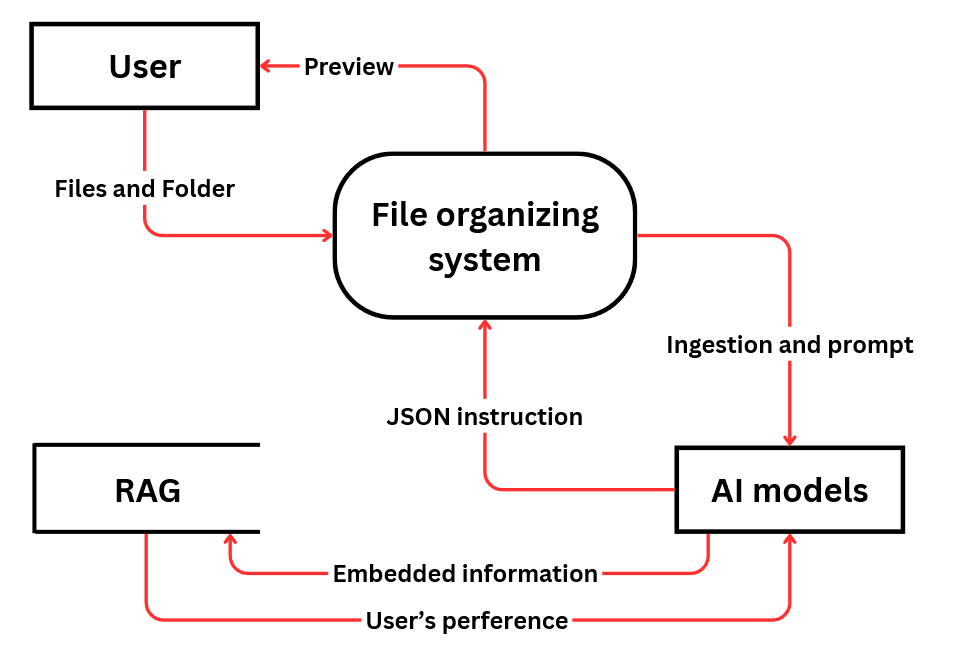
\includegraphics[width=0.9\textwidth]{figures/figure_1.png}
\caption{Dataflow Diagram (level 0)}
\end{figure}
\subsection{Main sequence Diagram}
\begin{figure}[H]\centering
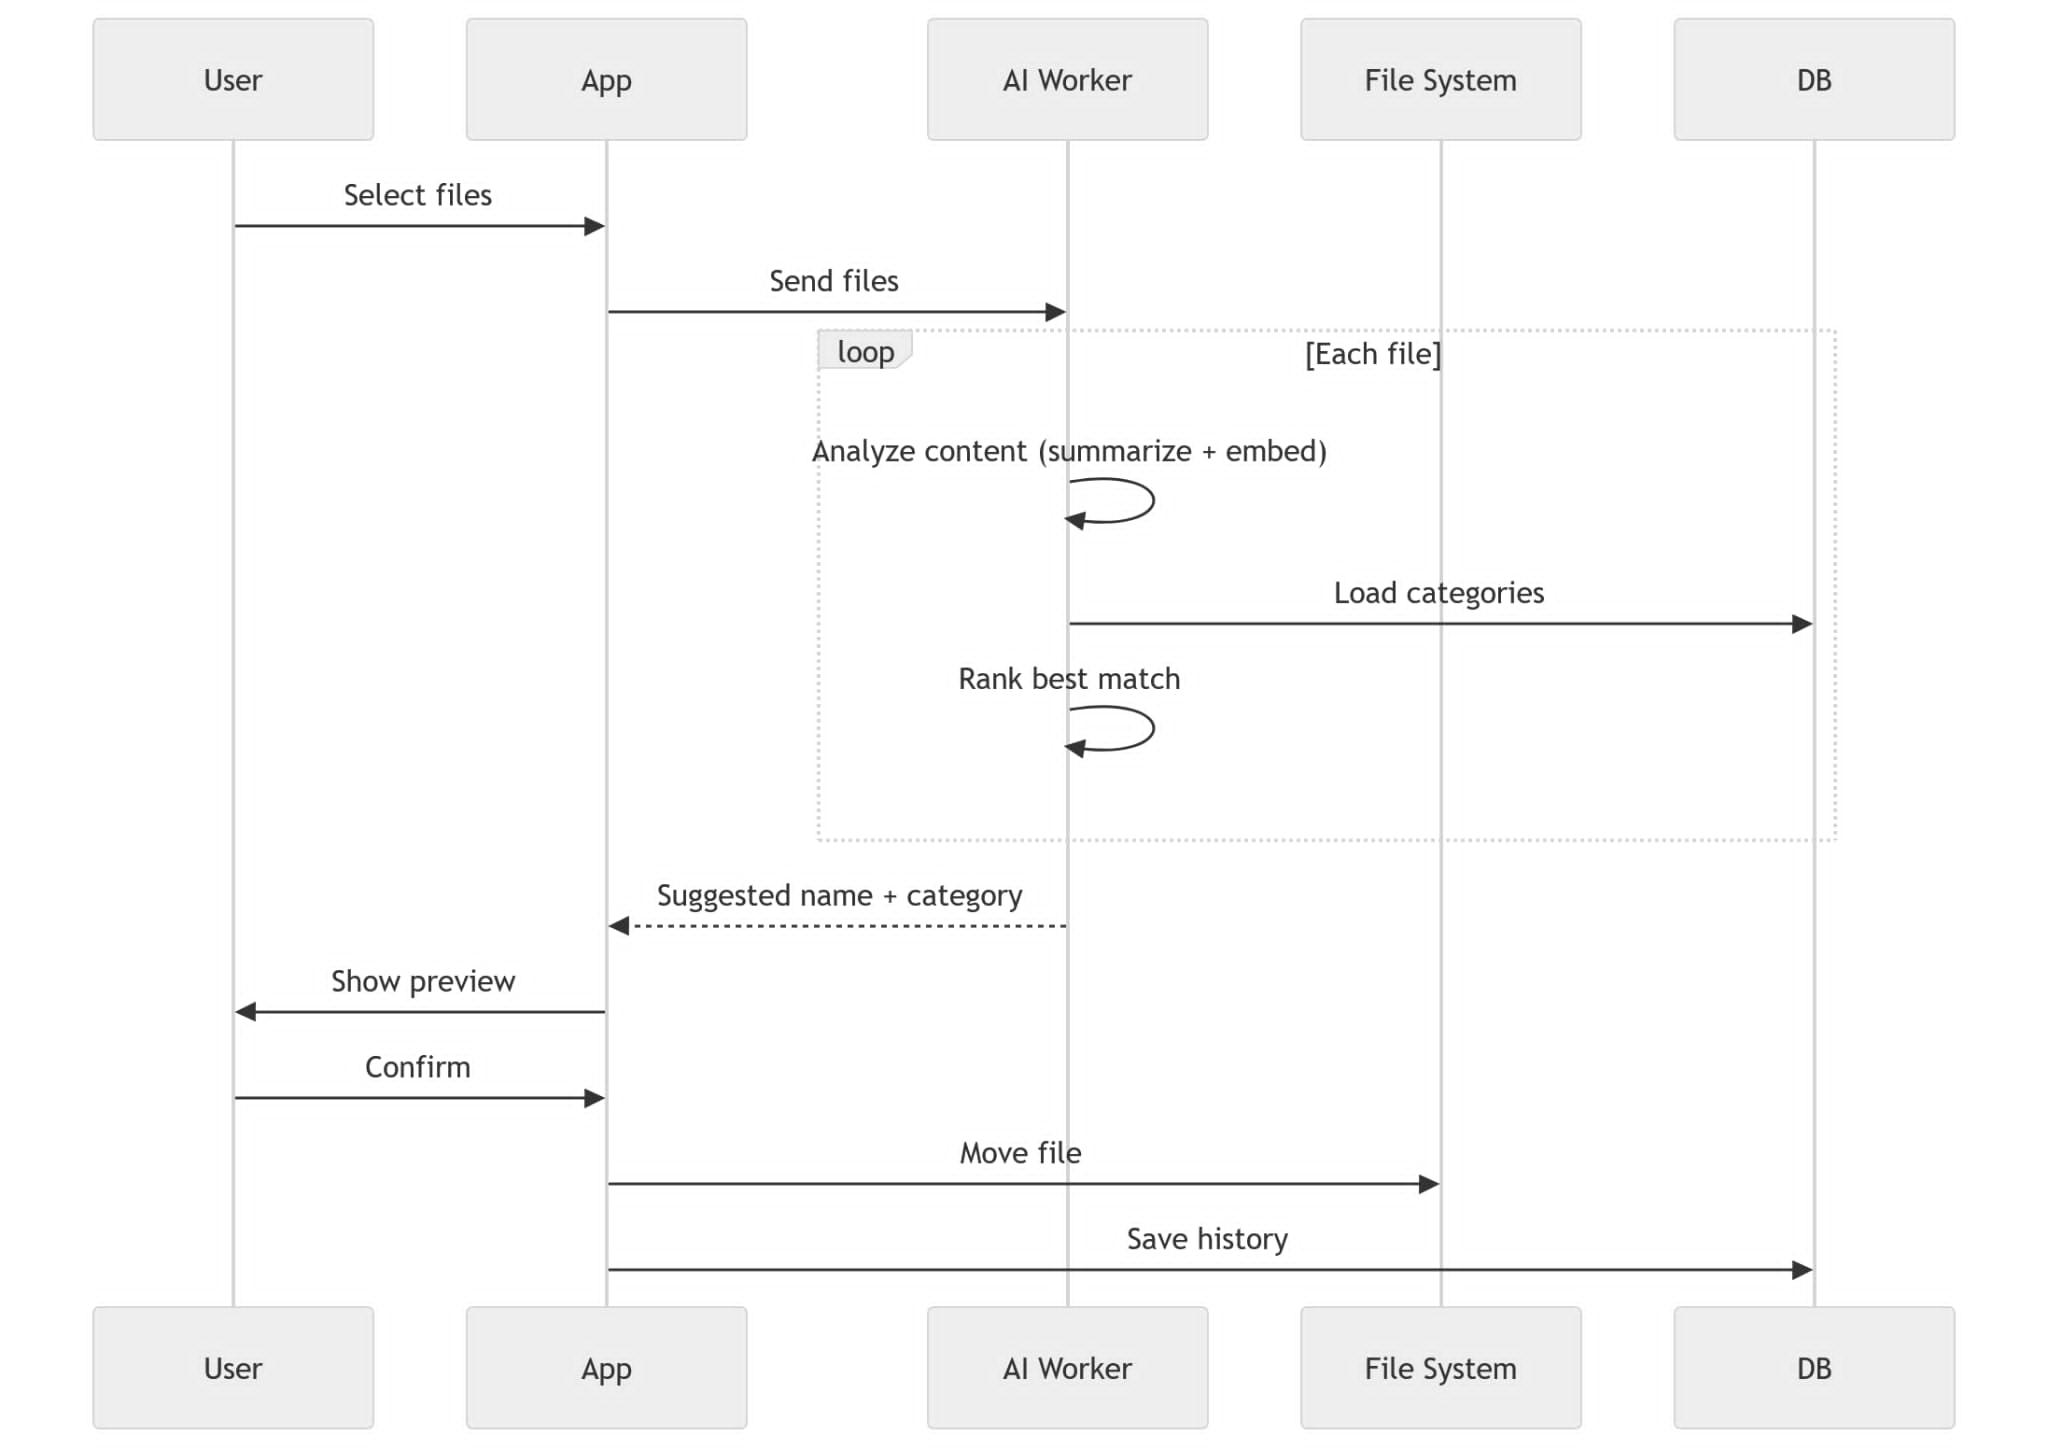
\includegraphics[width=0.9\textwidth]{figures/figure_2.jpg}
\caption{Main Sequence Diagram}
\end{figure}

\subsection{Frontend}
The project is built with Tauri + React. The frontend provides a desktop UI for analyzing dropped files, suggesting categories and names, tracking organization history, and managing settings through a single cohesive interface.

\subsection*{Core development}
\begin{itemize}
\item File Analysis and Intake: Drag-and-drop and file picker mechanisms for capturing files into the organization pipeline
\item Interface for AI models: LLM Models configuration set up
\item Historical Tracking: Comprehensive logging and searchable repository of organization activities
\item Settings and Configuration: User-accessible controls for category management, folder configuration, and automation policies
\item Authentication Integration: Google Calendar API access
\item Background Automation: Real-time monitoring and queued file processing with concurrency control
\end{itemize}
\begin{longtable}{|p{0.22\textwidth}|p{0.20\textwidth}|p{0.48\textwidth}|}
\caption{Tools and Technology implementation in frontend}\\
\hline
\textbf{Component} & \textbf{Technology} & \textbf{Rationale} \\
\hline
UI Framework & React & Modern concurrent rendering with automatic batching \\
\hline
Language & TypeScript & Compile-time type safety and IDE support \\
\hline
Build Tool & Vite & Rapid build times and optimized production bundles \\
\hline
Routing & React Router & Client-side navigation with protected route patterns \\
\hline
State Management & Zustand & Minimalist API with built-in persistence middleware \\
\hline
Component Library & shadcn/ui & Accessible, customizable Radix UI components \\
\hline
Styling & Tailwind CSS & Utility-first CSS with CSS variable theme support \\
\hline
Icons & Lucide React & Lightweight SVG icon library \\
\hline
Desktop Runtime & Tauri & Native desktop integration with Rust backend \\
\hline
Date Handling & date-fns & Functional, modular date manipulation library \\
\hline
Data Visualization & recharts & React-based charting library for metrics display \\
\hline
Notifications & Sonner & Toast notification system for user feedback \\
\hline
Package Manager & Bun & Fast JavaScript runtime and package manager \\
\hline
\end{longtable}

\textbf{Architecture Layer}

The frontend architecture will follow a strict layered structure, where each component is responsible for exactly one concern. The processing pipeline is organized as follows:
\medskip
\vspace{0.5em}

UI → IPC (invoke) → IPC Handler → Command → Service → Infrastructure → Repository
\medskip
\vspace{0.5em}

This design is grounded in the Clean Architecture principle introduced by Robert C. Martin (2012), which states that software should be organized into concentric layers where outer layers depend on inner layers, never the reverse. Each layer in the system maps to a specific responsibility:

\begin{longtable}{|p{0.16\textwidth}|p{0.24\textwidth}|p{0.52\textwidth}|}
\caption{System architecture layers and responsibilities}\\
\hline
\textbf{Layer} & \textbf{Component} & \textbf{Responsibility} \\
\hline
UI & React/TypeScript & Render state and capture user intent \\
\hline
IPC & Tauri invoke() & Serialize and transmit commands across the process boundary \\
\hline
IPC Handler & Tauri command registration & Deserialize input, validate it, and route it to the appropriate command \\
\hline
Command & Rust command functions & Orchestrate one use case end-to-end \\
\hline
Service & Domain service classes & Encapsulate business logic \\
\hline
Infrastructure & File system, watcher, process manager & Execute side effects against the operating system \\
\hline
Repository & JSON / SQLite persistence & Read and write application state \\
\hline
\end{longtable}

In Tauri, the frontend and the backend (Rust) run in separate processes with no shared memory. JavaScript cannot directly access the file system, spawn processes, or interact with the operating system. This is by design, Tauri enforces a strict security boundary between the web context and native capabilities, similar to how web browsers sandbox JavaScript. All cross-boundary calls must pass through the IPC channel (invoke()), which Tauri validates against a declared capability manifest before executing.

This constraint naturally enforces the Separation of Concerns principle (Dijkstra, 1974). The UI layer contains no file-system logic; the repository layer contains no rendering logic. Each layer can be reasoned about, tested, and modified independently. If the storage format for categories changes from JSON to SQLite, only the repository layer changes the command, service, and UI layers are unaffected.

Furthermore, separating the Command layer from the Service layer allows the same business logic (e.g., moving a file and logging the event) to be reused across multiple entry points in a manual user action, an automated watcher trigger, or a future scheduled task without duplicating code.
\vspace{0.2em}

\textbf{Organization Design}

The organization feature is the core workflow of this project. Its design addresses three fundamental challenges:
\begin{enumerate}[label=\arabic*.,leftmargin=0.6in]
\item Files may arrive one at a time or in large batches.
\item AI analysis is slow, non-deterministic, and expensive per call.
\item File moves are irreversible; user confirmation is required before any destructive action.
\end{enumerate}

The full pipeline is divided into four phases: File Discovery, Frontend Queue, AI Analysis, and User Confirmation and Execution.
\vspace{0.2em}

\textbf{Phase 1: File Discovery}
Files enter the organize pipeline through two mutually exclusive triggers:
Trigger A: Manual Selection
The user initiates a native file picker dialog through the UI. Which will cross from IPC boundary into the Rust backend. The Rust command opens the operating system's native dialog using the rfd (Rusty File Dialogs) library and returns the selected paths to the frontend. This approach is used because a native dialog operates with full OS-level permissions and provides a familiar, OS-consistent experience. The JavaScript layer has no direct access to the file system path namespace; Tauri grants it only the specific paths the user explicitly chose.
Trigger B: Automatic Detection via File System Watcher
When the user has configured a watched folder, the Tauri backend registers a file system watcher using the notify crate. When a new file is created or modified in the watched directory, the watcher does not immediately forward the event. Instead, it will apply a two-stage validation:
\begin{itemize}
\item Debounce (500 ms quiet window): File system events fire multiple times during a single write operation. A debounce window collapses all events for the same path into one, preventing duplicate processing.
\item Stability check (polling size and mtime for up to 30 retries): To prevent the system from attempting to analyze a file that is still being downloaded or written (e.g., .crdownload or .part files).
\end{itemize}
Once confirmed, Tauri emits a watched-file-added event to the frontend via the Tauri event system. This design choice keeps the Rust layer decoupled from the AI pipeline and lets the frontend apply the same queue-based flow regardless of how the file was discovered.
\vspace{0.2em}

\textbf{Phase 2: Frontend Queue Architecture}
When files arrive (either from manual selection or from watcher events), the frontend does not immediately dispatch all files to the AI worker in parallel. Instead, it inserts each file path into a sequential analysis queue managed in the Zustand store.
Why is queues necessary:
This decision is justified by the Queue-Based Load Leveling pattern (Microsoft Azure Architecture Patterns, 2023), which states that a queue should be placed between a producer (the UI) and a slow consumer (the AI process) to prevent the consumer from being overwhelmed during load spikes. Specifically:
\begin{enumerate}[label=\arabic*.,leftmargin=0.6in]
\item The AI pipeline is not instantaneous. Each file requires LLM inference for summarization, embedding computation, and cosine similarity scoring against all categories. Processing multiple files in parallel would cause resource contention on the llama-server, increasing total latency per file rather than reducing it.
\item Ordered processing is predictable. A first-in-first-out (FIFO) queue ensures files are processed in the order they were discovered, which matches user expectations when dropping a batch of files.
\item Progress visibility. Because files are in a known queue, the UI can render a progress indicator ("3 of 7 files analyzed") accurately. Without a queue, concurrent fire-and-forget dispatches make it impossible to know the current processing state.
\end{enumerate}

\textbf{Phase 3: AI Analysis}
For each file dequeued, the frontend dispatches an HTTP POST request to backend service, which is a separate Python process (FastAPI) that runs alongside the Tauri app as a sidecar. Separating the AI pipeline into its own process rather than embedding it in Rust or JavaScript is a deliberate architectural choice:
\begin{itemize}
\item Language ecosystem: Python has matured, well-maintained libraries for AI tasks implementing these in Rust would require significant effort with less library support.
\item Process isolation: If the AI worker crashes due to an out-of-memory error or model failure, it does not crash the UI process. The Tauri backend can detect the failure and restart the sidecar independently.
\item Independent scalability: In future versions, the worker could be moved to a remote server without changing the frontend or Tauri code, since they only communicate over HTTP.
\end{itemize}

\textbf{Phase 4: User Confirmation and File Execution}
After the analysis result is returned to the frontend, it presents the user with:
\begin{itemize}
\item A ranked list of category suggestions with confidence scores.
\item Three alternative filename suggestions generated by LLM.
\item The original file path for reference.
\end{itemize}
Why user confirmation is mandatory before any file move:
File moves are destructive and irreversible under normal circumstances (the original path no longer exists) so it requires that users should be able to undo actions or confirm before they are committed.
Upon confirmation, the frontend calls invoke the method to move file. The Tauri Rust backend executes the actual file system operation. Using a Tauri command for the file move, rather than having Python backend process perform it, ensures that the file move is executed by the Rust process that holds the appropriate file system permissions declared in the Tauri capability manifest.
After the move, the frontend writes history sessions to record the original and new paths in the local history store, enabling the undo operation. The undo flow simply reverses the action to move file followed by writing history record event with event type: "undone".



\subsection{Backend}
This project is a privacy-first local file organization system that assists users in categorizing and organizing files based on semantic understanding of file content. The system operates as a desktop application, processing files from absolute paths without uploading or transmitting content outside the local system boundary.

\subsection*{Core development}
\begin{itemize}
\item Scanner Service: Enumerates files from specified directory paths and extracts file metadata: path, size, content hash (SHA-256), extension
\item Classification: Computes cosine similarity between file embeddings and category embeddings
\item RAG Service: A retrieval-augmented generation. Manages the embedding function pipeline, delegating to llama-server. Supporting semantic search
\item Parser: Extracts structured text and tables from PDF, DOCX, XLSX, PPTX, HTML, and Markdown files. Supports two profiles ("fast" and "rich") with configurable for normal OCR or table structure extraction
\item LLM Client: Async HTTP interface to out-of-process llama-server. Essential method for the access of AI. Supporter of the features such as files organization, summary
\item Database: Cache on activity. Participating in workflow for the purpose of reducing workload and remembering the already processed file
\end{itemize}
\begin{longtable}{|p{0.20\textwidth}|p{0.20\textwidth}|p{0.50\textwidth}|}
\caption{Tools and technology implementation in backend}\\
\hline
\textbf{Category} & \textbf{Tool} & \textbf{Purpose} \\
\hline
Framework & FastAPI & Web API framework \\
\hline
Database & SQLAlchemy + SQLModel & Object-relational mapping \\
\hline
Migrations & Alembic & Schema versioning \\
\hline
Parsing & Docling & Multi-format document parsing \\
\hline
RAG & RAG-Anything & Semantic indexing \\
\hline
RAG Backend & LightRAG & Vector storage \\
\hline
LLM & llama.cpp & Local LLM inference as llama-server \\
\hline
Vectors & NumPy & Numerical operations \\
\hline
Logging & logging & Structured logging \\
\hline
Config & dataclass + env & Settings management \\
\hline
\end{longtable}
\subsection*{AI models implementation}
The system must be able to read and support document files, including .pdf, .docx, .pptx, .xlsx and image files. Some file types are easily understood by LLM because they were trained by them, as text base documents, but some like image files (png or .jpeg) cannot be comprehended by normal LLM, and that is the reason why VLM is needed.

With the integration of RAG system and vector database to support semantic search, LLM also need to embedded word from file's content into the vector database which may interfere with its normal process and increasing more time on each session of activity. One of the solutions is to use separate embedding models to handle this job.

This project prioritizes working in local environments, that means special interface is needed. We chose llama.ccp because it requires minimal setup, suitable for offline desktop application.

\subsection*{In summary of this part}
\begin{itemize}
\item All models will be of .gguf format for the use with llama.cpp
\item There will be VLM + mmproj (image encoder support) and embedding model for the best practice
\end{itemize}
\subsection*{Workflow}
The analysis pipeline inside the application applies a cache-first strategy:

\begin{itemize}
\item \textbf{Scan}: The file hash, size, and extension are computed.
\item \textbf{Cache check}: A categories hash is computed from the current set of active categories and the parser profile. If the analysis record already exists in the database for this file with a matching hash, the cached analysis is returned immediately and no LLM call is made.
\item \textbf{Parse}: If the cache misses, the file is parsed using Docling's fast profile to extract text content. The result is a structured summary suitable for LLM input.
\item \textbf{Summarize}: The extracted text is sent to the llama-server chat endpoint with a summarization prompt. For image files, the vision-capable model endpoint is used instead.
\item \textbf{Rename suggestion}: The summary is sent to the LLM with a rename prompt that instructs the model to produce filenames. The output is post-processed with sanitization rules to ensure filesystem compatibility.
\item \textbf{Embedding and classification}: The file summary is embedded using the llama-server embedding endpoint. The resulting vector is compared against the pre-computed embedding of each active category using cosine similarity.
\item \textbf{Persist}: The analysis result is written to the database and a history entry is created.
\end{itemize}

So, the basic workflow should be like this:

[Stage 1] Scan Files

\begin{itemize}
\item Enumerate file paths
\item Compute file hashes and metadata
\item Load existing File records from database
\item Determine which files have changed
\end{itemize}
\noindent\hspace*{0.6in}↓

[Stage 2] Cache Check

\begin{itemize}
\item If unchanged \& categories match → Hit (return cached results)
\item If categories changed but file unchanged → Partial (re-classify only)
\item If file changed or forced → Full pipeline
\end{itemize}
\noindent\hspace*{0.6in}↓

[Stage 3a: Full pipeline] Parse \& Queue Background Ingestion

\begin{itemize}
\item Parsing and extracting
\item Enqueue file into background RAG ingestion
\end{itemize}
\noindent\hspace*{0.6in}↓

[Stage 3b] Generate Summary (if not cached)

\begin{itemize}
\item If image: send to VLM
\item If text: use extracted text + LLM summary
\item If neither: filename fallback
\end{itemize}
\noindent\hspace*{0.6in}↓

[Stage 4] Generate Rename Suggestions (if summary available)

\begin{itemize}
\item LLM generates N candidate filenames based on summary
\item Sanitize and validate suggestions
\end{itemize}
\noindent\hspace*{0.6in}↓

[Stage 5] Classify Files

\begin{itemize}
\item Compute file embedding (filename + summary)
\item Load active categories with embeddings
\item Compute cosine similarity for each category
\item Sort by score descending; retain top-K
\end{itemize}
\noindent\hspace*{0.6in}↓

[Stage 6] Return Results

\begin{itemize}
\item Format response with scores, suggestions, metadata
\item Log history activity
\end{itemize}
\noindent\hspace*{0.6in}↓

[Response] (with scores, suggestions, timings)

\section{Evaluation method}
To conform with objectives of this project which is a service invention project in the form of a desktop application, the evaluation method must include both Performance testing and End-user opinion. To cover both aspects in a structured way, the evaluation strategy of this project is organized into three complementary layers, each answering a different question about the system:

\begin{itemize}
\item \textbf{Automated testing (code-level):} Unit tests written alongside the source code to verify the correctness of individual functions, modules, and persistence layers. The frontend will be tested with the Bun test runner. The backend is tested with cargo test lib. All tests organized in a dedicated \texttt{*/tests/} module. This layer protects against regressions during development and enforces the data contract between the frontend and backend.
\item \textbf{Persona-based benchmark (system-level):} An automated functional benchmark that measures the application's file-classification accuracy on realistic test files grouped by user persona (Student, HR Officer, Designer). This layer answers whether the system behaves correctly on real-world inputs.
\item \textbf{Expert evaluation form (user-level):} A questionnaire-based evaluation completed by experts in computer engineering or software development. The questions are derived from the project objectives, and an odd number of experts participate so that a consensus on the application's success can be obtained.
\end{itemize}
Among the three layers, the Expert Evaluation form is treated as the primary qualitative method for the overall performance analysis and conclusion of this project, while the automated tests and the persona-based benchmark provide the supporting quantitative evidence.

\chapter{Results and Analysis}
\section{Finished Product}
The project ``AI-powered file organizer application'', named KLIN, was conducted according to the following steps:

\begin{itemize}
\item Studying project-related information
\item Developing a demo application and testing the LLM model
\item Creating an expert evaluation form for application performance
\item Collecting data for development and improvement
\item Analyzing data and summarizing the project results
\end{itemize}

The remainder of this section presents the finished application through screenshots of the actual product, grouped by feature area:

\subsection*{First-Time Setup}
When KLIN is launched for the first time, it guides the user through a short setup process. The user is welcomed by the setup screen, the required local AI models are downloaded, and a four-step wizard collects the base path, categories, and watched folders. All AI models run entirely on the user's device, so files and notes never leave the local machine.

\begin{figure}[H]\centering

\includegraphics[width=0.9\textwidth]{figures/feature/feat_setup_welcome.png}
\caption{The first-time setup welcome screen}
\end{figure}

\begin{figure}[H]\centering
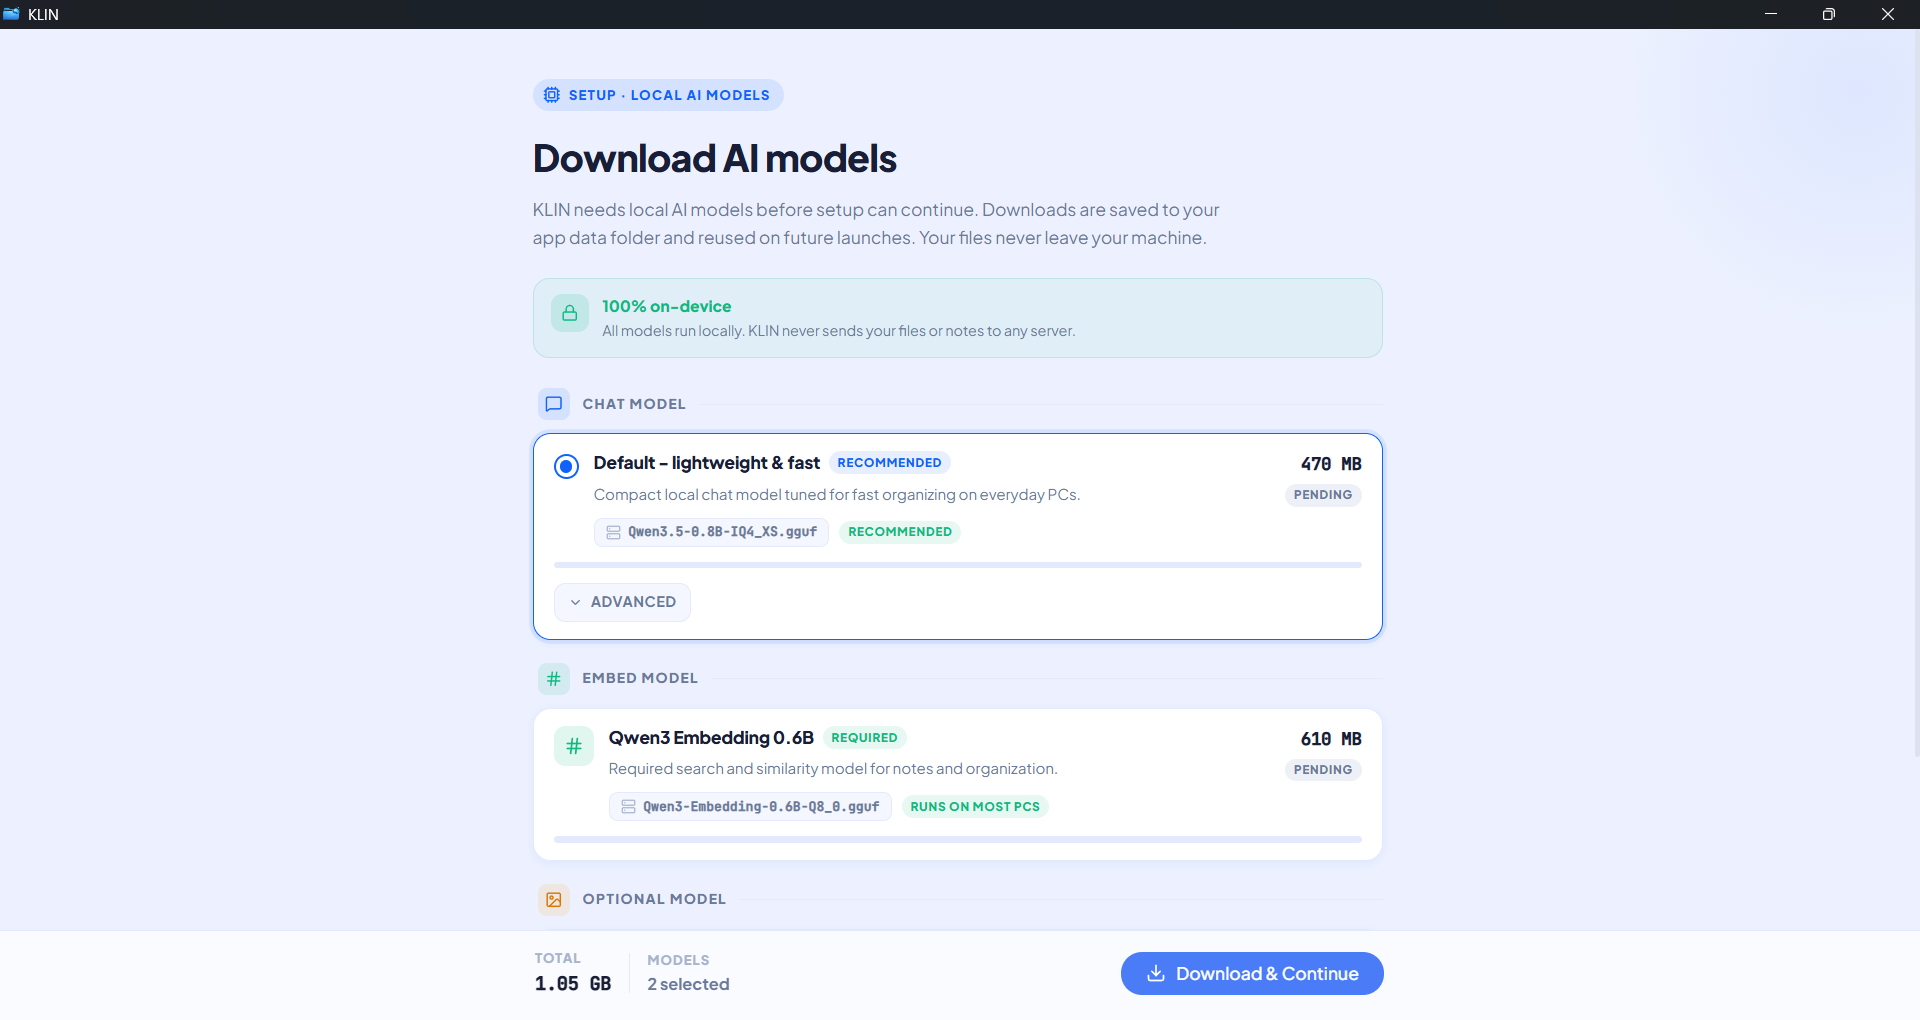
\includegraphics[width=0.9\textwidth]{figures/feature/feat_setup_models.png}
\caption{Downloading the local AI models during setup; all models run on-device}
\end{figure}

\begin{figure}[H]\centering
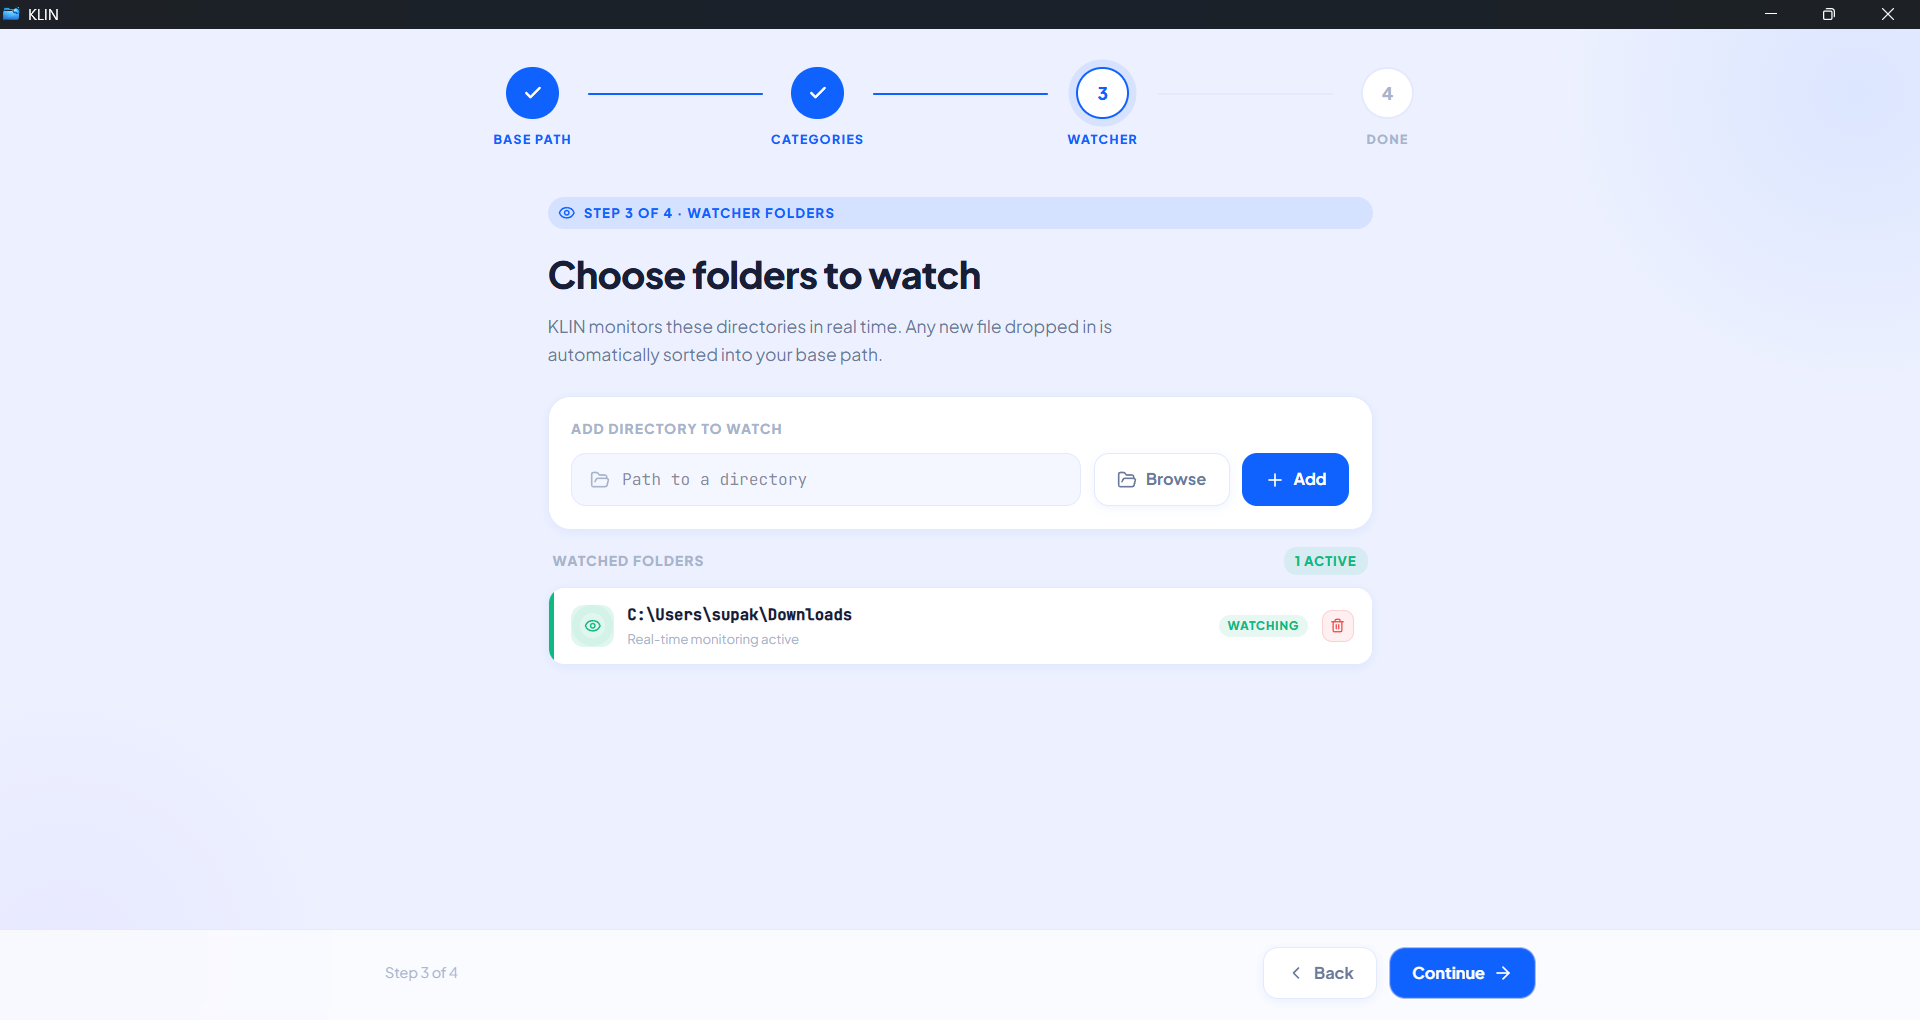
\includegraphics[width=0.9\textwidth]{figures/feature/feat_setup_wizard.png}
\caption{The guided four-step setup wizard (base path, categories, watched folders, and confirmation)}
\end{figure}

\subsection*{Dashboard}
The Dashboard is the main screen of the application. It summarizes the organized categories and their file counts, provides the AI Organizer drop zone for adding new files, and displays a live activity feed of recent file movements.

\begin{figure}[H]\centering
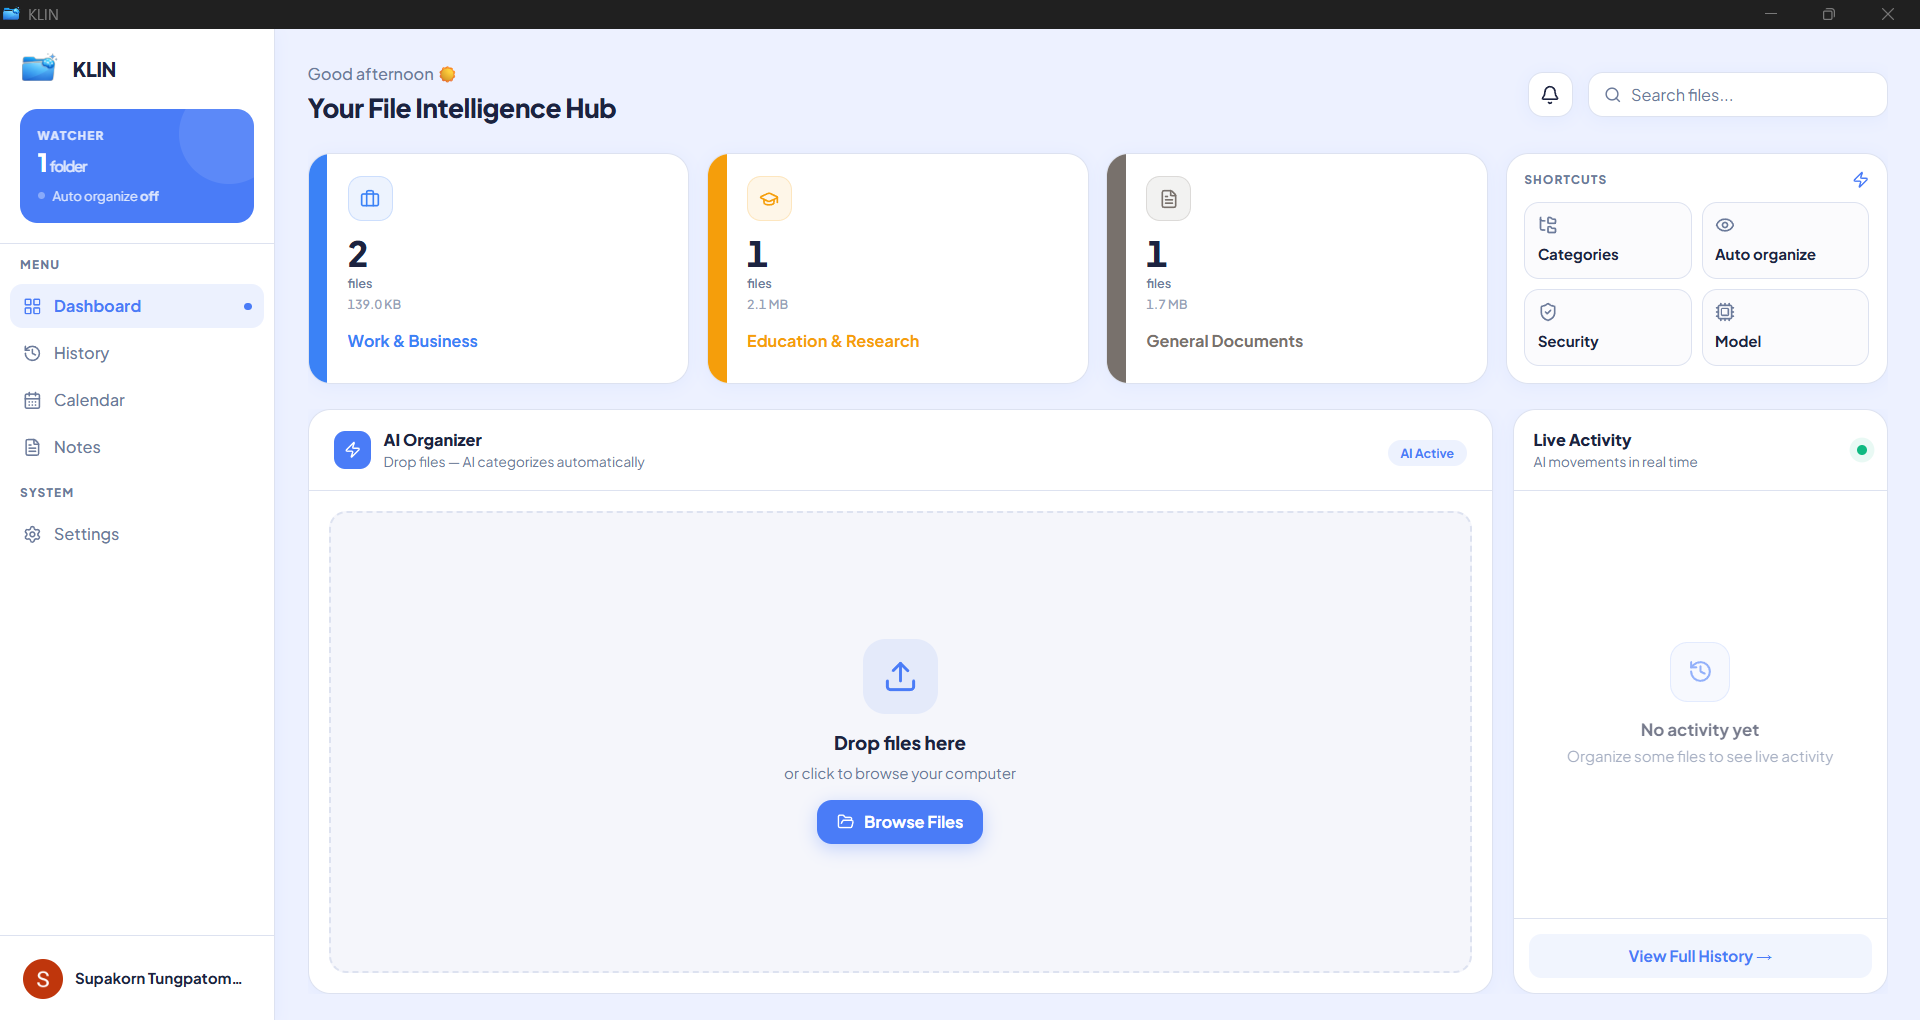
\includegraphics[width=0.9\textwidth]{figures/feature/feat_dashboard.png}
\caption{The Dashboard (File Intelligence Hub) of the application}
\end{figure}

\subsection*{AI File Organizer}
The AI File Organizer is the core feature of the application. After files are added, the system analyzes each file's content and presents the top five category suggestions together with the proposed destination folder. The user reviews these suggestions in a preview before approving the move.

\begin{figure}[H]\centering
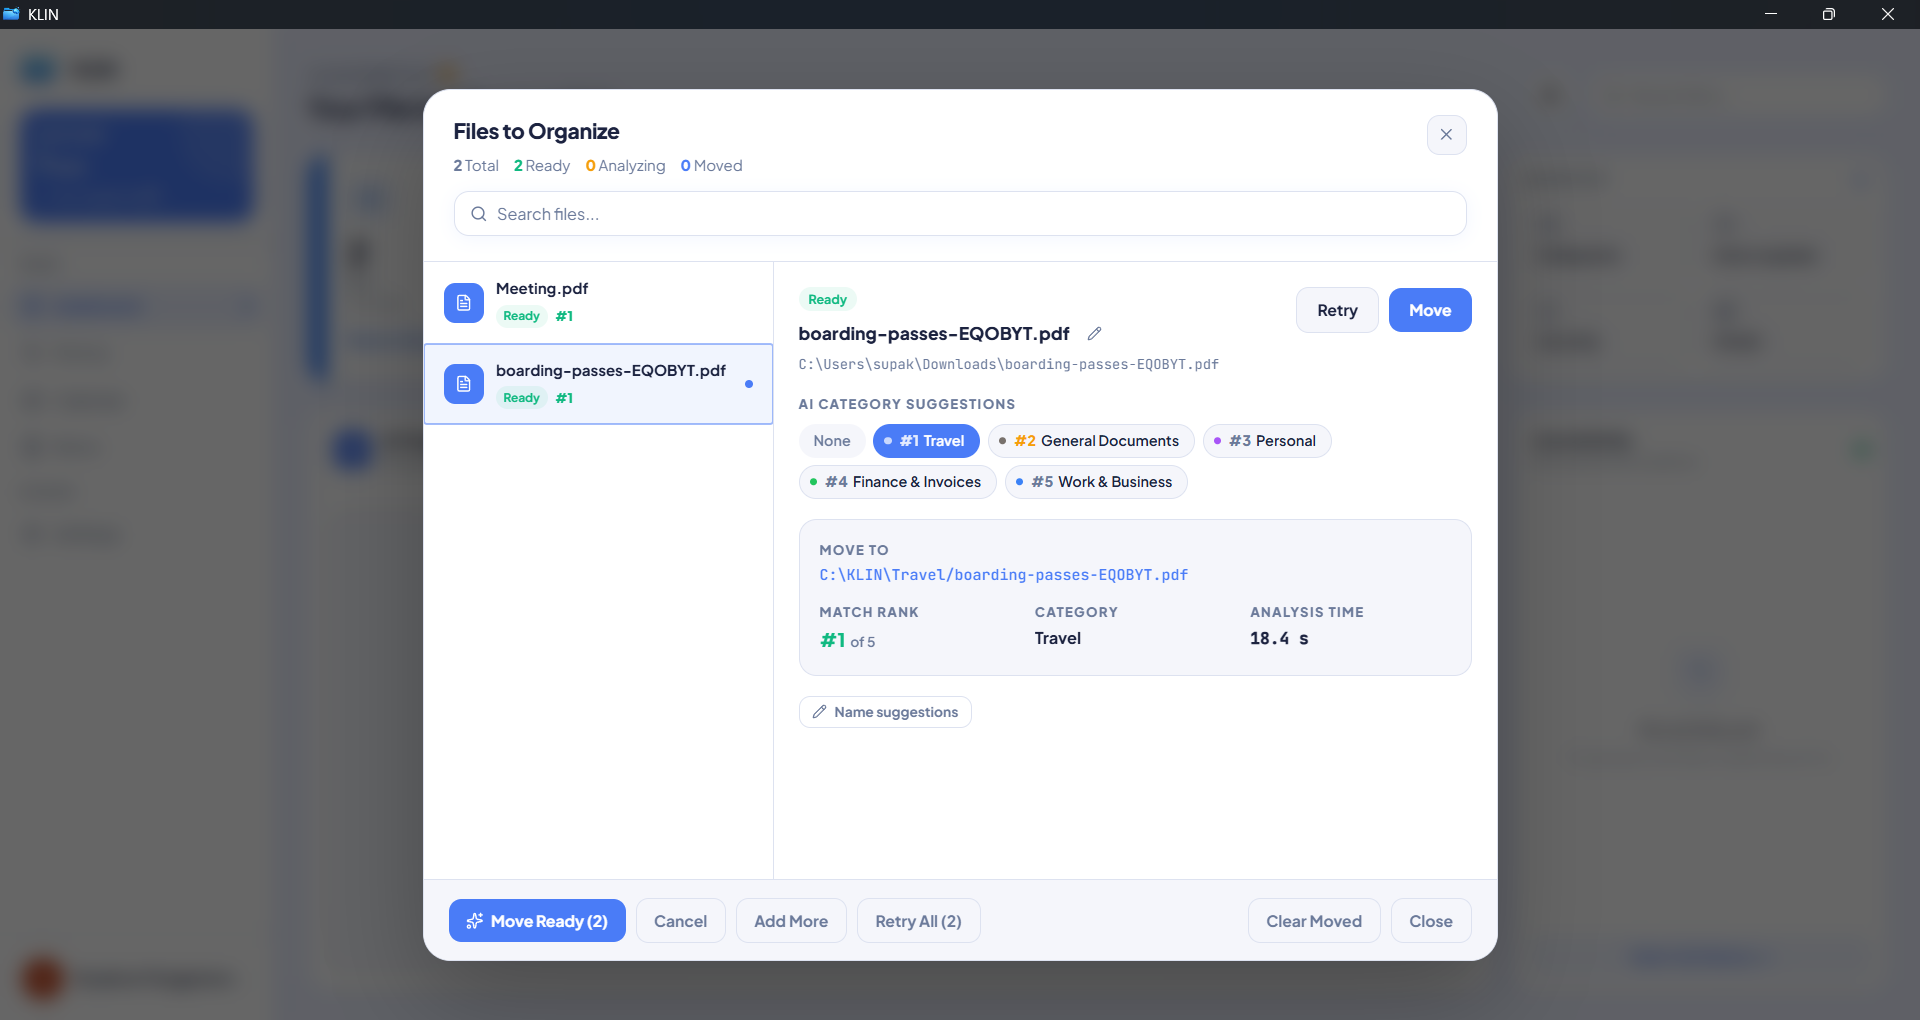
\includegraphics[width=0.9\textwidth]{figures/feature/feat_organize_suggest.png}
\caption{The AI Organizer showing the top-five category suggestions and the proposed destination for a file}
\end{figure}

\begin{figure}[H]\centering
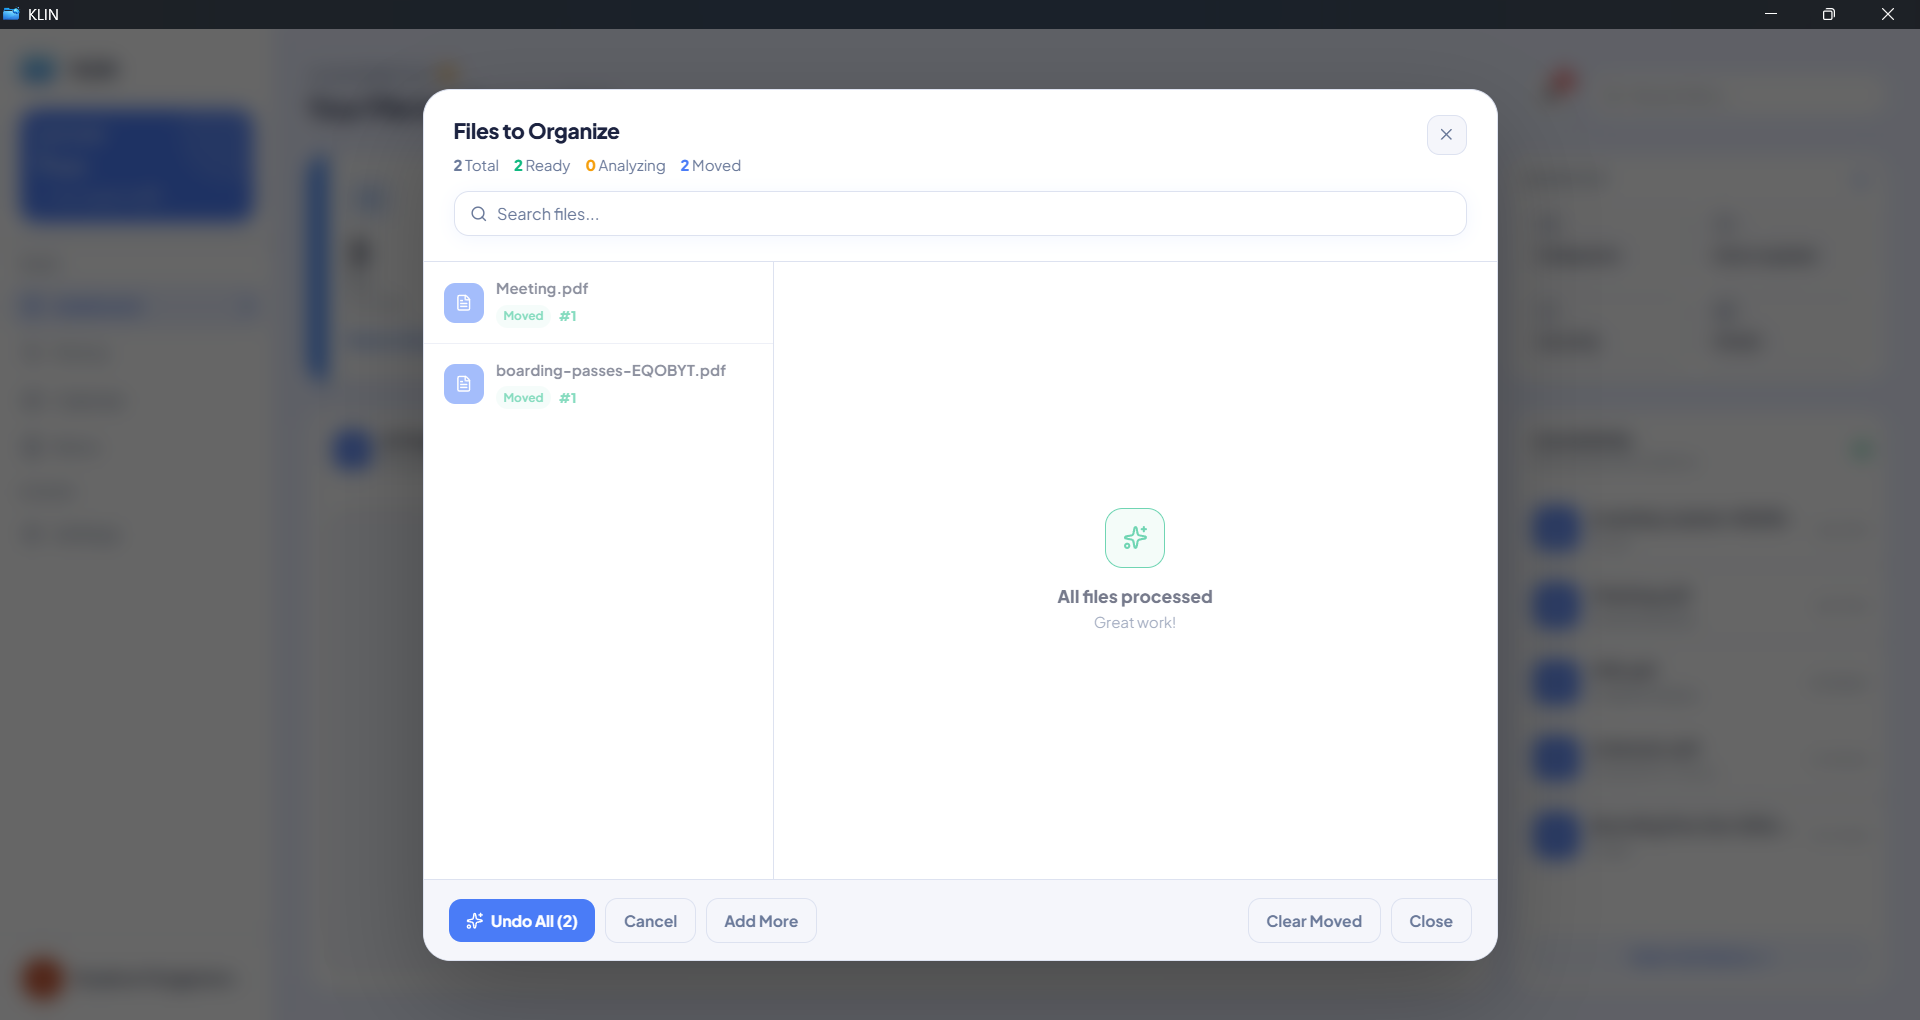
\includegraphics[width=0.9\textwidth]{figures/feature/feat_organize_done.png}
\caption{The AI Organizer after all files have been processed and moved}
\end{figure}

\subsection*{Activity History}
Every file operation performed by the application is recorded in the Activity History page. Each entry can be reverted individually, and the page also supports undoing or redoing all recorded operations.

\begin{figure}[H]\centering
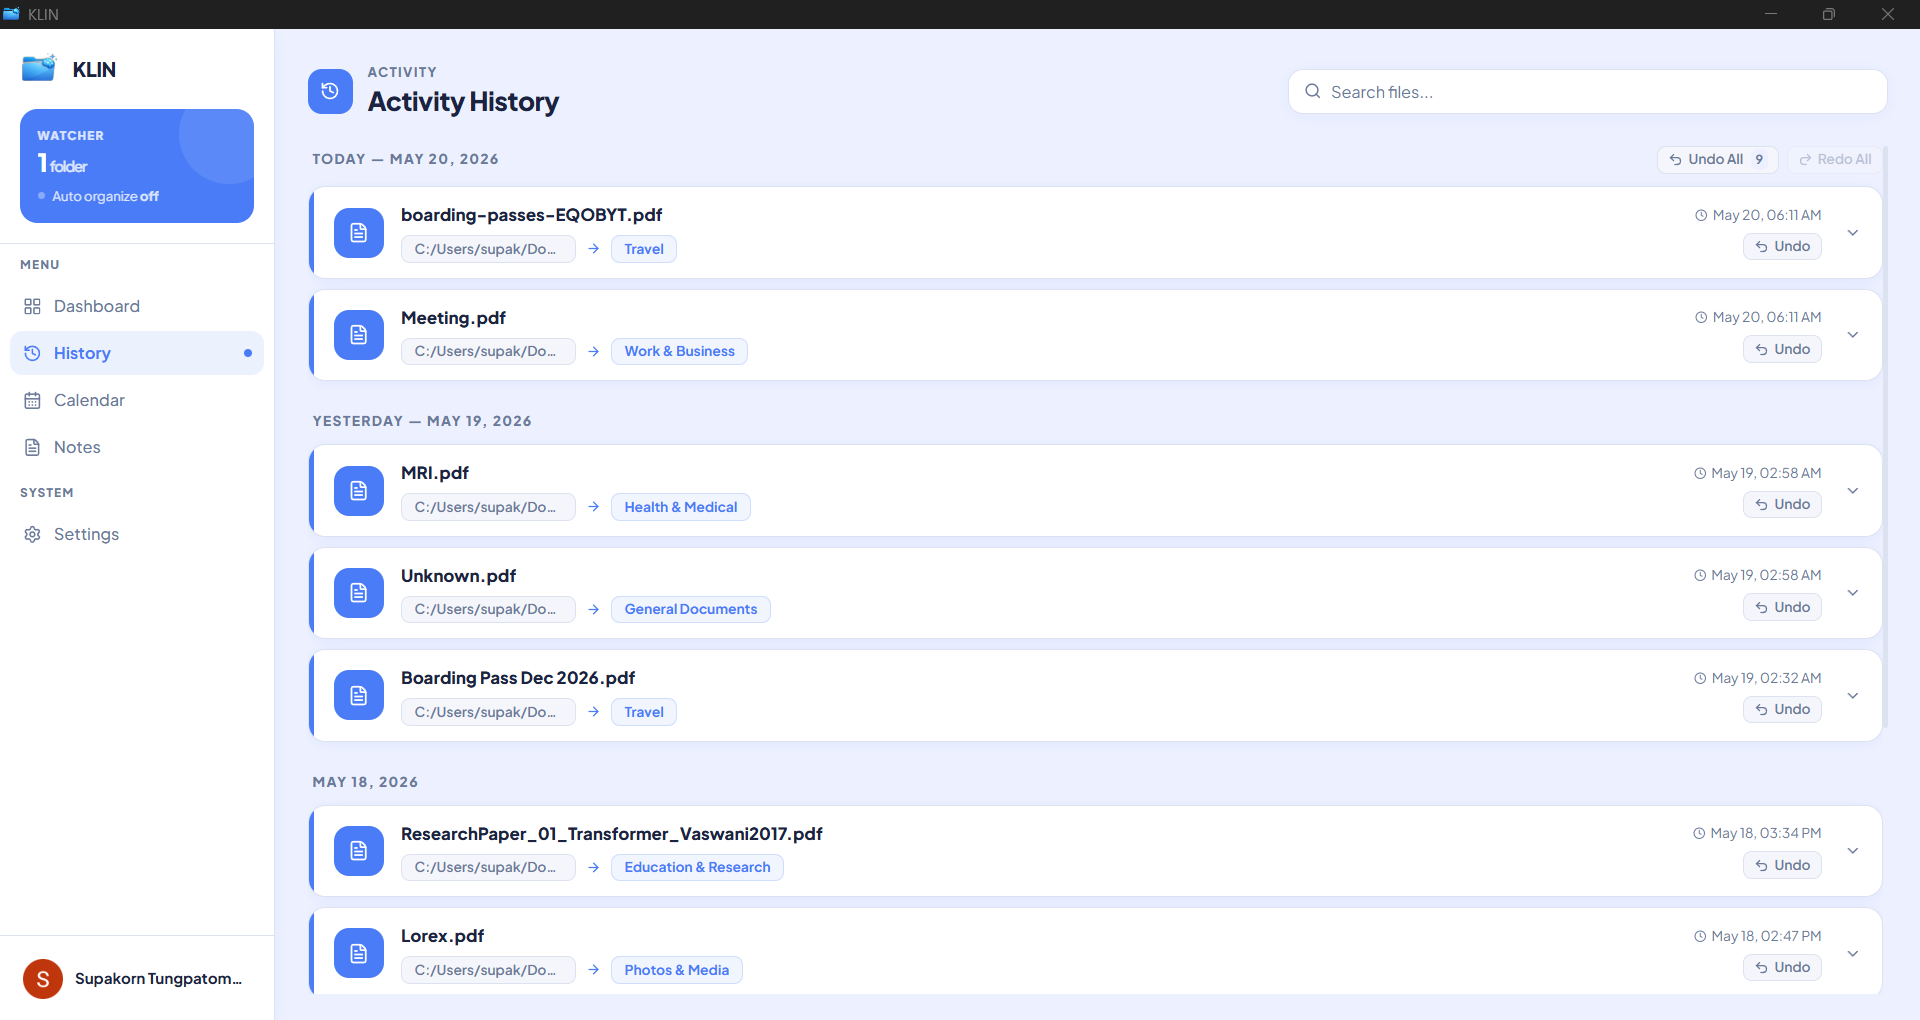
\includegraphics[width=0.9\textwidth]{figures/feature/feat_history.png}
\caption{The Activity History page, listing every file operation with per-item Undo}
\end{figure}

\subsection*{Calendar Integration}
The application can detect calendar events contained in documents, such as meeting or interview dates, and add them to the user's Google Calendar. The Calendar page displays these events and stays synchronized with Google Calendar.

\begin{figure}[H]\centering
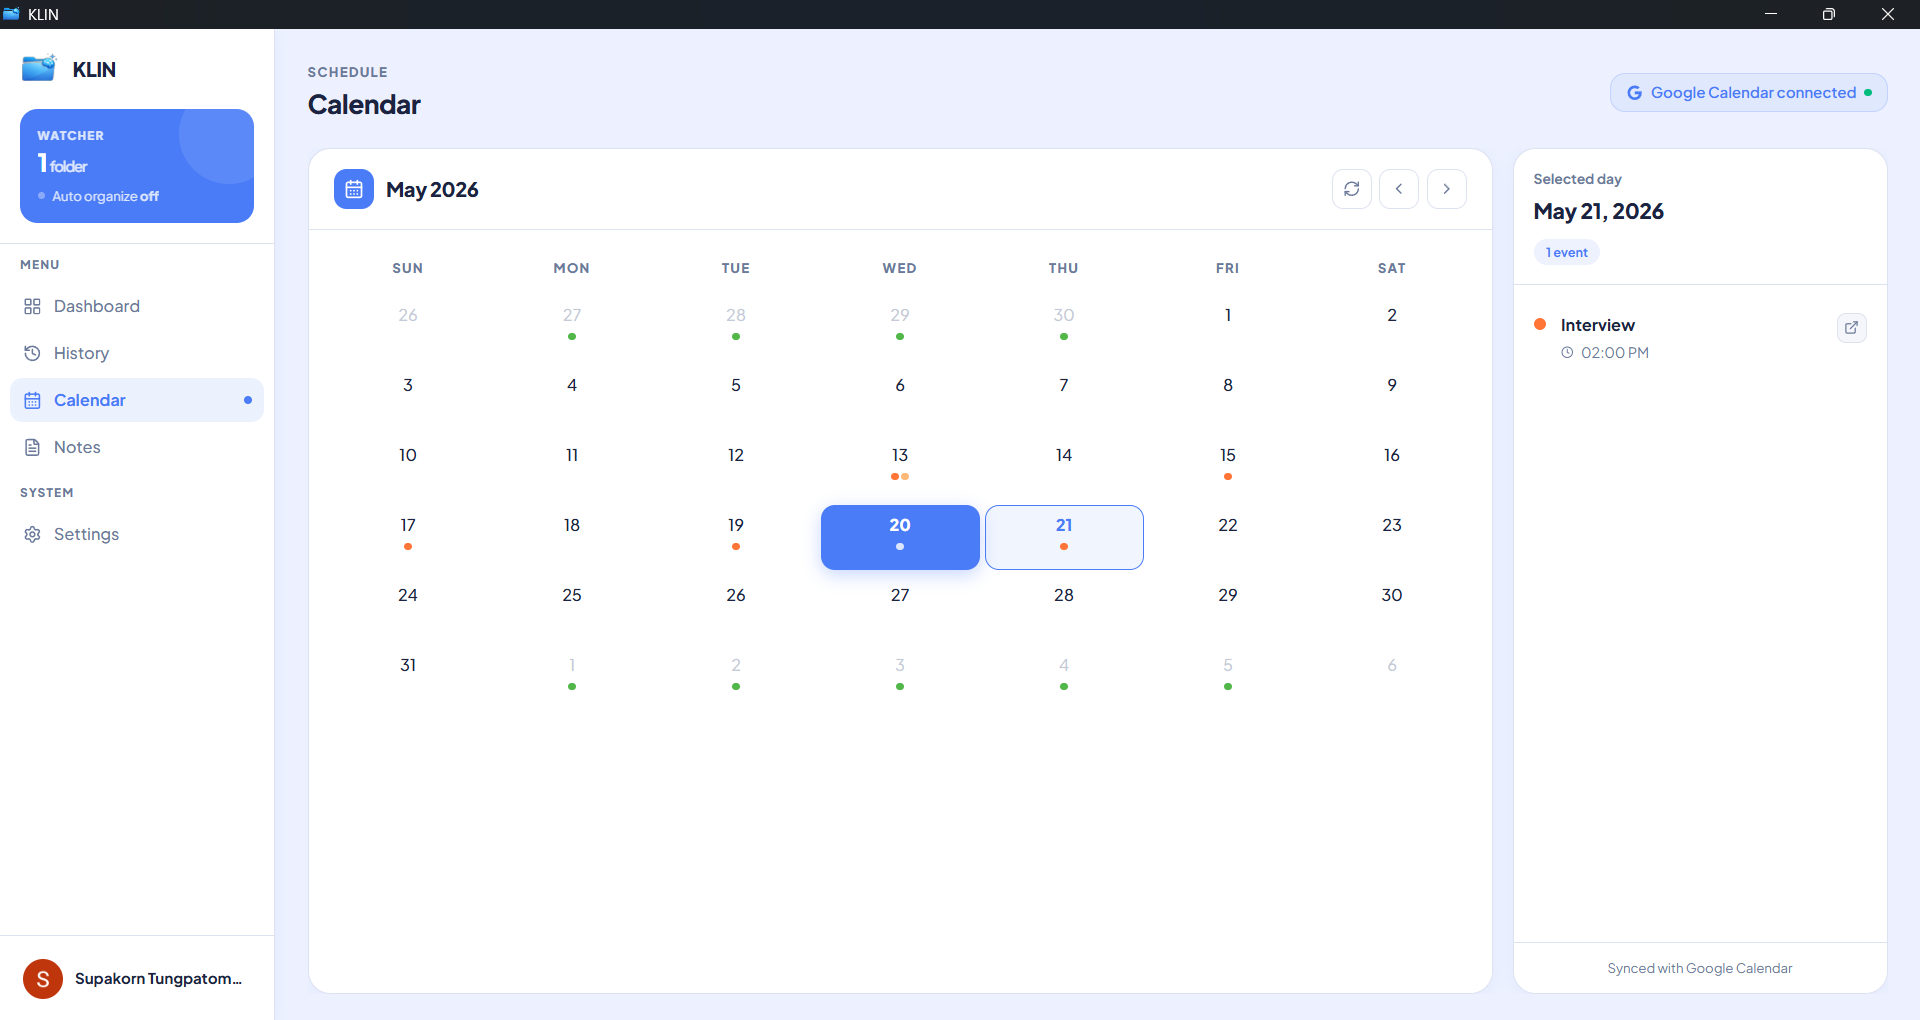
\includegraphics[width=0.9\textwidth]{figures/feature/feat_calendar.png}
\caption{The Calendar page, synchronized with Google Calendar}
\end{figure}

\begin{figure}[H]\centering
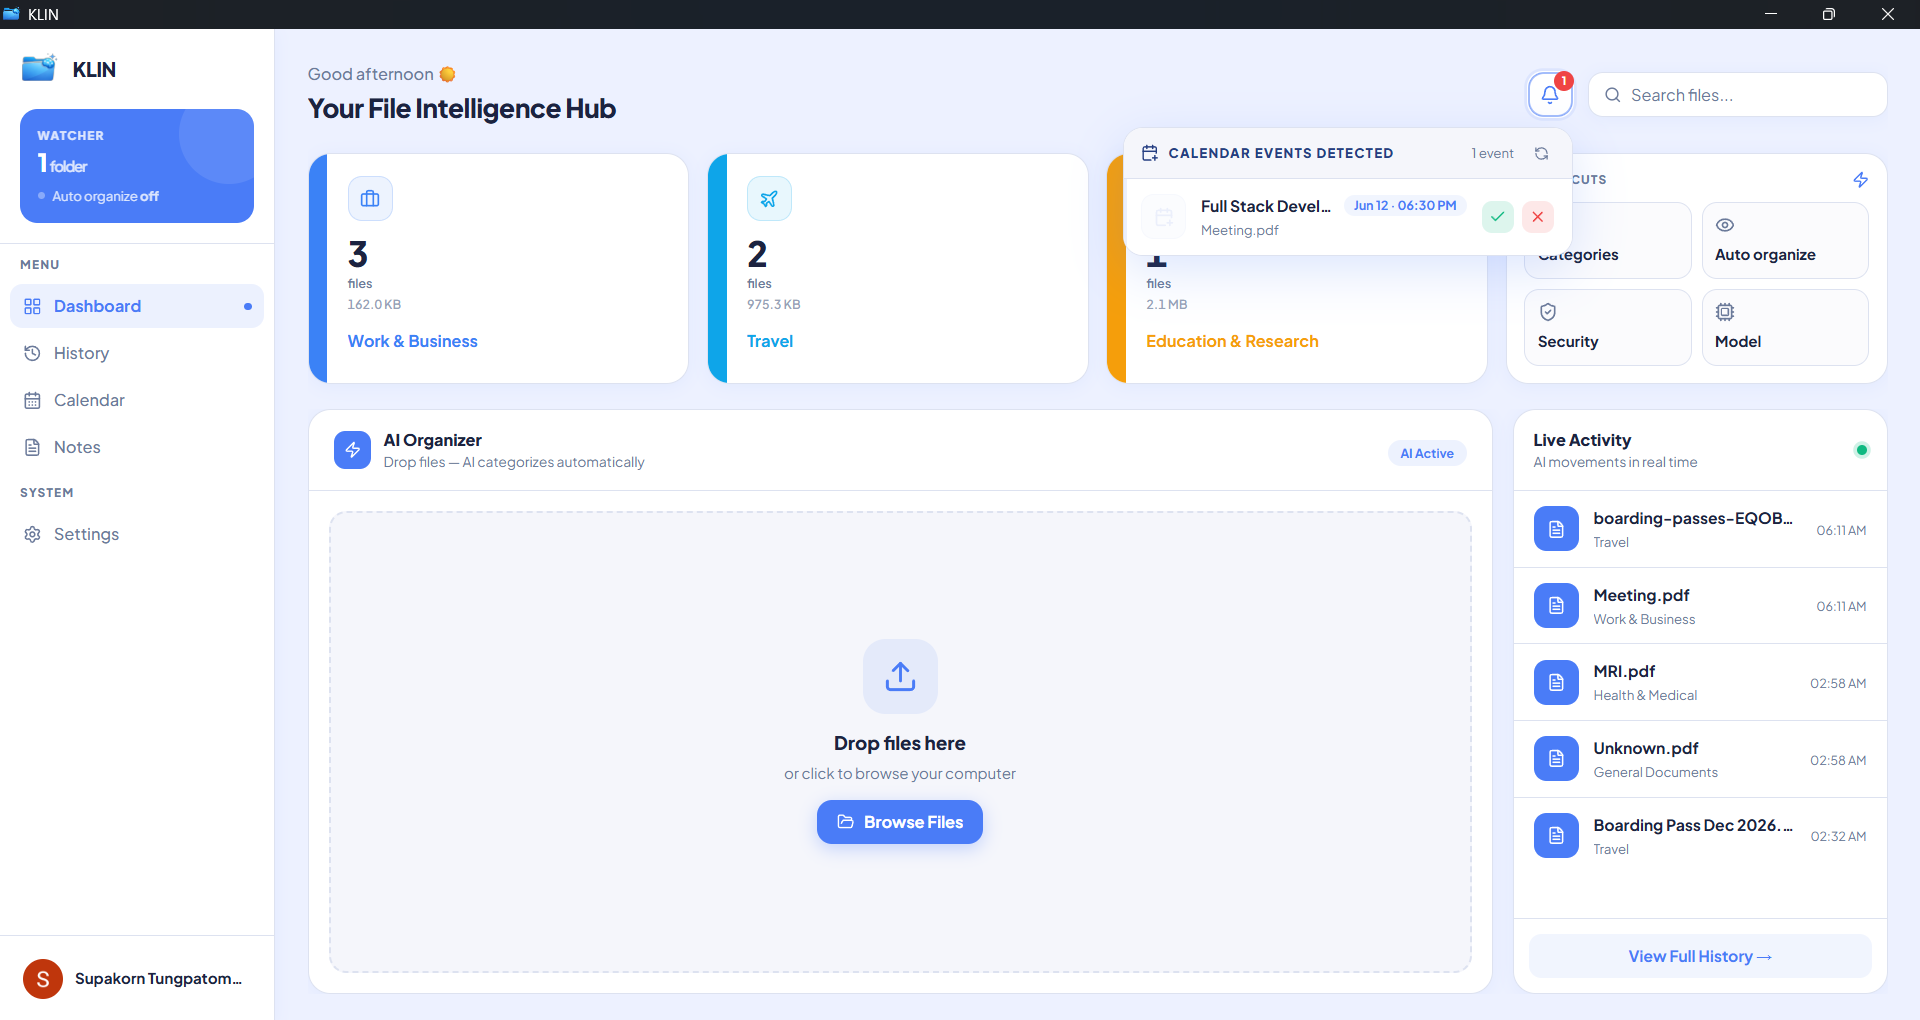
\includegraphics[width=0.9\textwidth]{figures/feature/feat_calendar_detect.png}
\caption{Automatic detection of a calendar event extracted from a document}
\end{figure}

\subsection*{Notes and AI Summaries}
The Notes page lets users keep notes alongside their files. Using the AI Summarize function, the application can read a document and generate a concise summary note, allowing the user to understand a file's content without opening it.

\begin{figure}[H]\centering
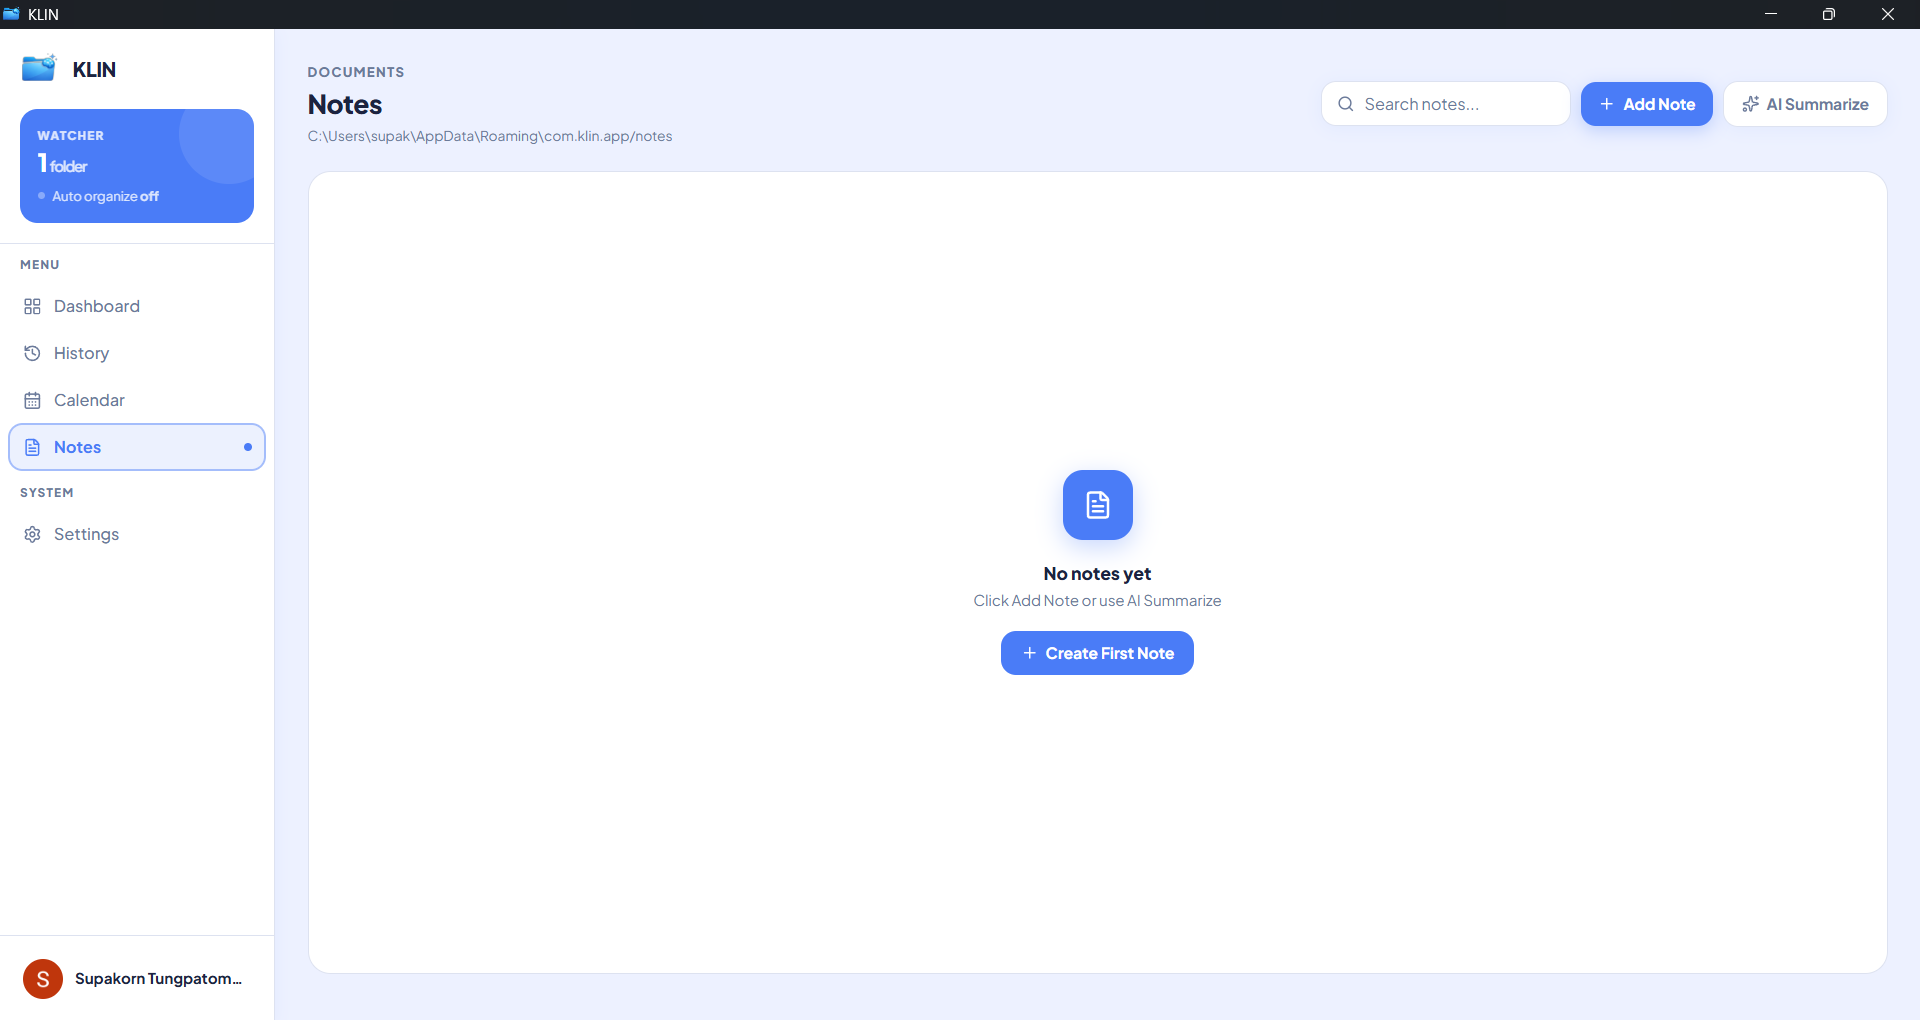
\includegraphics[width=0.9\textwidth]{figures/feature/feat_notes.png}
\caption{The Notes page of the application}
\end{figure}

\begin{figure}[H]\centering
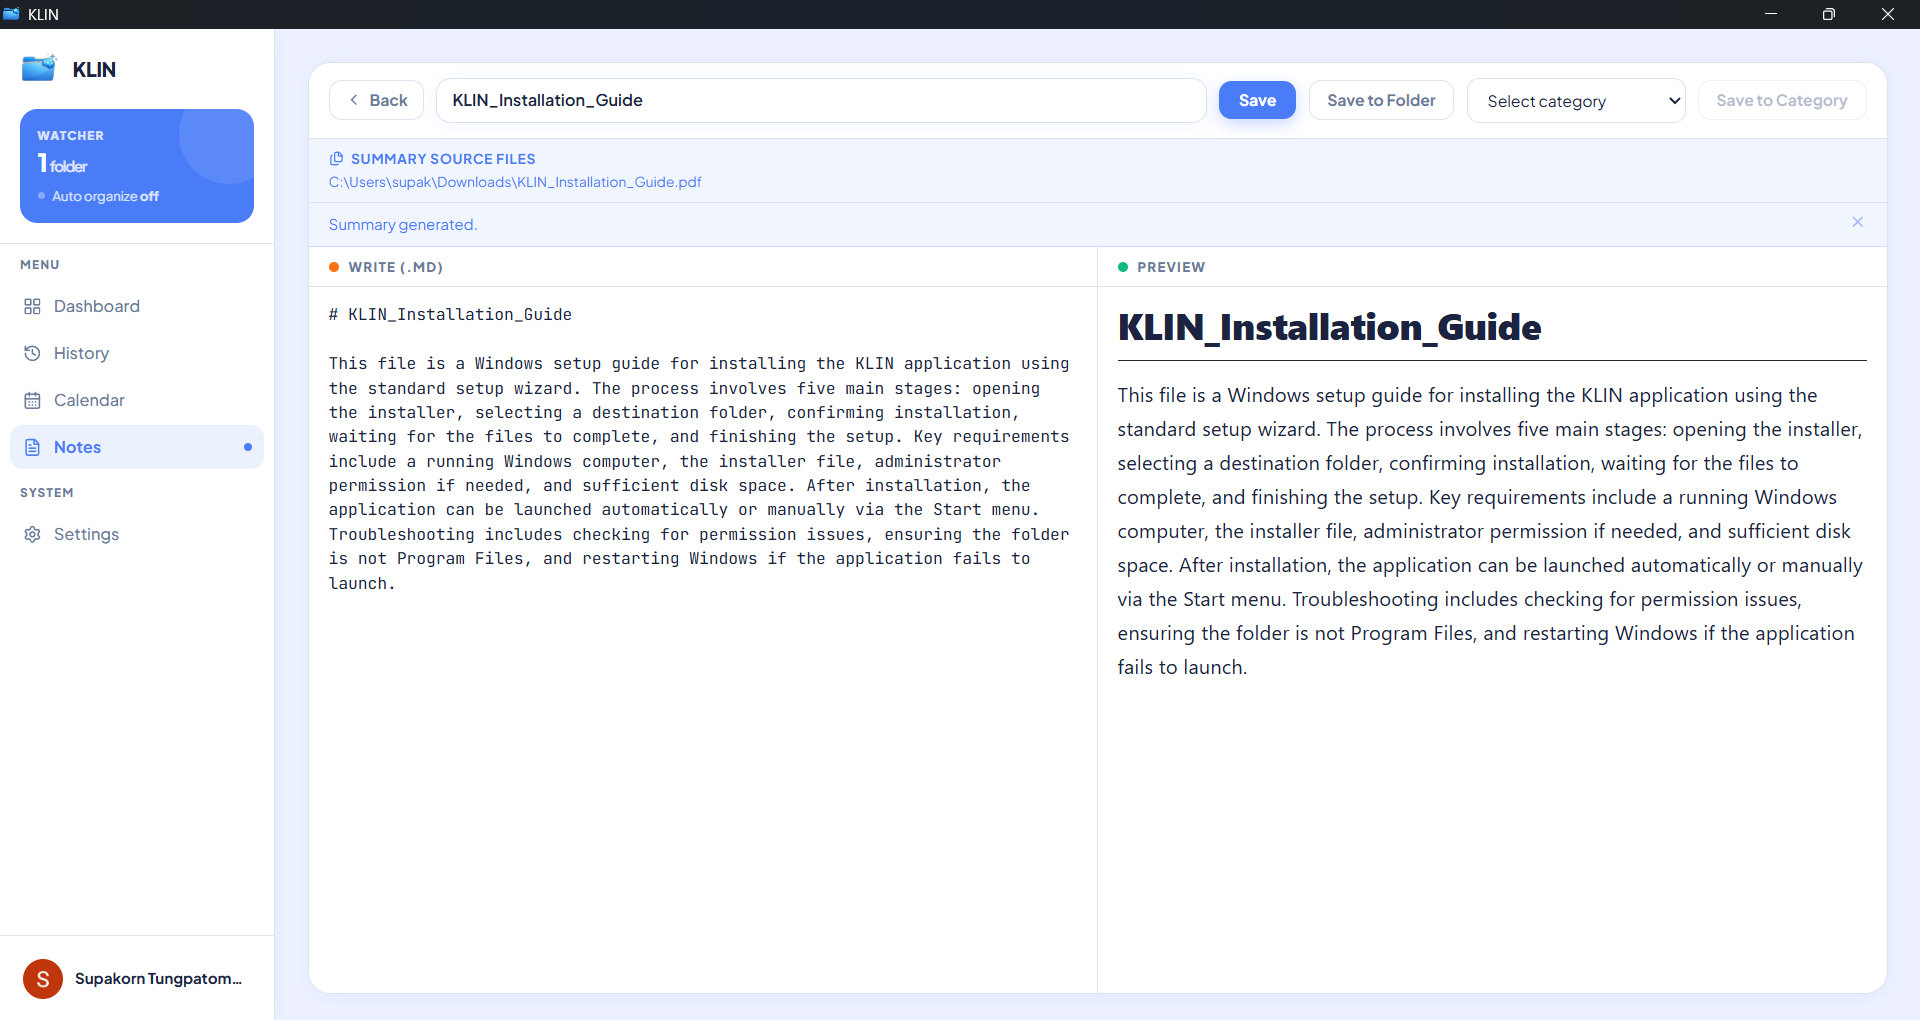
\includegraphics[width=0.8\textwidth]{figures/feature/feat_note_summary.png}
\caption{An AI-generated summary note created from a document}
\end{figure}

\subsection*{Application Settings}
The Settings page is divided into five sections. The Account section manages the connected Google account; Configuration sets the default output folder, watched folders, and AI categories, and can also import an existing folder structure as categories in a single batch operation; Automation controls the Auto Organize background watcher and manual scanning; Model manages the local AI models; and Security provides a vault for locking files and folders so that they are never sent to the AI.

\begin{figure}[H]\centering
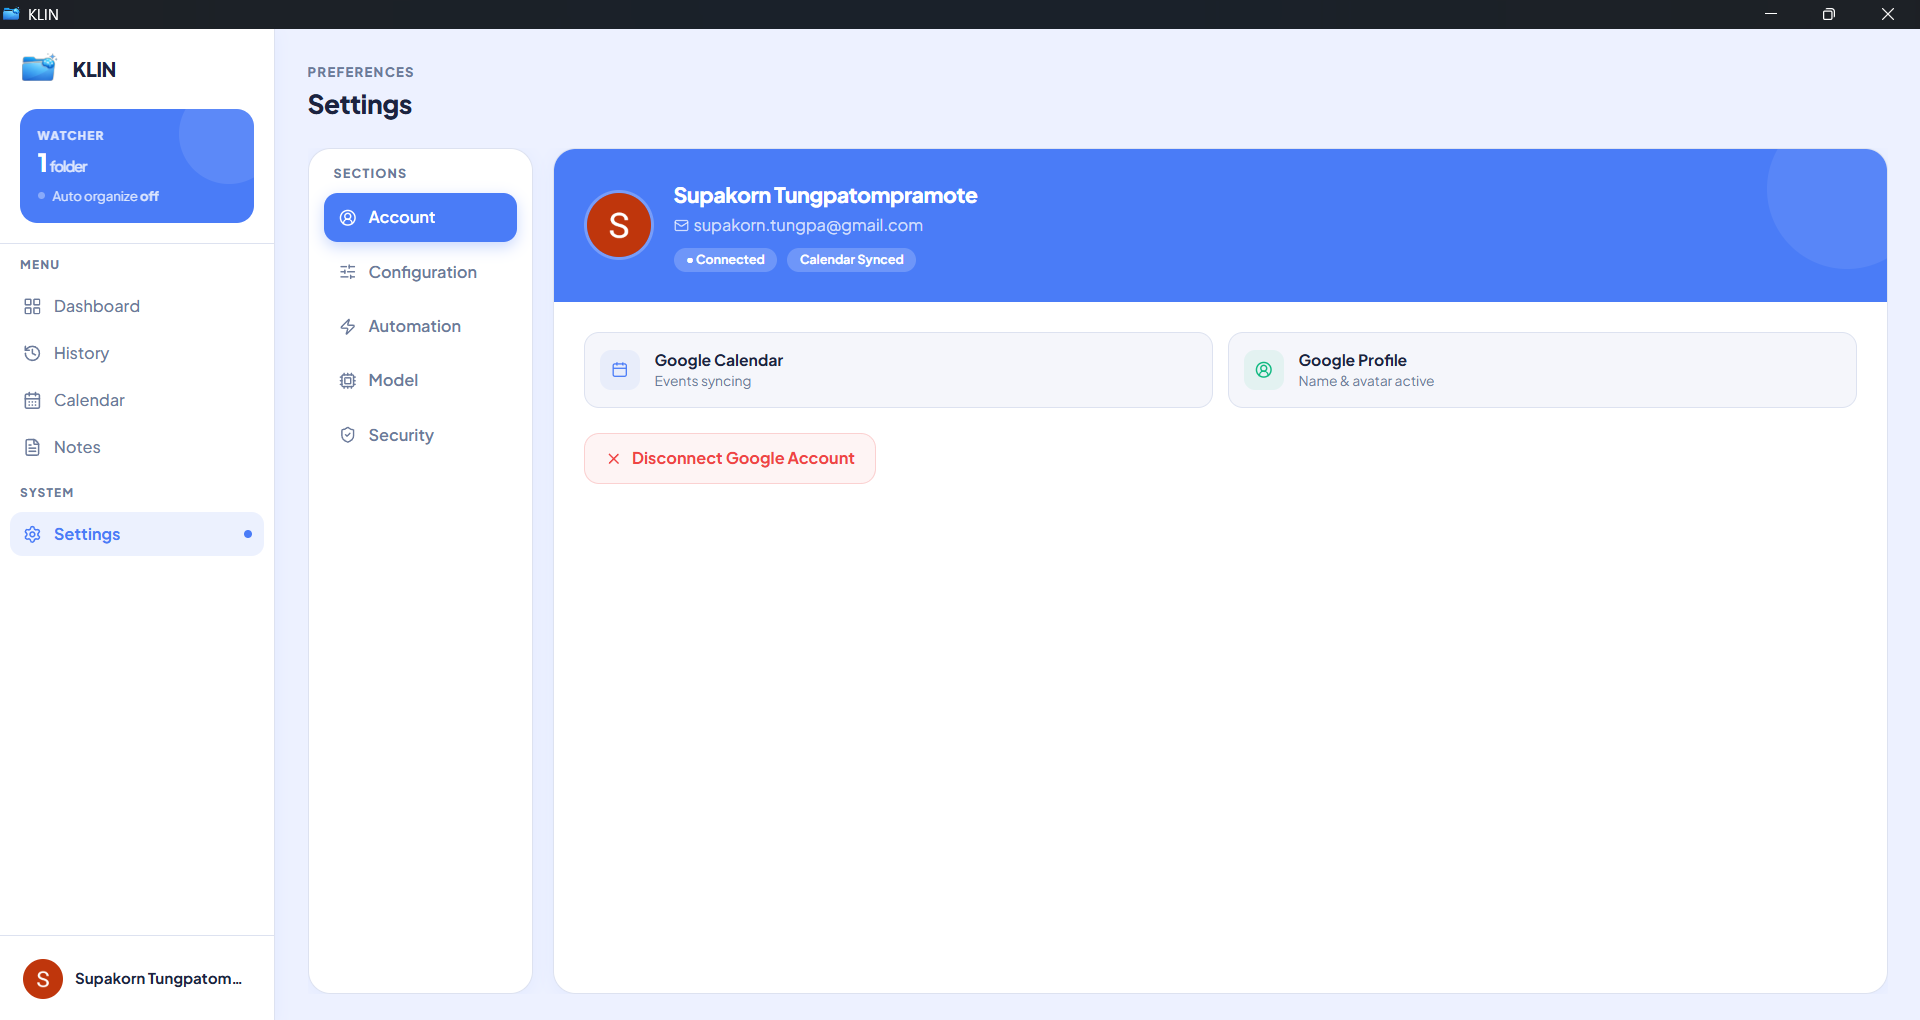
\includegraphics[width=0.9\textwidth]{figures/feature/feat_settings_account.png}
\caption{Settings -- Account: the connected Google account}
\end{figure}

\begin{figure}[H]\centering
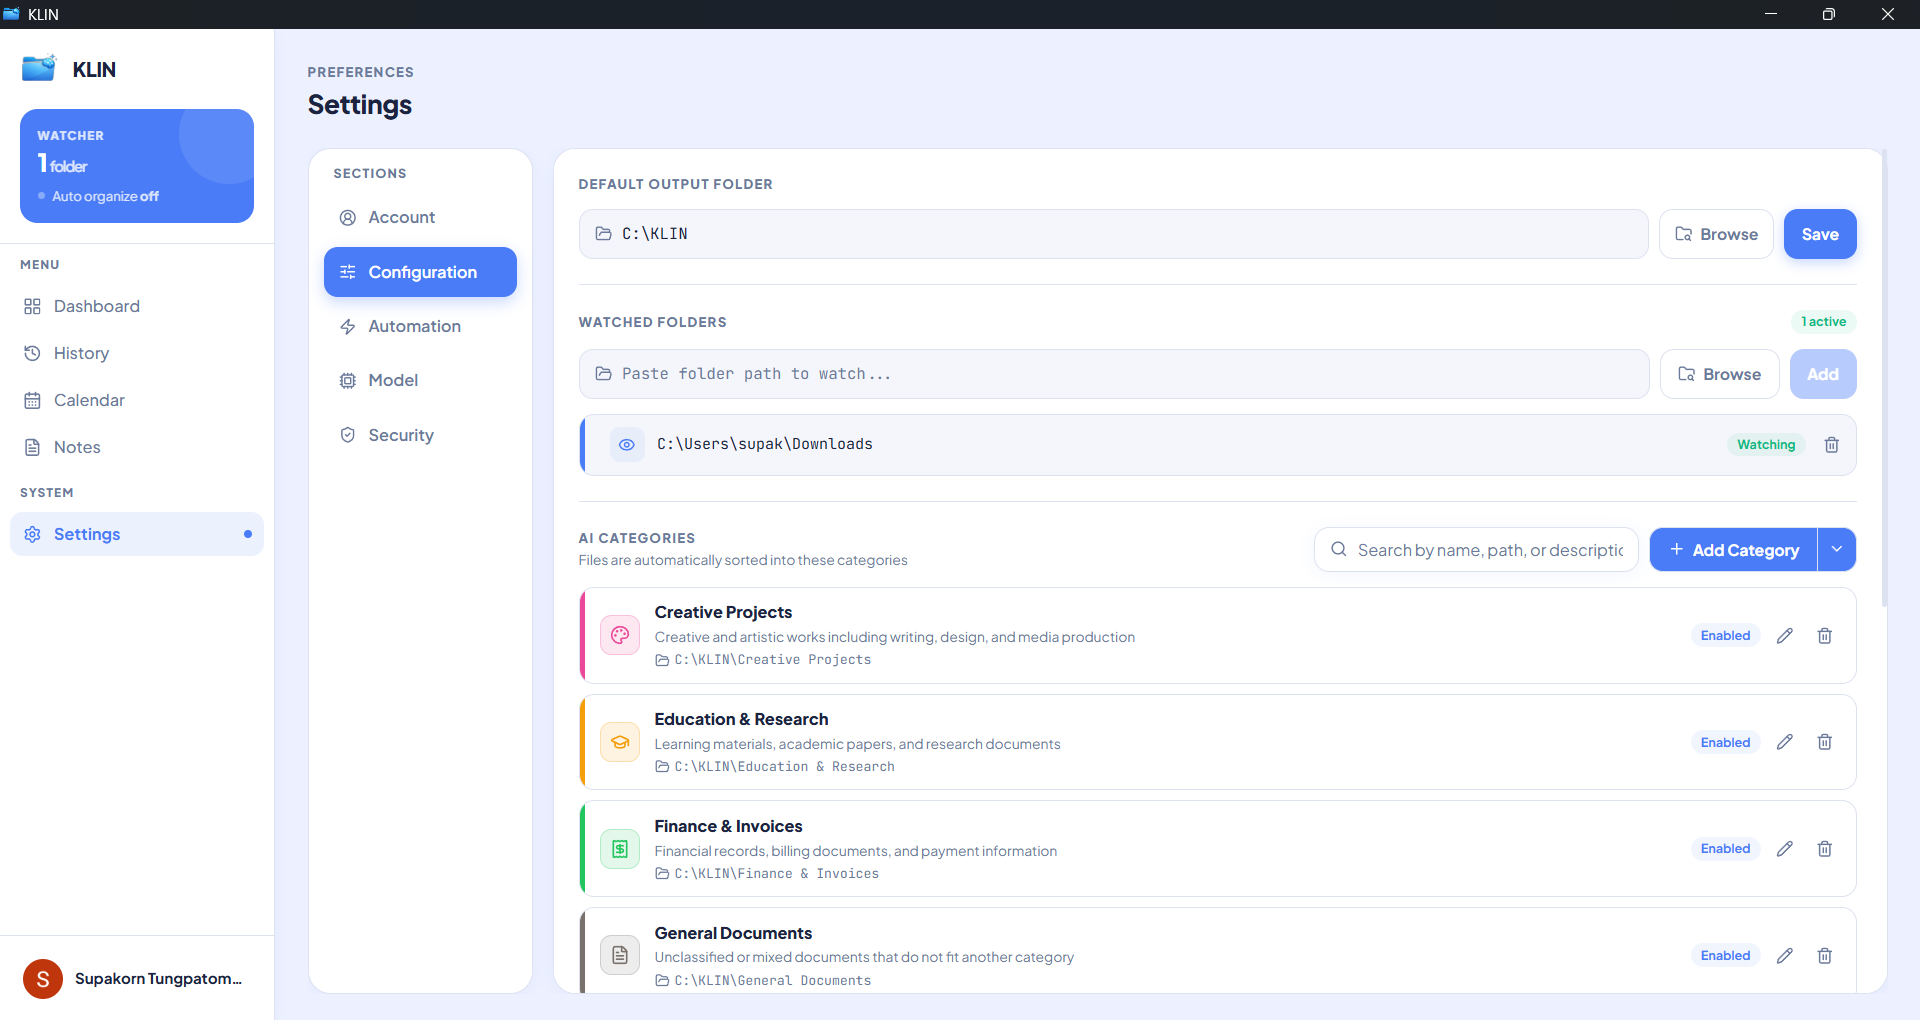
\includegraphics[width=0.9\textwidth]{figures/feature/feat_settings_config.png}
\caption{Settings -- Configuration: default output folder, watched folders, and AI categories}
\end{figure}

\begin{figure}[H]\centering
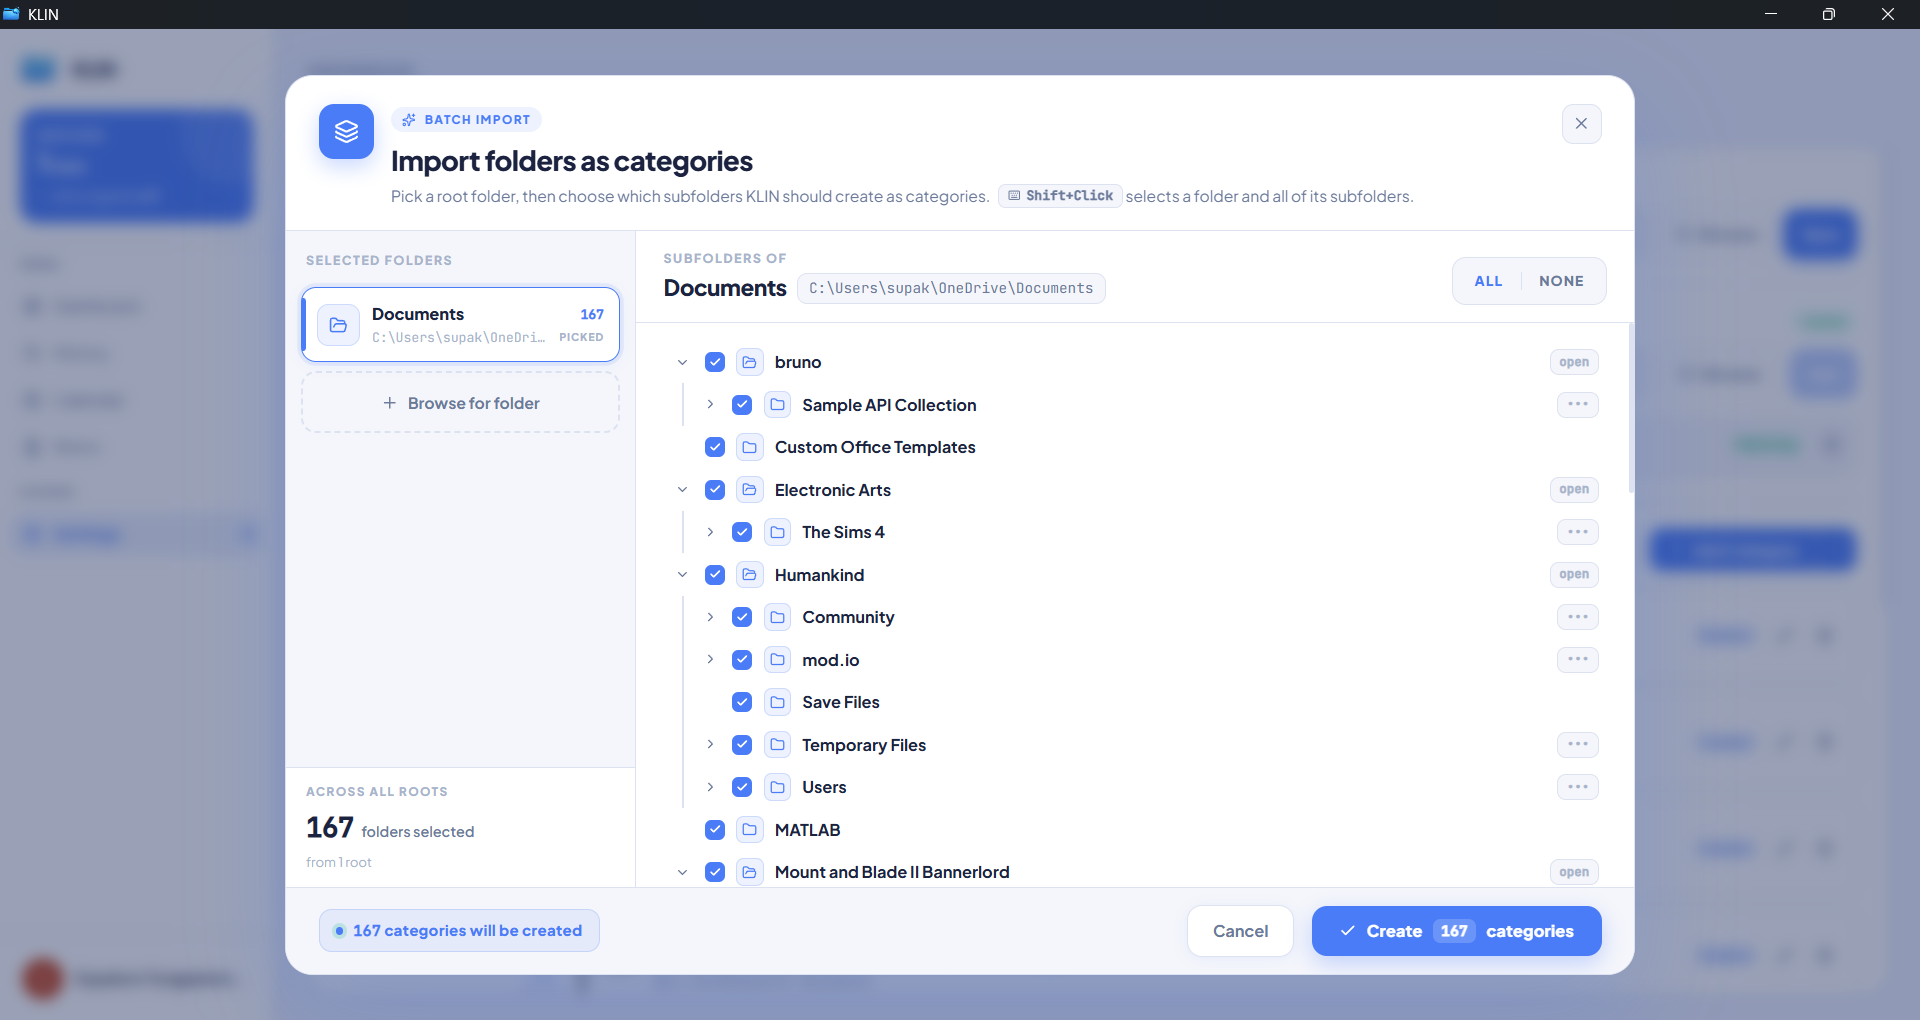
\includegraphics[width=0.9\textwidth]{figures/feature/feat_batch_category.png}
\caption{The batch import dialog, opened from the Configuration section, for importing an existing folder structure as AI categories in a single operation}
\end{figure}

\begin{figure}[H]\centering
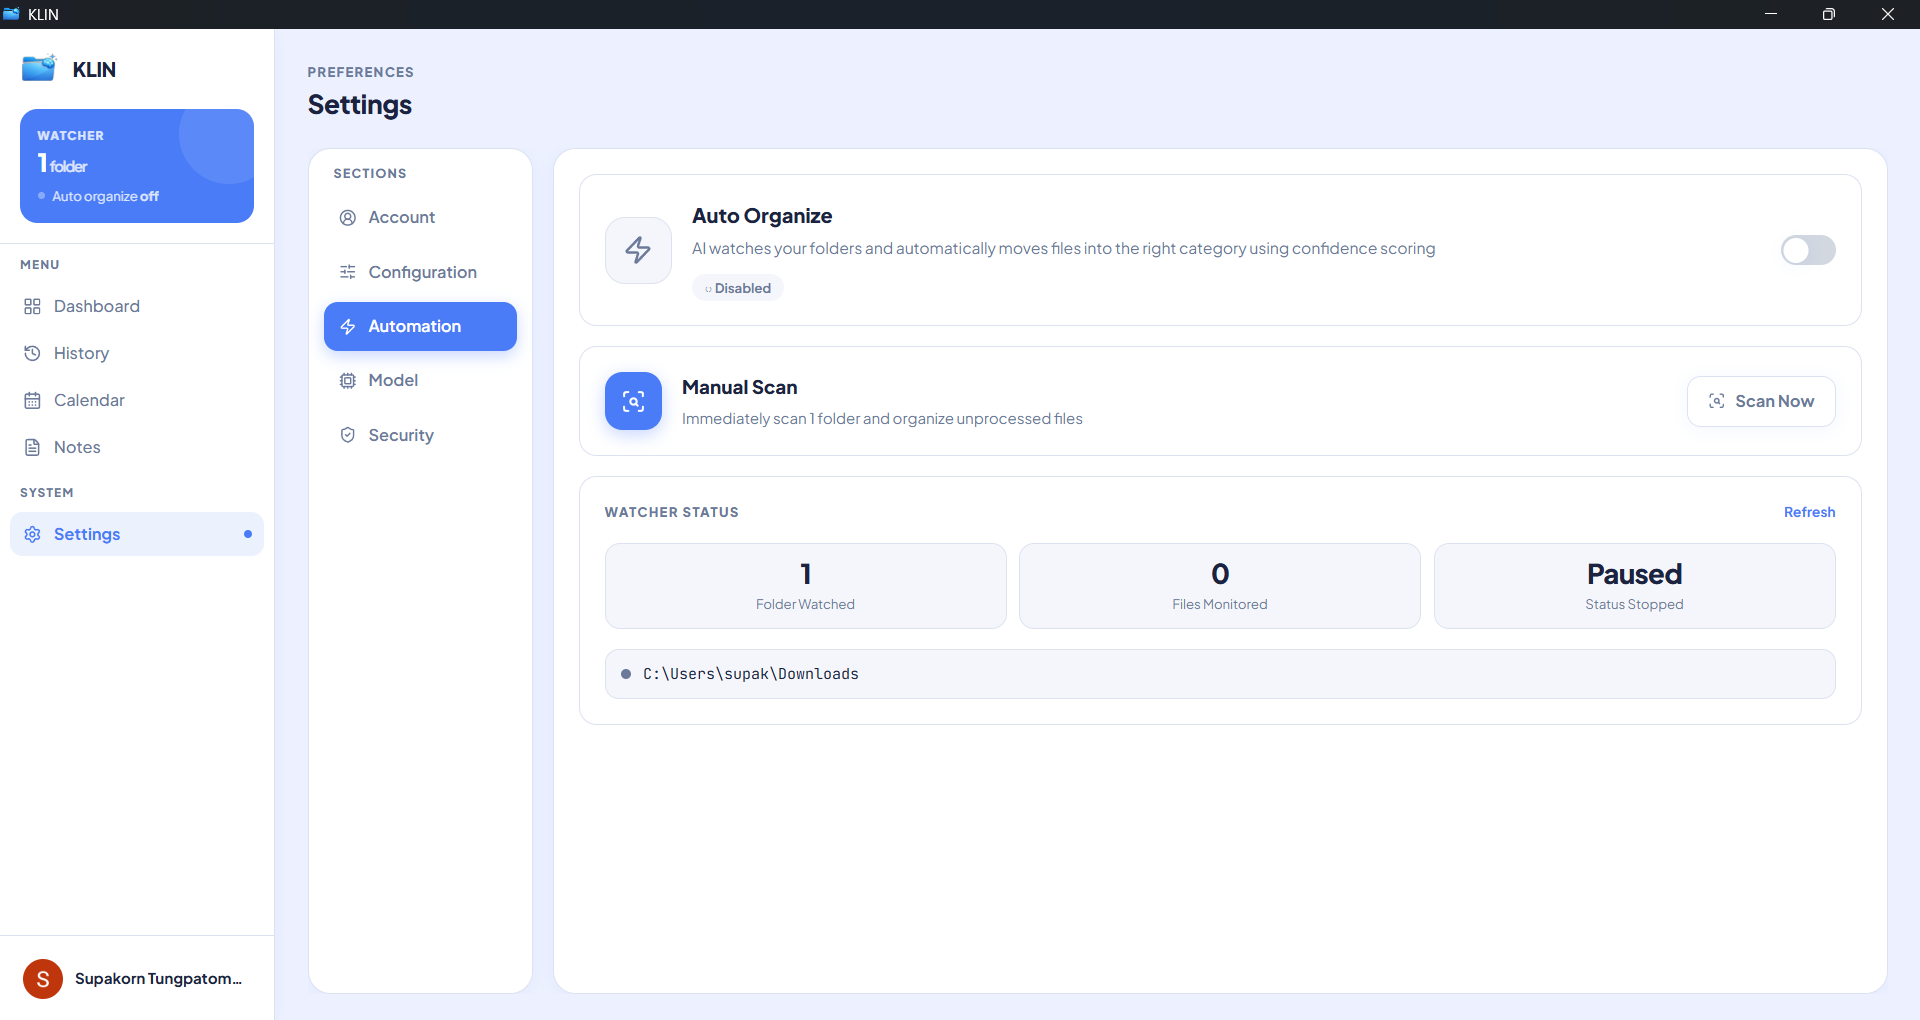
\includegraphics[width=0.9\textwidth]{figures/feature/feat_settings_automation.png}
\caption{Settings -- Automation: the Auto Organize watcher and manual scan}
\end{figure}

\begin{figure}[H]\centering
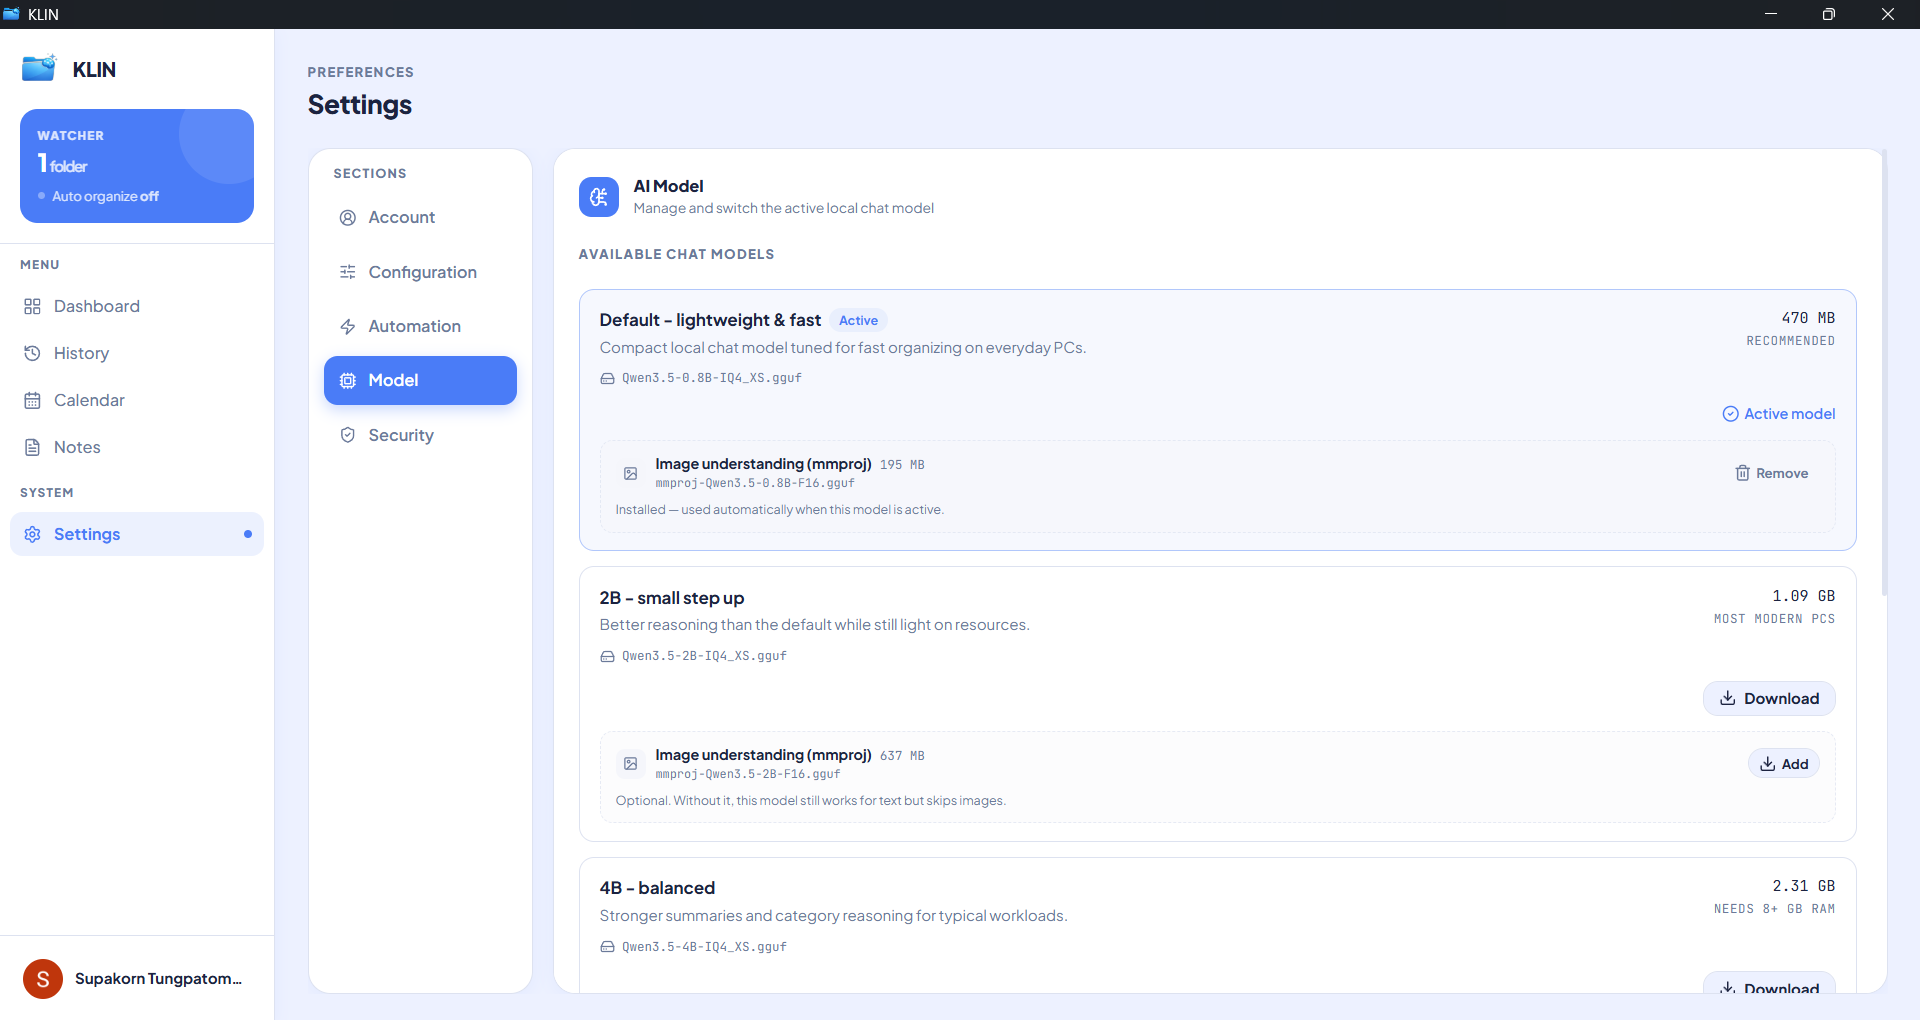
\includegraphics[width=0.9\textwidth]{figures/feature/feat_settings_model.png}
\caption{Settings -- Model: management of the local AI models}
\end{figure}

\begin{figure}[H]\centering
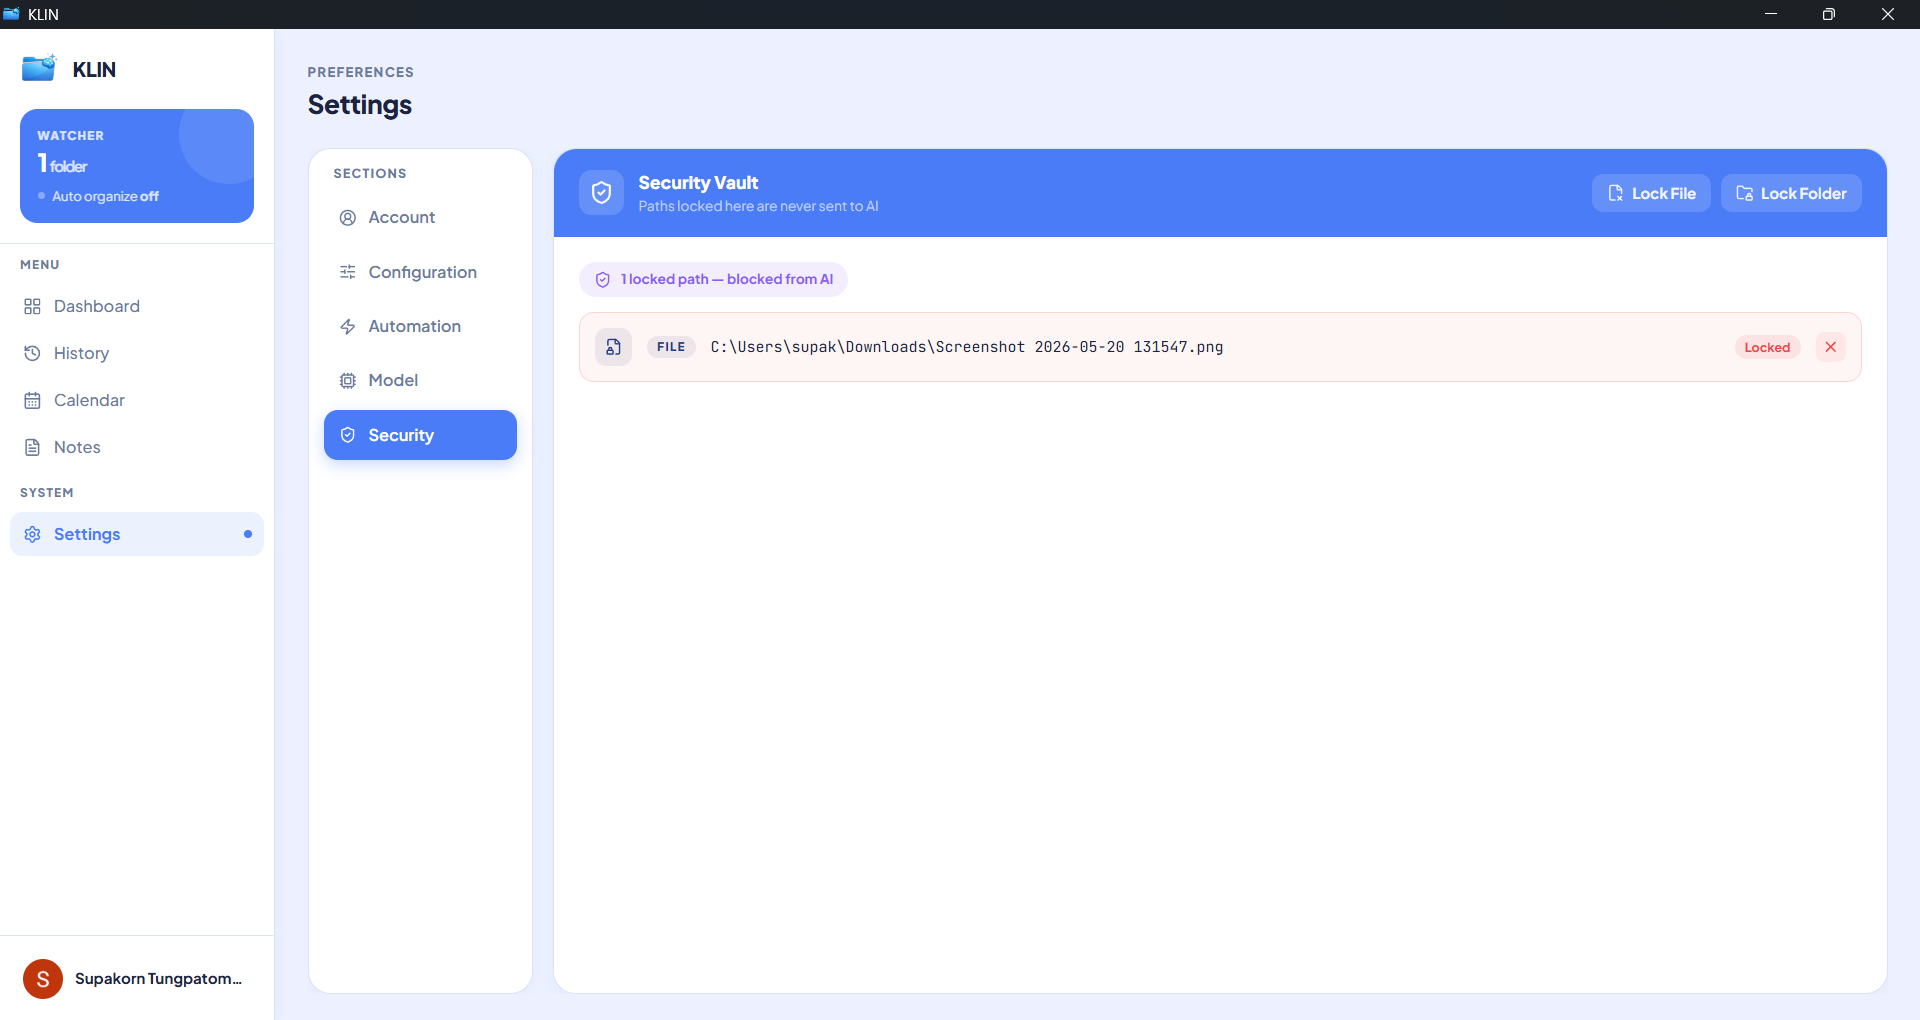
\includegraphics[width=0.9\textwidth]{figures/feature/feat_settings_security.png}
\caption{Settings -- Security: the Security Vault for locking files and folders from AI processing}
\end{figure}

\section{Automated Test Results}
In addition to the higher-level evaluations described in the following sections, an automated unit-test suite was developed alongside the source code of both the frontend and the backend. The purpose of these tests is to verify code-level correctness, to enforce the data contract shared between the two layers and to provide regression safety during ongoing development. All tests in both suites currently pass.

\subsection{Frontend Test Suite}
The frontend test suite is executed using \texttt{bun test}, Bun's built-in Jest-compatible test runner. Test files are organized in a dedicated directory at the package root, whose internal structure mirrors the \texttt{src/} hierarchy (for example, tests for \texttt{src/lib/*} live under \texttt{tests/lib/*}, and tests for \texttt{src/stores/*} live under \texttt{tests/stores/*}), and follow the \texttt{*.test.ts} naming convention. Imports use the \texttt{@/*} TypeScript path alias so each test references its module under test by the same logical path as the rest of the application code. The scope of the suite covers pure utility functions and the Zustand state stores, while React components, Tauri \texttt{invoke} calls, and end-to-end flows are intentionally not covered at this layer, as they are exercised by the persona-based benchmark and the expert evaluation. The suite contains \textbf{72 tests across 8 files} (91 assertions), all passing, with a total runtime of approximately 545~ms.

\begin{table}[H]
\centering
\caption{Frontend unit-test files and their coverage}
\begin{tabular}{|p{0.30\textwidth}|p{0.60\textwidth}|}
\hline
\textbf{Module under test} & \textbf{What it covers} \\
\hline
Category helpers & Category name normalization, matching, and defaults \\
\hline
Error helpers & Error-message extraction and error-shape normalization \\
\hline
Path helpers & Path joining, parent extraction, and separator normalization across Windows and POSIX \\
\hline
Scoring helpers & Score ranking, top-category selection, and tie handling \\
\hline
Text helpers & String formatting, truncation, and sanitization \\
\hline
General utilities & Class-name merging and other shared helpers \\
\hline
Rule store (Zustand) & Rule create, read, update, delete actions and store-state transitions \\
\hline
Undo/redo store & Undo and redo stack, history bounds, and state restoration \\
\hline
\end{tabular}
\end{table}

\subsection{Backend Test Suite}
The backend test suite is executed using \texttt{cargo test --lib}. Tests are organized in a dedicated \texttt{src/tests/} module tree whose internal structure mirrors the source hierarchy: each production module (for example \texttt{services/rule\_service.rs}) has a corresponding test file at the equivalent path under \texttt{src/tests/} (in this example \texttt{src/tests/services/rule\_service\_tests.rs}). The scope covers domain serde contracts, JSON-backed repositories (exercised against temporary directories), service-layer orchestration (exercised against in-memory fake repositories), and the sidecar idle-stop timer. The suite contains \textbf{37 tests across 9 modules}, all passing, with a total runtime of approximately 30~ms.

\begin{table}[H]
\centering
\caption{Backend unit-test modules and their coverage}
\begin{tabular}{|p{0.30\textwidth}|p{0.13\textwidth}|p{0.47\textwidth}|}
\hline
\textbf{Module under test} & \textbf{Layer} & \textbf{What it covers} \\
\hline
Domain entities & Domain & Domain-entity serialization contract and JSON round-trip encoding and decoding (prevents accidental field renames from breaking the frontend) \\
\hline
Scoring strategy & Domain & Scoring-provider identity and factory selection \\
\hline
Rule repository & Persistence & Rule persistence: missing, empty, and malformed file handling, save/list round-trip, and overwrite behavior \\
\hline
Category repository & Persistence & Category persistence: default fallback when no file exists, JSON parsing, and malformed-input error handling \\
\hline
History repository & Persistence & History-log persistence: append and list ordering, empty-file handling, and parse-error reporting \\
\hline
Automation-config repository & Persistence & Automation-config persistence: default fallback, save/load round-trip, and automatic parent-directory creation \\
\hline
Rule service & Service & Rule service orchestration: delegation to the repository and propagation of list and save errors \\
\hline
Category service & Service & Category service orchestration: pass-through to the repository, empty-result handling, and error propagation \\
\hline
History service & Service & History service orchestration: write and list ordering, and error propagation \\
\hline
Llama sidecar & Sidecar & Sidecar idle-stop timer: triggers after the timeout, holds before the timeout, and stays disabled when no activity has been recorded \\
\hline
\end{tabular}
\end{table}

\subsection{Worker Test Suite}
The worker test suite is executed using \texttt{uv run pytest -q} (pytest 9.0.2 on Python 3.13.9 in a uv-managed venv). Tests are organized under a dedicated \texttt{tests/} directory with \texttt{api/}, \texttt{services/}, \texttt{models/}, \texttt{core/}, \texttt{integration/}, and root-level tests (CLI, tracing, versioning). The suite uses pytest markers (\texttt{unit}, \texttt{integration}, \texttt{llm}) and comprehensive fakes to avoid external dependencies, including in-memory SQLite, fake RAG services, and mocked LLM calls.

At the API layer, tests cover the full set of FastAPI routes (health, organize/apply, search, summary/stream, and settings) with attention to validation errors, status-code behavior, pagination, locked-file handling, fallback paths, and SSE response formatting. Service-layer tests exercise the organize pipeline ordering and caching, schedule extraction, background ingest/RAG enqueue, LLM client behavior, classification and embedding logic, scanning safeguards, history and system log behavior, startup checks, lock settings, seed data, and telemetry. Model tests verify Pydantic request/response validators and defaults for organize, search, history, and settings payloads to keep the API contract stable. The suite contains the total of \textbf{260 tests across 37 files}, all passing, with an approximately runtime of  2.35~s.

\begin{table}[H]
\centering
\caption{Worker test areas and their coverage}
\begin{tabular}{|p{0.30\textwidth}|p{0.60\textwidth}|}
\hline
\textbf{Area} & \textbf{What it covers} \\
\hline
API routes & End-to-end behavior for \texttt{/health}, \texttt{/api/organize}+\texttt{/apply}, \texttt{/api/search}, \texttt{/api/summary}+\texttt{/stream}, and \texttt{/api/settings/*}; verifies validation errors, 2xx/4xx/5xx outcomes, locked-file short-circuiting, RAG fallback, pagination, and SSE response shape using \texttt{TestClient} with an in-memory DB \\
\hline
Services & Organize pipeline ordering and caching, schedule extraction and summary workflow, LLM client behavior (truncation, embedding validation), background ingest and RAG enqueue, classification and embeddings, scanner safeguards, history and system log, seed and startup checks, lock settings, and telemetry; all exercised with fakes and in-memory DB \\
\hline
Models & Pydantic request/response contracts: validator rules (min-length, color hex, required action), defaults for settings and pagination, and response shapes for organize, search, and history results \\
\hline
Core & AI exception helpers and config resolution \\
\hline
Integration & Cross-module pipeline behavior (prepare and enqueue) \\
\hline
Root & CLI argument parsing, tracing input capture, and version checks \\
\hline
\end{tabular}
\end{table}

\subsection{Combined Test Summary}
Across all three suites, the project has \textbf{369 automated tests in total} (72 frontend + 37 backend + 260 worker), all passing, with a combined runtime of approximately 2.9~s. The summary below consolidates the runners, conventions, and scope of each suite.

\begin{table}[H]
\centering
\caption{Combined summary of the automated test suites}
\small
\begin{tabular}{|p{0.16\textwidth}|p{0.24\textwidth}|p{0.30\textwidth}|p{0.18\textwidth}|}
\hline
 & \textbf{Frontend} & \textbf{Backend} & \textbf{Worker} \\
\hline
Runner       & \texttt{bun test} & \texttt{cargo test --lib} & \texttt{uv run pytest -q} \\
\hline
Test files   & 8 & 9 & 37 \\
\hline
Tests        & 72 & 37 & 260 \\
\hline
Result       & 72 pass / 0 fail & 37 pass / 0 fail & 260 pass / 0 fail \\
\hline
Duration     & $\sim$545~ms & $\sim$30~ms & $\sim$2.35~s \\
\hline
Style        & Separate \texttt{tests/} directory at the package root, mirroring the \texttt{src/} hierarchy; imports use the \texttt{@/*} path alias & Separate \texttt{src/tests/} module tree mirroring the source hierarchy, gated by \texttt{\#[cfg(test)] mod tests;} in \texttt{lib.rs} & Separate \texttt{tests/} directory with \texttt{api/}, \texttt{services/}, \texttt{models/}, \texttt{core/}, \texttt{integration/}, plus root tests; pytest markers for \texttt{unit}, \texttt{integration}, \texttt{llm} \\
\hline
Scope        & Pure utils + Zustand stores & Domain serde, JSON repos (with \texttt{tempfile}), services (with fake repos), sidecar idle-stop & API routes, service layer, models, core helpers, integration pipeline, CLI/tracing/version \\
\hline
Out of scope & React components, Tauri \texttt{invoke}, E2E & Tauri command handlers, fs watchers, sidecar subprocess, OAuth & Live-LLM calls and external services (Postgres, network) \\
\hline
\end{tabular}
\end{table}

\subsection{Discussion}
The automated test suites provide strong confidence in the code-level correctness of the project: the 72 frontend tests verify that the pure utility functions and Zustand stores behave as specified; the 37 backend tests verify that domain entities serialize correctly across the Tauri boundary, that JSON-backed repositories handle missing, empty, and malformed inputs safely, and that the service layer correctly delegates to and propagates errors from its repositories; and the 260 worker tests verify the FastAPI route layer, core helpers, and service pipeline behaviors using in-memory SQLite and mocked AI/RAG dependencies. The serde round-trip tests on the domain entities are particularly important, as they prevent accidental field renames from silently breaking the frontend--backend contract.

These tests, however, do not by themselves prove that the application is useful or that the end-to-end user experience is correct, and the worker suite intentionally mocks live LLM inference and external services. Component-level rendering, the live Tauri \texttt{invoke} bridge, filesystem watchers, the sidecar subprocess, and the AI classification quality are deliberately validated by the higher-level evaluations: the persona-based benchmark in Section~4.3 measures classification accuracy on realistic inputs, and the expert evaluation in Section~4.4 captures qualitative judgements about usability, security, and overall fit for real-world use. Taken together, the three layers form a complete evaluation of the project from code level up to user level.

\section{Persona-Based Benchmark Evaluation}
In addition to the expert evaluation, an automated benchmark was conducted to quantitatively measure the file classification accuracy of the ``AI-powered file organizer application'' across different real-world user profiles. This benchmark complements the expert evaluation by providing objective, reproducible measurements of the system's core classification capability.

\subsection*{Benchmark Setup}
Three user personas were defined to represent distinct document domains commonly encountered in real-world use:

\begin{itemize}
\item \textbf{Persona 1 -- Student:} test files drawn from six folders representing typical academic work (Assignments, ExamPrep, LabReports, LectureSlides, ProjectFiles, and ResearchPapers).
\item \textbf{Persona 2 -- HR Officer:} test files drawn from five folders representing common human-resources documents (EmployeeRecords, MeetingMinutes, PoliciesAndProcedures, Recruitment, and TrainingMaterials).
\item \textbf{Persona 3 -- Designer:} test files drawn from six folders representing creative-industry documents (ClientBriefs, ContractsAndProposals, InspirationAndReferences, Invoices, Portfolio, and ProjectDeliverables).
\end{itemize}

For each persona, 20 test files were prepared (60 files in total). Each file was passed to the application, which returned its top-5 ranked folder suggestions. The result for each file was then classified using the following scoring criteria:

\begin{itemize}
\item \textbf{Correct} -- the top-1 suggestion matches the correct destination folder.
\item \textbf{Almost Correct} -- the top-1 suggestion is incorrect, but the correct folder appears as the second-ranked suggestion.
\item \textbf{Incorrect} -- the correct folder appears at rank 3--5, or does not appear in the top-5 suggestions at all.
\end{itemize}

\subsection*{Benchmark Results}

\begin{figure}[H]\centering
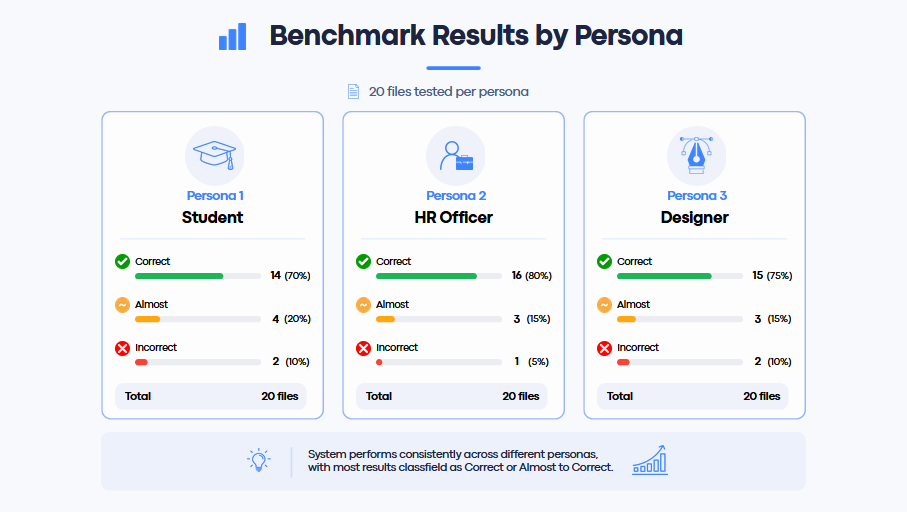
\includegraphics[width=0.9\textwidth]{figures/benchmark_personas.png}
\caption{Benchmark results by persona (20 files tested per persona)}
\end{figure}

\begin{table}[H]
\centering
\caption{Summary of benchmark results across the three personas}
\begin{tabular}{|l|c|c|c|c|}
\hline
\textbf{Persona} & \textbf{Correct} & \textbf{Almost Correct} & \textbf{Incorrect} & \textbf{Total} \\
\hline
Persona 1 -- Student     & 14 (70\%) & 4 (20\%) & 2 (10\%) & 20 \\
\hline
Persona 2 -- HR Officer  & 16 (80\%) & 3 (15\%) & 1 (5\%)  & 20 \\
\hline
Persona 3 -- Designer    & 15 (75\%) & 3 (15\%) & 2 (10\%) & 20 \\
\hline
\textbf{Overall}         & \textbf{45 (75.0\%)} & \textbf{10 (16.7\%)} & \textbf{5 (8.3\%)} & \textbf{60} \\
\hline
\end{tabular}
\end{table}

\subsection*{Analysis}
The benchmark results show that the application performs consistently across all three personas. Considering the top-1 suggestion alone, the system achieved an average accuracy of 75.0\%, with the HR Officer persona producing the highest accuracy (80\%) and the Student persona the lowest (70\%). When the ``Almost Correct'' cases are included -- that is, when the correct folder appears within the top-2 suggestions -- the combined acceptable rate rises to 91.7\% overall (90\% for Student, 95\% for HR Officer, and 90\% for Designer). Only 8.3\% of files (5 of 60) fell into the Incorrect category.

These results indicate that the system generalizes well across document domains with very different vocabulary and structure, from academic papers to HR policy documents to creative client briefs. The slightly lower accuracy on the Student persona can be attributed to overlapping content between related academic folders (for example, lab reports and project files often share similar terminology), while HR documents tend to use more distinctive domain-specific vocabulary that the model classifies more reliably. Overall, the benchmark supports the expert evaluation findings and confirms that the application's classification capability is suitable for practical, real-world use across diverse user profiles.

\section{Expert Evaluation Form}

The Evaluation tool used to evaluate the application was a performance evaluation form, which will be filled by 3 experts from the field of computer engineering or software development, can be divided into two sections:

\vspace{0.5em}

Part 1: Performance evaluation of the ``AI-powered file organizer application'' by experts. The project developers defined a 5-point scoring scale with the following meanings:

\begin{enumerate}[label=\arabic*.,leftmargin=0.6in]
\item : unable to solve the problem.
\item : able to solve the problem partially, but some gaps remain.
\item : able to solve the problem appropriately, but further improvement is still possible
\item : able to solve the problem effectively with minor improvements possible.
\item : able to solve the problem completely and appropriately.
\end{enumerate}
Part 2: Additional comments and suggestions on the performance evaluation of the ``AI-powered file organizer application''

\subsection*{The data analysis in this project was conducted using computer software packages. The statistics used for analysis were as follows:}
Data from the performance evaluation form of the ``AI-powered file organizer application'' were analyzed using the mean ( X ) and standard deviation ( S.D. ). The interpretation of the mean scores was defined as follows (Boonchom Srisa-ard, 2002: 162):

\vspace{1em}

Mean score between 4.51 -- 5.00 means able to solve the problem completely and appropriately.

Mean score between 3.51 -- 4.50 means able to solve the problem effectively with minor improvements possible.

Mean score between 2.51 -- 3.50 means able to solve the problem appropriately, but further improvement is still possible.

Mean score between 1.51 -- 2.50 means able to solve the problem partially, but some gaps remain.

Mean score between 1.00 -- 1.50 means unable to solve the problem.

\subsection*{Data Analysis}
The project developers analyzed data from the expert performance evaluation form for the ``AI-powered file organizer application''. The evaluation was conducted by 3 experts. The analysis results were presented in tables together with descriptive explanations and divided into two parts as follows:

Part 1: Analysis results of the expert performance evaluation of the ``AI-powered file organizer application''. The analysis used the mean and standard deviation, both overall and by individual evaluation items. To make the data analysis easier to understand, the developer defined the statistical symbols and abbreviations used in the study as follows:

\noindent\hspace*{0.6in} n refers to the sample size.

\noindent\hspace*{0.6in} X refers to the mean score of satisfaction.

\noindent\hspace*{0.6in} ( S.D. ) refers to the standard deviation.

Part 2: Additional comments and suggestions on the performance evaluation of the ``AI-powered file organizer application''.

\subsection*{Data Analysis Results}
Part 1: Analysis results of the expert performance evaluation of the ``AI-powered file organizer application'' using the mean and standard deviation, both overall and by individual evaluation items.

\begin{longtable}{|p{0.52\textwidth}|p{0.10\textwidth}|p{0.10\textwidth}|p{0.16\textwidth}|}
\caption{Mean, standard deviation, and analysis of expert opinions regarding the performance of the ``AI-powered file organizer application''}\\
\hline
\multirow{2}{*}{\textbf{Evaluation Items}} & \multicolumn{3}{c|}{\textbf{Result}} \\
\cline{2-4}
 & \textbf{X} & \textbf{SD} & \textbf{Interpretation} \\
\hline
\endfirsthead
\hline
\textbf{Evaluation Items} & \textbf{X} & \textbf{SD} & \textbf{Interpretation} \\
\hline
\endhead
1. The system can accurately read and analyze data from PDF, Word, Excel, PowerPoint, TXT, and image files. & 4.33 & 0.57 & ( 4 ) \\
\hline
2. The system can accurately and appropriately categorize files based on their content. & 3.66 & 0.47 & ( 4 ) \\
\hline
3. The system can accurately and appropriately move files to destination folders according to defined templates. & 5 & 0 & ( 5 ) \\
\hline
4. The Preview system effectively helps reduce errors before moving or modifying files. & 5 & 0 & ( 5 ) \\
\hline
5. The history recording and Undo/Redo system is appropriate for practical use. & 4 & 0 & ( 4 ) \\
\hline
6. The UI design is easy to learn and use. & 3.51 & 0.47 & ( 4 ) \\
\hline
7. AI-related features, such as content summarization, note generation, and search are appropriate for practical use. & 4 & 0 & ( 4 ) \\
\hline
8. The system provides appropriate measures to prevent risks to user data. & 5 & 0 & ( 5 ) \\
\hline
9. The overall system architecture is appropriate for development as a desktop application. & 4 & 0 & ( 4 ) \\
\hline
10. The system has the potential to support real-world use on Windows. & 4.66 & 0.47 & ( 5 ) \\
\hline
\textbf{Total} & \textbf{4.31} & \textbf{0.19} & \textbf{( 4 )} \\
\hline
\end{longtable}

From Table 4.1, it was found that the experts' opinions regarding the performance of the ``AI-powered file organizer application'' were overall at the level of able to solve the problem effectively with minor improvements possible, with a mean score of 4.31. The standard deviation was 0.19, indicating a low level of dispersion from the mean. This means that the experts' opinions regarding the application's performance were similar and consistent. And when considering each evaluation item individually, four items were rated at the level of able to solve the problem completely and appropriately. These items were: The system can accurately and appropriately move files to destination folders according to defined templates, The Preview system effectively helps reduce errors before moving or modifying files, The system provides appropriate measures to prevent risks to user data, The system has the potential to support real-world use on Windows. The remaining evaluation items were rated at the level of able to solve the problem effectively with minor improvements possible.

\bigskip
\noindent\textbf{Part 2: Additional Comments and Suggestions on the Performance Evaluation of the ``AI-powered file organizer application''}

\bigskip
\noindent\textbf{Expert 1} evaluated that this application is of very good quality. This reflects a clear understanding of applying a Local LLM to solve real-world problems. The application has several strengths, including:

\subsection*{Strengths}
\begin{itemize}
\item Use of Offline AI (llama.ccp) -- This is an important strength, especially for organizations that require privacy and do not want to rely on cloud services.
\item Preview \& Undo System -- This is very well designed and helps reduce the risk of incorrect file organization. It also provides good user experience.
\item Full Thai Language Support -- The system supports Thai documents, showing attention to the local context.
\item Hybrid Approach (Keyword + AI) -- Using keyword matching first and then sending the task to AI is a good concept. It helps save time and computational resources.
\end{itemize}
\subsection*{Areas for Improvement}
\begin{itemize}
\item UI/UX -- Although the application is usable, it is recommended to further study Material Design or Fluent Design, and Dark Mode may also be considered.
\item Error Handling -- Error handling should be clearer. For example, if AI models are not running or some process fails, the system should display easy-to-understand messages.
\item Documentation -- A complete user manual should be provided, including a troubleshooting guide.
\end{itemize}
\subsection*{Additional Suggestions}
\begin{itemize}
\item Consider adding an adjustable Confidence Score Threshold for users, such as asking the user for confirmation if the AI confidence score is lower than 70\%.
\item Add a Batch Rename feature to rename files according to a predefined format.
\end{itemize}
\subsection*{Overall Comment}
This application has academic value and can be applied in real-world use. It is recommended that the project be further developed as an Open-Source Project. The developers may also consider publishing a paper on the Hybrid Keyword-AI Approach for Thai-language documents.

\bigskip
\noindent\textbf{Expert 2} evaluated that this ``AI-powered file organizer application'' is highly outstanding and useful, especially in educational and real-world working contexts.

\subsection*{Strengths}
\begin{itemize}
\item Practical Usability -- This is not only a sample project, but an application that can be immediately used to solve real problems in offices or government agencies, where large numbers of documents often need to be organized.
\item Thai document parsing -- This is a major strength because most government documents are in Thai and often include scanned documents that require OCR. The ability to support Thai language well makes the application practical for real use.
\item 100\% Offline Operation -- This is very important for organizations that handle sensitive information, as they do not need to worry about data security risks from cloud services.
\item Preview and Undo Features -- Students often develop projects without considering these features, but this project clearly takes real users into account.
\end{itemize}
\subsection*{Application in Teaching}
This project is a very good example for students to learn from in the following areas:

\begin{itemize}
\item Machine Learning Integration -- It demonstrates integration with the AI models.
\item File Handling -- It involves managing multiple file formats.
\item Real-World Problem Solving -- It solves a real problem rather than simply following a basic example.
\end{itemize}
\subsection*{Areas for Improvement}
\begin{itemize}
\item Create Tutorial Videos -- Tutorial videos should be created to help general users understand how to use the application more quickly, especially users who are not familiar with technology.
\item Improve the UI for Easier Use -- Although the application is already usable, it should include a wizard or guided setup for first-time users.
\item Add Use Case Examples -- Preset templates should be provided, such as ``organizing human resources documents'' or ``organizing financial documents.''
\end{itemize}
\subsection*{Additional Suggestions}
\begin{itemize}
\item Consider adding multi-language support, starting with Thai and English, which has already been implemented, and possibly adding more languages in the future.
\item Add Export/Import Settings so that users can share templates with their colleagues.
\item Develop a Lite Version for low-specification computers, which may use only keyword matching without AI.
\end{itemize}
\subsection*{Overall Comment}
This ``AI-powered file organizer application'' is highly suitable for presentation at an academic conference. It should also be considered for release as an Open-Source Project so that the community can benefit from it. This would also help build recognition for the institution and the developers.

\bigskip
\noindent\textbf{Expert 3} evaluated this application from the perspective of real-world organizational use and data security.

\subsection*{Strengths}
\begin{itemize}
\item Offline-first Architecture -- Data does not leave the user's device, making it suitable for organizations that handle sensitive information.
\item Local AI Processing -- This helps reduce the risk of data breaches.
\item Password-protected File Support -- The application takes data security into consideration.
\item System Architecture -- The code structure is well organized, and the installer is ready for use.
\end{itemize}
\subsection*{Areas for Improvement for Enterprise Deployment}
\begin{itemize}
\item Security and Access Control -- User authentication and role-based access control should be added for organizational use.
\item Audit Trail -- Logs should include more details, such as User ID, IP address, and file hash for integrity checking.
\item Scalability -- A database such as SQLite should be considered instead of JSON files when handling a large number of files.
\item Network Deployment -- A client-server architecture should be developed to allow multiple users to work together more conveniently.
\item Backup and Recovery -- Auto-backup mechanisms for configuration and export/import settings should be provided.
\end{itemize}
\subsection*{Additional Suggestions}
\begin{itemize}
\item Consider Active Directory integration for organizations using a Windows Domain.
\item Add API endpoints so that other systems can access and use the application.
\item Develop a Health Check Dashboard for IT administrators to monitor system status.
\end{itemize}
\subsection*{Overall Comment}
The application has a very strong foundation and is ready for personal use or small teams. However, if it is intended for use in large organizations, additional enterprise features should be developed according to the suggestions above. The use of Offline AI is an important strength in the on-premises solution market.

\chapter{Conclusion and Recommendations}
The project titled ``AI-powered file organizer application'' can be summarized, discussed, and presented with recommendations as follows:

\section{Project Summary}
\subsection*{Project Objectives}
\begin{itemize}
\item To develop a desktop application that helps users manage files efficiently with AI.
\item To reduce repetitive tasks and errors caused by manual file management.
\item To improve the convenience of searching and organizing files through customizable file management templates.
\item To establish a foundation for future expansion toward Agentic AI features, such as file content summarization, note generation, and calendar integration.
\end{itemize}
\section{Methodology}
\subsection*{Expert Evaluation tool for Application Performance}

The Evaluation tool used to evaluate the application was a performance evaluation form, which will be filled by 3 experts from the field of computer engineering or software development, can be divided into two sections:

\vspace{0.5em}

Part 1: Performance evaluation of the ``AI-powered file organizer application'' by experts. The project developers defined a 5-point scoring scale with the following meanings:

\begin{enumerate}[label=\arabic*.,leftmargin=0.6in]
\item : unable to solve the problem.
\item : means able to solve the problem partially, but some gaps remain.
\item : means able to solve the problem appropriately, but further improvement is still possible
\item : means able to solve the problem effectively with minor improvements possible.
\item : means able to solve the problem completely and appropriately.
\end{enumerate}
Part 2: Additional comments and suggestions on the performance evaluation of the ``AI-powered file organizer application''

\subsection*{The data analysis in this project was conducted using computer software packages. The statistics used for analysis were as follows:}
Data from the performance evaluation form of the ``AI-powered file organizer application'' were analyzed using the mean ( X ) and standard deviation ( S.D. ). The interpretation of the mean scores was defined as follows (Boonchom Srisa-ard, 2002: 162):

\vspace{1em}

Mean score between 4.51 -- 5.00 means able to solve the problem completely and appropriately.

Mean score between 3.51 -- 4.50 means able to solve the problem effectively with minor improvements possible.

Mean score between 2.51 -- 3.50 means able to solve the problem appropriately, but further improvement is still possible.

Mean score between 1.51 -- 2.50 means able to solve the problem partially, but some gaps remain.

Mean score between 1.00 -- 1.50 means unable to solve the problem.
\vspace{1ex}

The result from the Expert Evaluation from stated that the experts' opinions regarding the performance of the ``AI-powered file organizer application'' were overall at the level of able to solve the problem effectively with minor improvements possible, with a mean score of 4.31. The standard deviation was 0.19, indicating a low level of dispersion from the mean. This means that the experts' opinions regarding the application's performance were similar and consistent. And when considering each evaluation item individually, four items were rated at the level of able to solve the problem completely and appropriately. These items were: The system can accurately and appropriately move files to destination folders according to defined templates, The Preview system effectively helps reduce errors before moving or modifying files, The system provides appropriate measures to prevent risks to user data, The system has the potential to support real-world use on Windows. The remaining evaluation items were rated at the level of able to solve the problem effectively with minor improvements possible.

\subsection*{Summary of Expert Opinions on the Performance Evaluation of the ``AI-powered file organizer application''}
\begin{itemize}
\item This application has academic value and can be applied in real-world use. It is recommended that the project be further developed as an Open-Source Project. The developers may also consider publishing a paper on the Hybrid Keyword-AI Approach for Thai-language documents.
\item This ``AI-powered file organizer application'' is highly suitable for presentation at an academic conference. It should also be considered for release as an Open-Source Project so that the community can benefit from it. This would also help build recognition for the institution and the developers.
\item The application has a very strong foundation and is ready for personal use or small teams. However, if it is intended for use in large organizations, additional enterprise features should be developed according to the suggestions above. The use of Offline AI is an important strength in the on-premises solution market.
\end{itemize}
\section{Project Recommendations}
\begin{enumerate}[label=\arabic*.,leftmargin=0.6in]
\item Consider adding an adjustable Confidence Score Threshold, such as asking the user for confirmation if the AI confidence score is lower than 70\%.
\item Add a Batch Rename feature to rename files according to a predefined format.
\item Consider adding Multi-language Support, starting with Thai and English, which has already been implemented, and possibly adding more languages in the future.
\item Add Export/Import Settings so that users can share templates with their colleagues.
\item Develop a Lite Version for low-specification computers, which may use only keyword matching without AI.
\item Consider Active Directory Integration for organizations using a Windows Domain.
\item Add API Endpoints so that other systems can access and use the application.
\item Develop a Health Check Dashboard for IT administrators to monitor system status.
\end{enumerate}

\section{Future Work}
In addition to the short-term recommendations listed above, there are four longer-term directions for the future of the project. These are larger in scope than the recommendations above, each one introduces a new capability, new architectural component, or a new class of file. Therefore, it is presented separately as future-work items rather than as immediate suggestions.

\subsection*{1. Expanded File-Type Support}
Extension support for audio files (such as MP3 and WAV) and video files (such as MP4 and MOV), which are increasingly common in personal and professional file libraries. This extension would allow the application to organize a much wider range of real-world file types and covering more in user's need.

\subsection*{2. Semantic and Contextual Image Understanding}
The current image-classification capability operates primarily at the object level, recognizing concepts such as ``a cat'', ``a dog'', or ``a person.'' A more powerful future capability is scene-level and event-level understanding for example, recognizing that a set of photographs depicts ``a travel trip with friends in front of historical architecture'' rather than merely ``people and buildings.'' This kind of contextual interpretation would allow the application to group personal photo libraries by meaningful events (trips, ceremonies, projects) instead of by isolated objects. The main constraint today is the size and capability of vision-language models that can run fully on-device under the project's offline-first requirement. As smaller, more capable VLMs continue to be released, this capability is expected to become practical to integrate without compromising the local-only architecture.

\subsection*{3. Parallel and Concurrent File Indexing}
The current file-indexing pipeline processes files largely in sequence. A future direction is to enable parallel and concurrent indexing so that the application can handle large libraries with much shorter scan times. The intention is to keep performance smooth and the user interface responsive as the collection grows, without changing the user-facing workflow.

\subsection*{4. Large-Folder Handling}
When a single folder contains a very large number of files, reading it will bring problem or takes too long especially in auto-organzing. The solution is to revise the scanning function to handle pagination or chunking the files first, while also preserving or better the performance of the feature. This will allow the application to work well even with folders containing tens of thousands of files, which is common in real-world use cases such as photo libraries or project archives.

\chapter*{REFERENCES}\addcontentsline{toc}{chapter}{REFERENCES}
\begin{enumerate}[label=\arabic*.,leftmargin=0.6in]
\item AWS, 2024, ``What is Natural Language Processing (NLP)? - AWS,'' Available at \url{https://aws.amazon.com/th/what-is/nlp/}, [Online; accessed 4-May-2026].
\item AWS, 2024, ``What is LLM? - Large Language Model Explanation - AWS,'' Available at \url{https://aws.amazon.com/th/what-is/large-language-model/}, [Online; accessed 4-May-2026].
\item NVIDIA, 2024, ``What are Vision-Language Models? | NVIDIA Glossary,'' Available at \url{https://www.nvidia.com/en-us/glossary/vision-language-models/}, [Online; accessed 4-May-2026].
\item AWS, 2024, ``What is Retrieval-Augmented Generation (RAG)? - AWS,'' Available at \url{https://aws.amazon.com/th/what-is/retrieval-augmented-generation/}, [Online; accessed 4-May-2026].
\item Ollama, 2026, ``Ollama,'' Available at \url{https://ollama.com/}, [Online; accessed 4-May-2026].
\item Hugging Face, 2026, ``Hugging Face -- The AI community building the future,'' Available at \url{https://huggingface.co/}, [Online; accessed 4-May-2026].
\item Z. Guo, X. Ren, L. Xu, J. Zhang, and C. Huang, 2025, ``RAG-Anything: All-in-One RAG Framework,'' arXiv:2510.12323 [cs.AI], Oct. 2025. Available at \url{https://arxiv.org/abs/2510.12323}, [Online; accessed 4-May-2026].
\item HKUDS, 2026, ``GitHub - HKUDS/RAG-Anything: 'RAG-Anything: All-in-One RAG Framework','' Available at \url{https://github.com/HKUDS/RAG-Anything}, [Online; accessed 4-May-2026].
\item HKUDS, 2026, ``GitHub - HKUDS/LightRAG: [EMNLP2025] 'LightRAG: Simple and Fast Retrieval-Augmented Generation','' Available at \url{https://github.com/HKUDS/LightRAG}, [Online; accessed 4-May-2026].
\item Python Software Foundation, 2026, ``Our Documentation | Python.org,'' Available at \url{https://www.python.org/doc/}, [Online; accessed 4-May-2026].
\item The Rust Project Developers, 2018, ``Documentation - The Rust Programming Language - MIT,'' Available at \url{https://web.mit.edu/rust-lang_v1.25/arch/amd64_ubuntu1404/share/doc/rust/html/book/first-edition/documentation.html}, [Online; accessed 4-May-2026].
\item Tauri, 2026, ``Create a Project - Tauri,'' Available at \url{https://v2.tauri.app/start/}, [Online; accessed 4-May-2026].
\item D.K. Gifford, P. Jouvelot, M.A. Sheldon, and J.W. O'Toole Jr., 1991, ``Semantic File Systems,'' in Proc. 13th ACM Symposium on Operating Systems Principles, pp. 16--25, Oct. 1991. Available at \url{https://pages.cs.wisc.edu/~remzi/Classes/838/Fall2001/Papers/sfs-sosp91.pdf}, [Online; accessed 4-May-2026].
\item N. Sengar, R.C. Joshi, and M.K. Dutta, 2023, ``Auto Organizer: A Machine Learning-Based Tool for Automatic Organization of Files,'' Lecture Notes in Electrical Engineering, Jun. 2023. Available at \url{https://www.researchgate.net/publication/371930502_Auto_Organizer_A_Machine_Learning-Based_Tool_for_Automatic_Organization_of_Files}, [Online; accessed 4-May-2026].
\item ggml-org, 2026, ``ggml-org/llama.cpp: LLM inference in C/C++ - GitHub,'' Available at \url{https://github.com/ggml-org/llama.cpp}, [Online; accessed 4-May-2026].
\end{enumerate}

\appendix{Experts' form}
% Expert 1: ผศ.ดร.แสงอุทัย มอโท
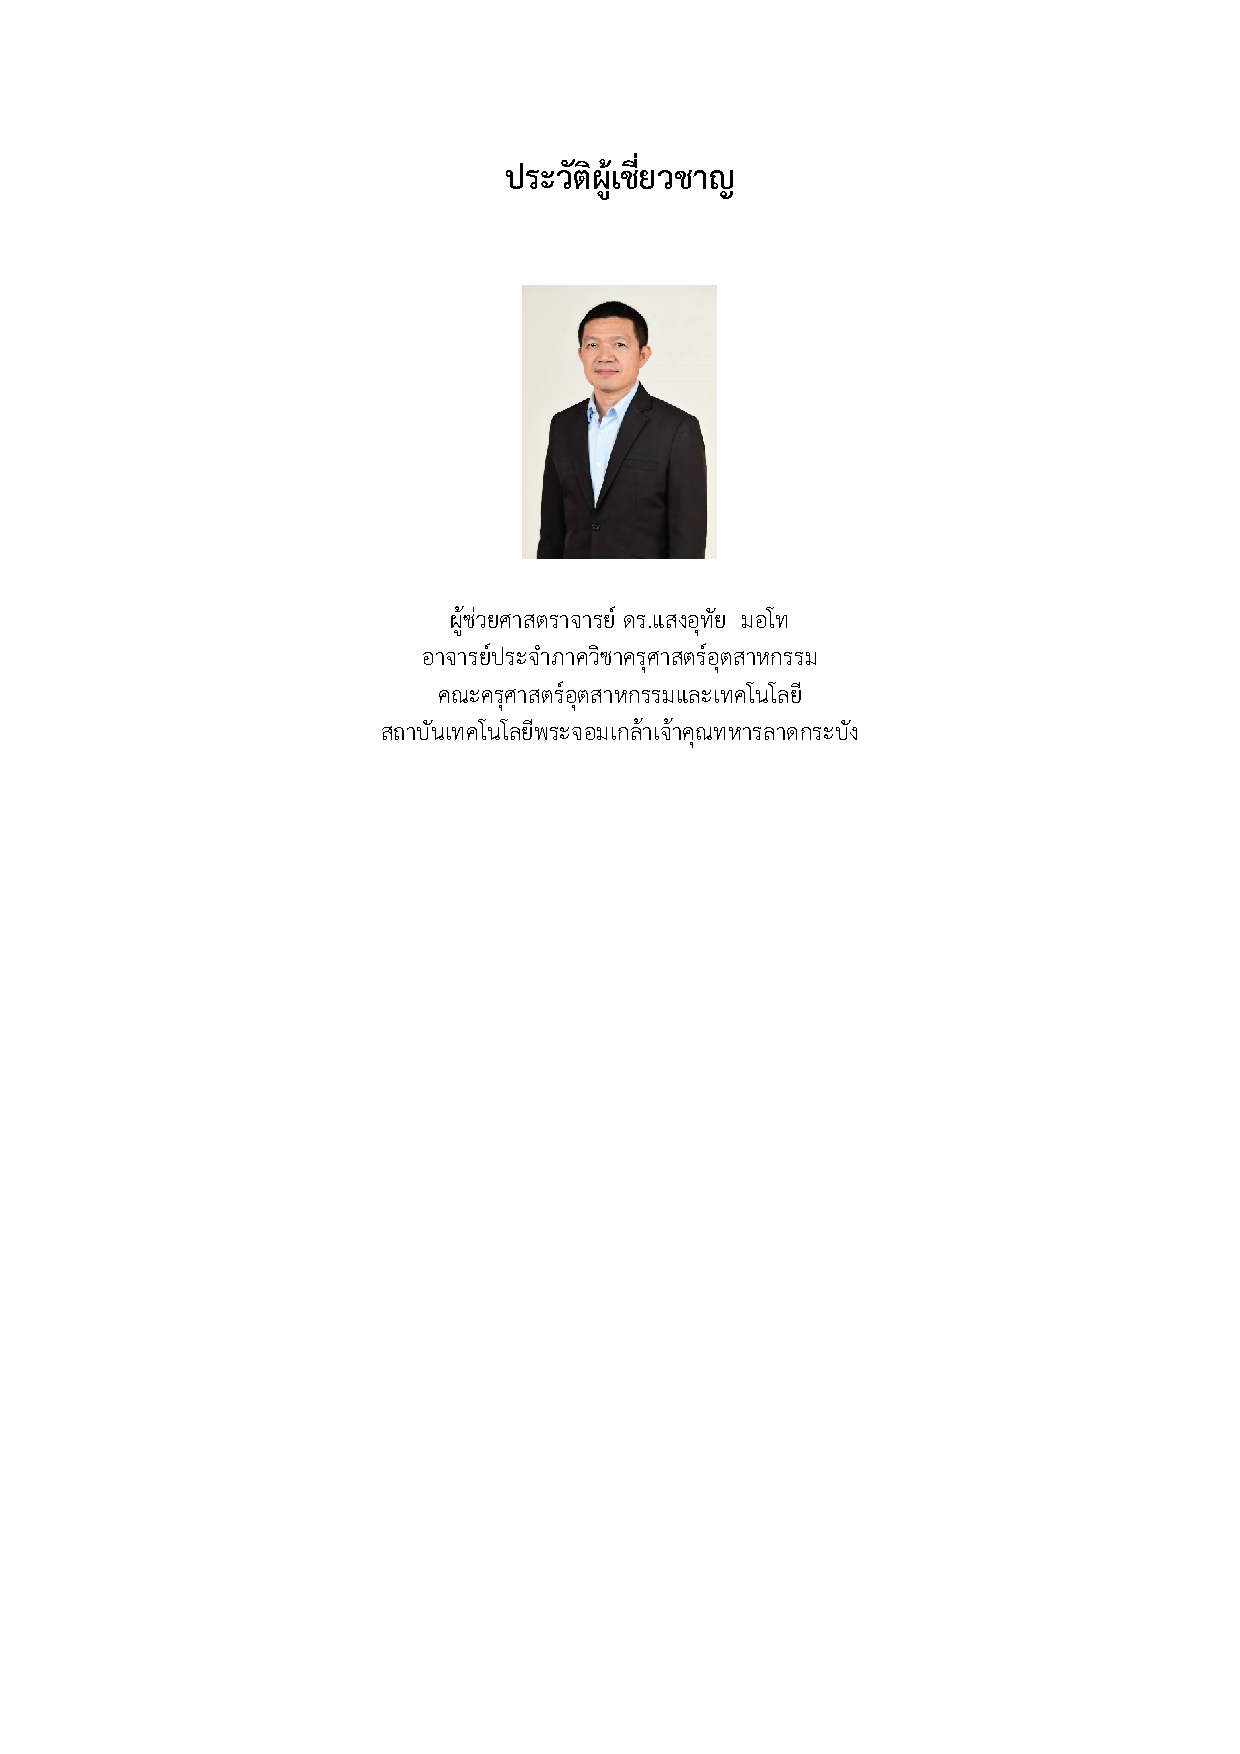
\includepdf[pages=1]{Word/ประวัติผู้เชี่ยวชาญ.pdf}
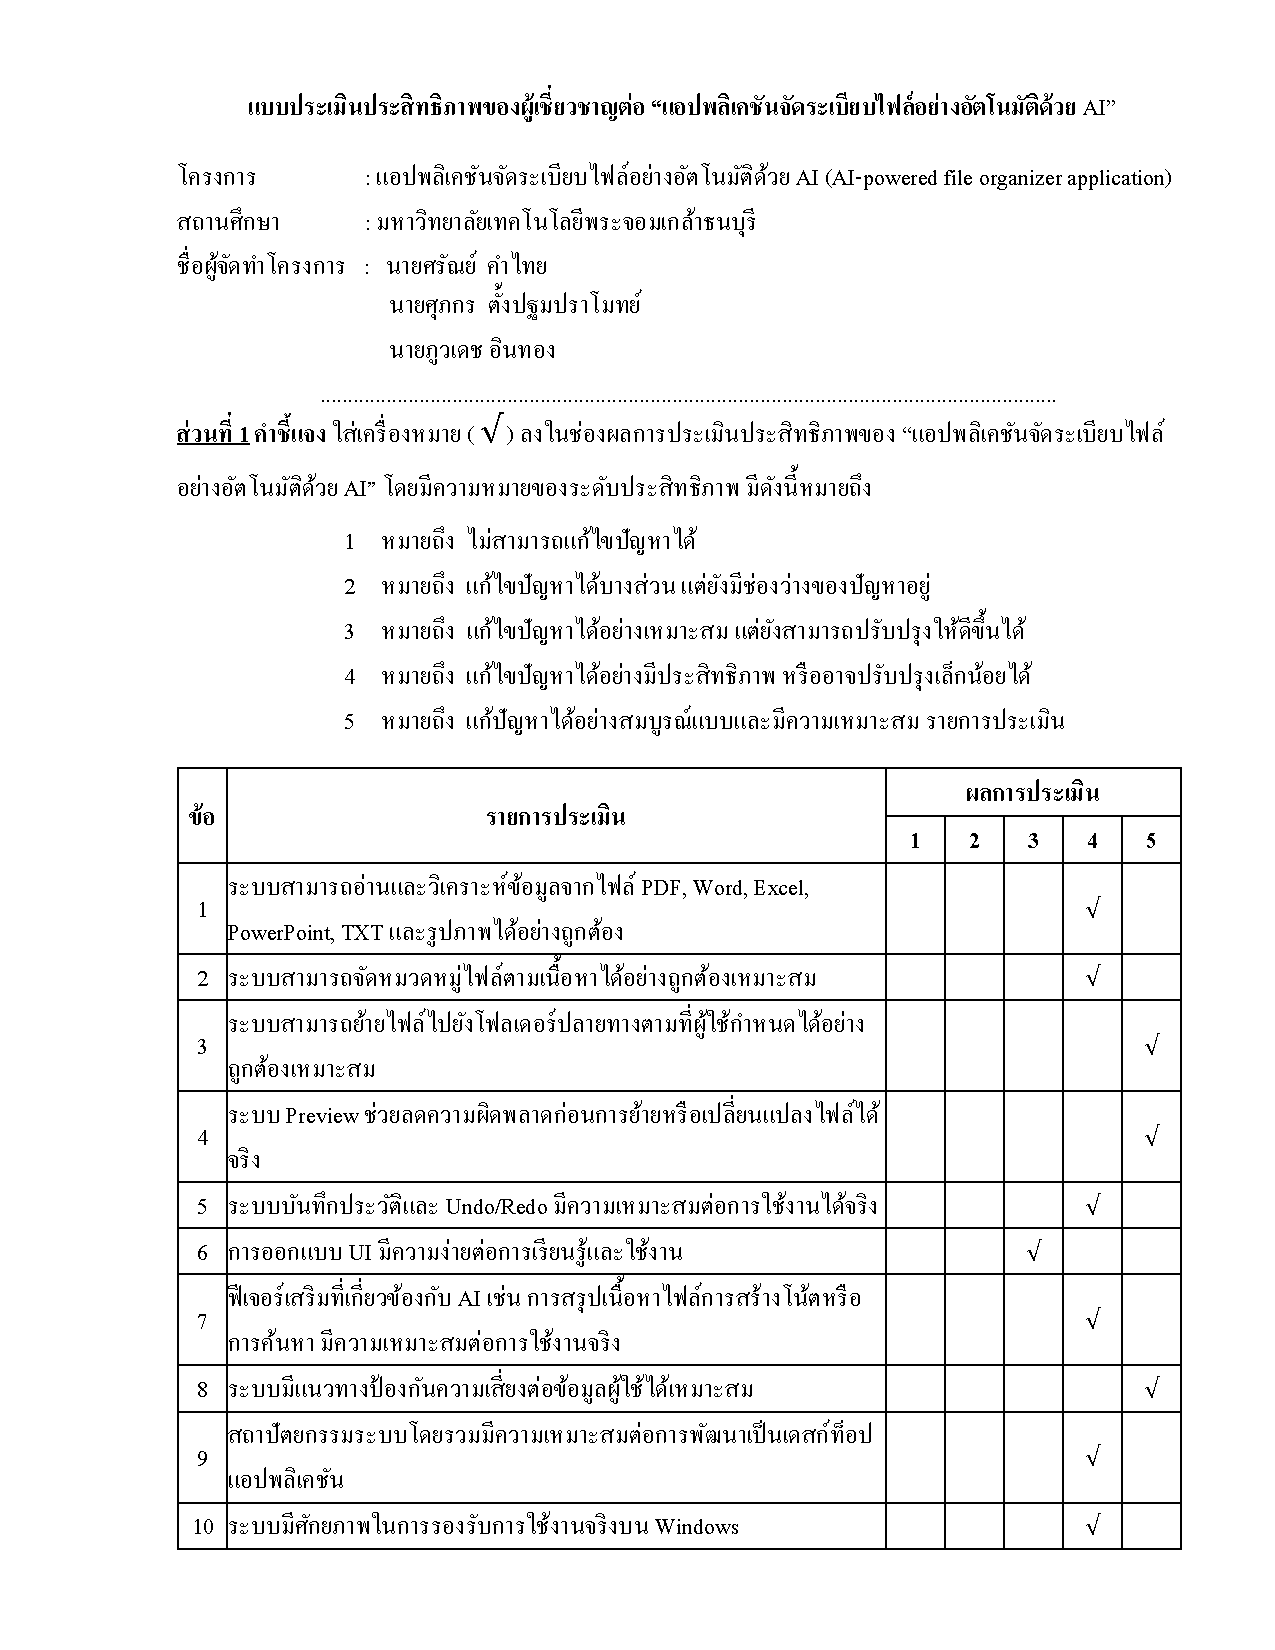
\includepdf[pages={1,2}]{Word/แบบประเมิณหาประสิทธิภาพของเครื่องมือ1.pdf}
% Expert 2: นายสนธยา เกื้อคีรี
\includepdf[pages=2]{Word/ประวัติผู้เชี่ยวชาญ.pdf}
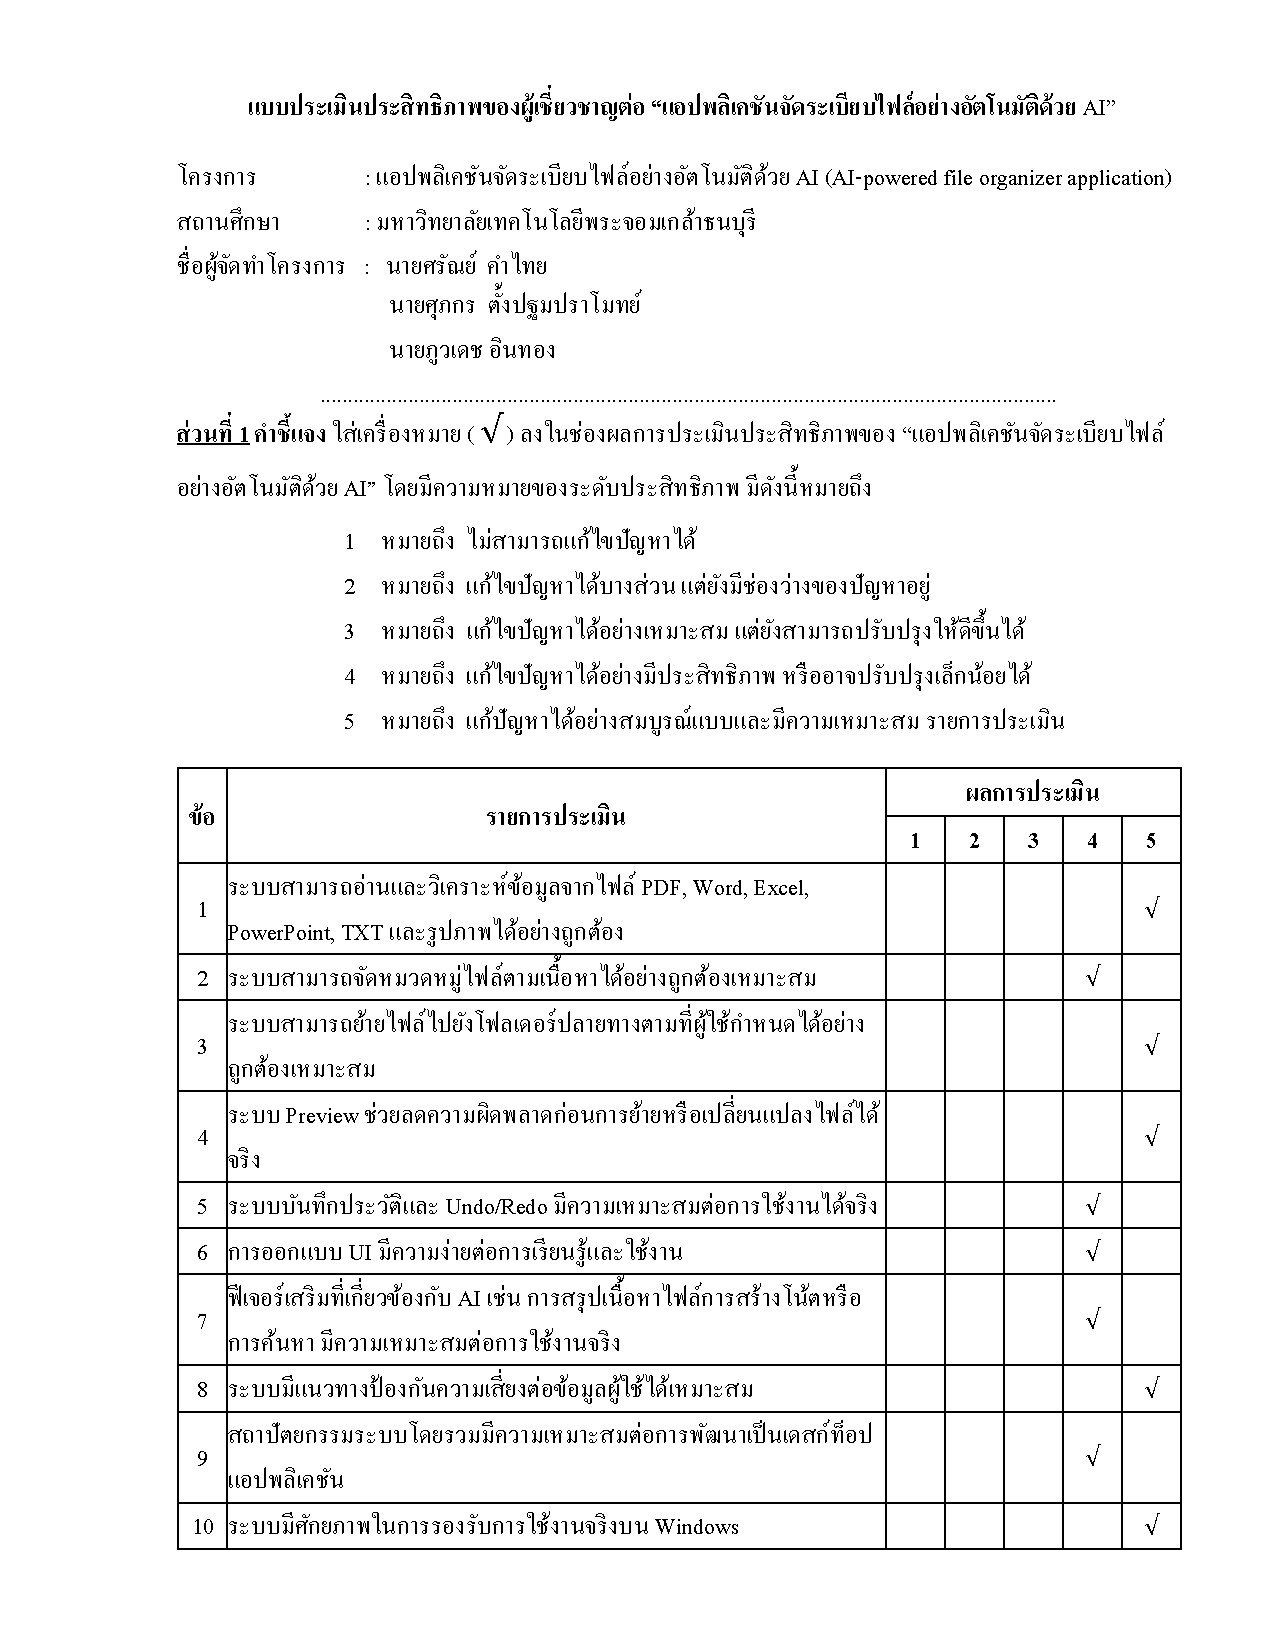
\includepdf[pages={1,2}]{Word/แบบประเมิณหาประสิทธิภาพของเครื่องมือ2.pdf}
% Expert 3: นายธีรวัฒน์ ณ นคร
\includepdf[pages=3]{Word/ประวัติผู้เชี่ยวชาญ.pdf}
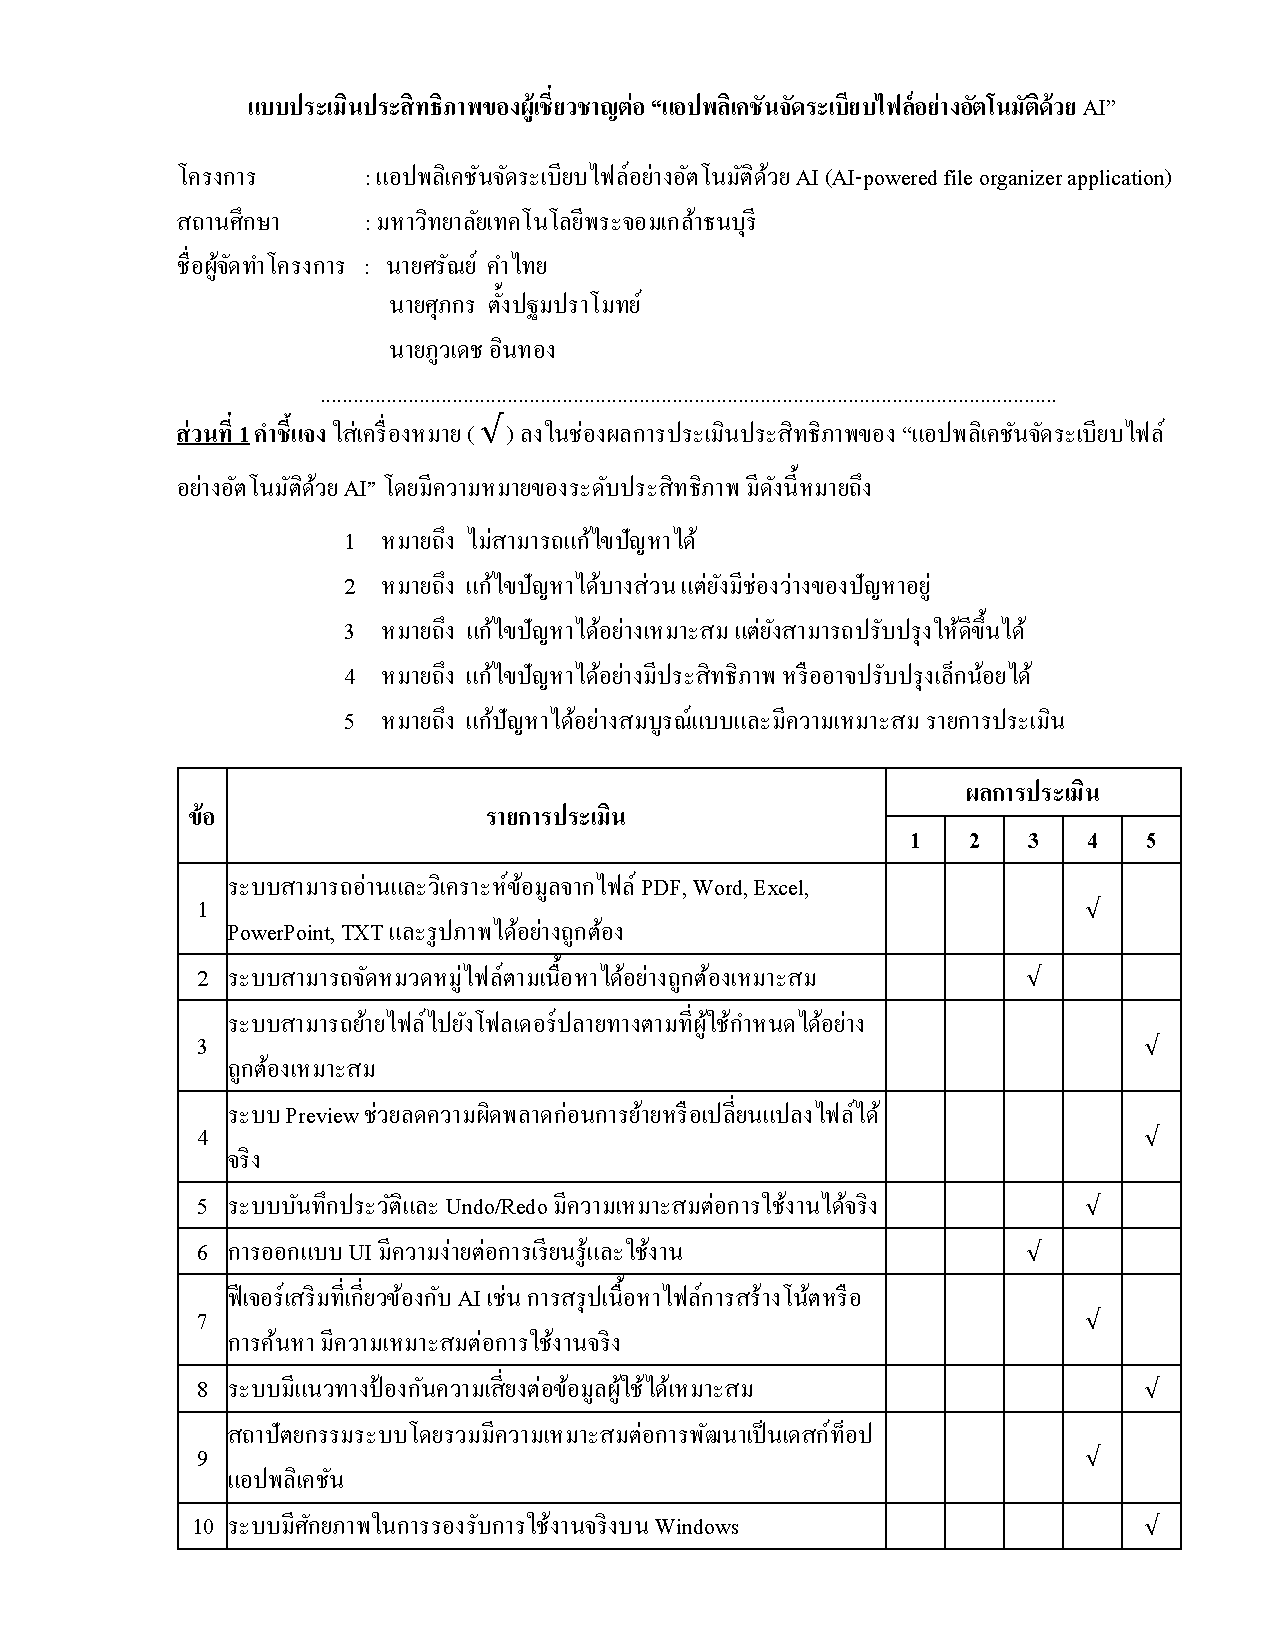
\includepdf[pages={1,2}]{Word/แบบประเมิณหาประสิทธิภาพของเครื่องมือ3.pdf}
\appendix{Installation Guide}

\section*{App Installation Guide}

This guide explains how to install KLIN using the Windows setup wizard.

\subsection*{1. Installation Overview}

The KLIN setup wizard guides you through five main stages: opening the installer, choosing the destination folder, confirming installation, waiting for the files to install, and finishing the setup. The screenshots in this document match the KLIN Windows installer shown during installation.

\subsection*{2. Requirements}

\begin{itemize}
\item A Windows computer that can run the KLIN application.
\item The KLIN installer file.
\item Administrator permission, if Windows requests it during installation.
\item Enough disk space in the selected destination folder.
\end{itemize}

\subsection*{3. Installation Steps}

\subsubsection*{3.1 Open the installer}

Run the KLIN setup file. The welcome screen appears. Click \textbf{Next} to continue or click \textbf{Cancel} if you want to exit the setup wizard.

\begin{figure}[H]
\centering
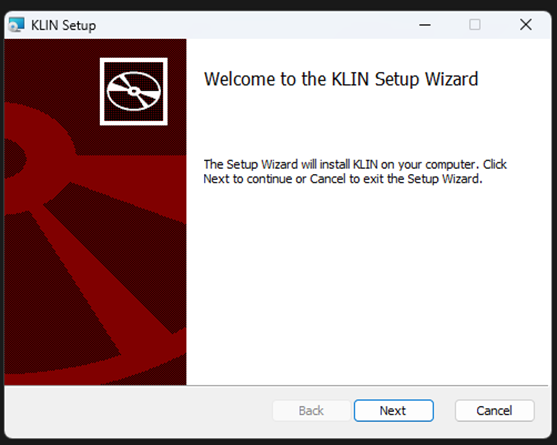
\includegraphics[width=0.75\textwidth]{figures/Picture4.png}
\caption{Step 1: Welcome to the setup wizard}
\end{figure}

\subsubsection*{3.2 Choose the installation folder}

The installer shows the default destination folder, usually \texttt{C:\textbackslash Program Files\textbackslash KLIN\textbackslash}. To use the default folder, click \textbf{Next}. To select a different location, click \textbf{Change} and choose another folder.

\begin{figure}[H]
\centering
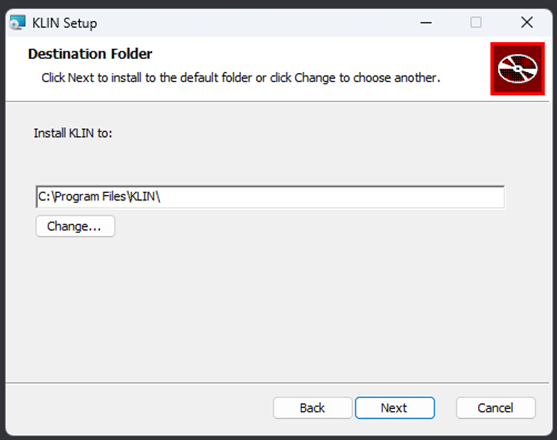
\includegraphics[width=0.75\textwidth]{figures/Picture5.png}
\caption{Step 2: Choose the destination folder}
\end{figure}

\subsubsection*{3.3 Confirm installation}

When the Ready to install KLIN screen appears, review the installation settings. Click \textbf{Install} to begin copying the application files to your computer.

\begin{figure}[H]
\centering
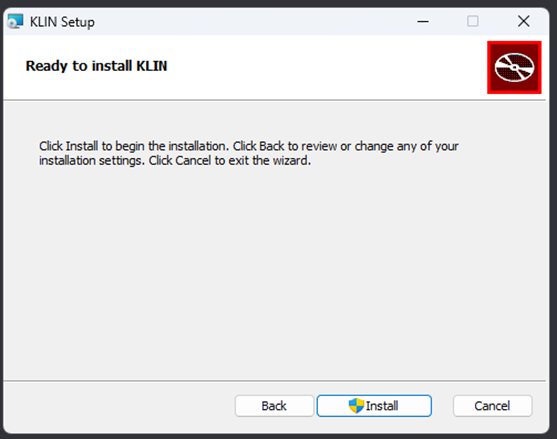
\includegraphics[width=0.75\textwidth]{figures/Picture6.png}
\caption{Step 3: Confirm that KLIN is ready to install}
\end{figure}

\subsubsection*{3.4 Wait for the installer}

The Installing KLIN screen shows the installation status. Wait until the process finishes. Do not close the setup wizard while installation is in progress.

\begin{figure}[H]
\centering
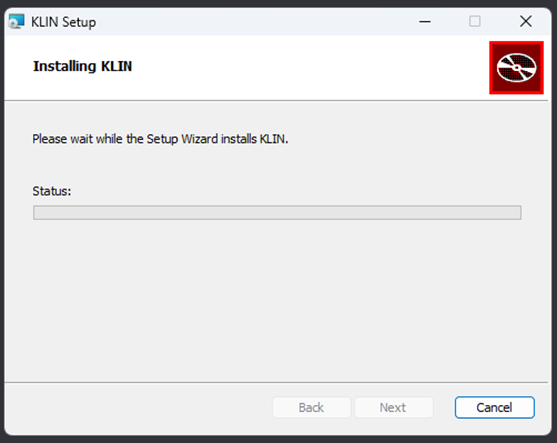
\includegraphics[width=0.75\textwidth]{figures/Picture7.png}
\caption{Step 4: Wait for installation to complete}
\end{figure}

\subsubsection*{3.5 Complete the setup}

When the Completed the KLIN Setup Wizard screen appears, the installation is finished. Keep \textbf{Launch KLIN} checked if you want to open the application immediately, then click \textbf{Finish}.

\begin{figure}[H]
\centering
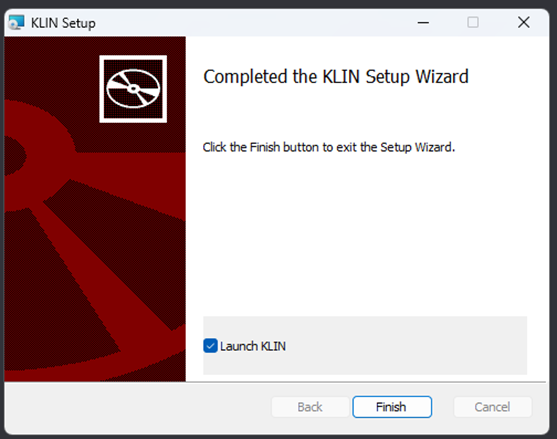
\includegraphics[width=0.75\textwidth]{figures/Picture8.png}
\caption{Step 5: Finish the installation}
\end{figure}

\subsection*{4. After Installation}

If \textbf{Launch KLIN} was selected, the application should open automatically after clicking \textbf{Finish}.
If it does not open automatically, search for KLIN from the Windows Start menu and launch it manually.
Check that the application opens correctly before deleting the installer file.

\subsection*{5. Troubleshooting}

\begin{longtable}{|p{0.35\textwidth}|p{0.55\textwidth}|}
\hline
\textbf{Issue} & \textbf{Suggested Solution} \\
\hline
The installer asks for permission & Click Yes if you trust the KLIN installer and want to continue. \\
\hline
Cannot install to Program Files & Run the installer as administrator or choose another folder using Change. \\
\hline
Installation seems stuck & Wait for a few minutes. If it does not continue, cancel the setup and run the installer again. \\
\hline
KLIN does not launch after Finish & Open KLIN from the Start menu, or restart Windows and try again. \\
\hline
\end{longtable}

\end{document}
